\documentclass[defaultstyle,11pt]{thesis}
\usepackage{paper,math}
\usepackage{hyperref}
\usepackage{natbib}
\usepackage{microtype}
\newcommand{\ATT}{\text{ATT}}
\newcommand{\dist}{\text{Dist}}

% ----
\newbool{INCLUDECOMMENTS}
\booltrue{INCLUDECOMMENTS}
\newcommand{\kyle}[1]{\textbf{Kyle: {#1}}}
% ----

\title{Three Essays on Applied Econometrics with Applications in Urban Economics}
\author{Kyle}{Butts}
\otherdegrees{
  B.S., University of California Santa Barbara, 2017 \\
  M.S., University of Colorado Boulder, 2020
}
\degree{Doctor of Philosophy}{Ph.D., Economics}
\dept{Department of}{Economics}

\advisor{Prof.}{Taylor Jaworski}
\reader{Adam McCloskey}
\readerThree{Brian Cadena}
\readerFour{Stephen Billings}
\readerFive{Richard Mansfield}

\abstract{  
  This dissertation contains three chapters that develop econometric tools for practical problems faced in the field of urban economics. 

  The first chapter `Dynamic Treatment Effect Estimation with Interactive Fixed Effects and Short Panels' studies inference on dynamic average treatment effect parameters for staggered interventions when parallel trends are only valid conditional on unobserved interactive fixed effects. Interactive fixed effects allow for the common setting where units are assigned to treatment based on their exposure to national macroeconomic shocks. Our identification strategy allows for any first stage set of moments that estimate the column space of the macroeconomic shocks including principal components, common correlated effects, quasi-differencing, and more. This allows us to estimate and control for the confounding common macroeconomics shocks. This result applies to data sets with either many or few pre-treatment time periods. We investigate the effect of Walmart openings on local economic conditions and demonstrate that our methods ameliorate pre-trend violations commonly found in the literature.

  The second chapter `Difference-in-Differences with Spatial Spillovers' addresses a common setting where treatment is assigned following geographic boundaries but the effects of the policies extend over space. Potential outcomes are modelled as a function of a unit's treatment status as well as their exposure to treatment status of other units. The paper highlights biases in standard estimators due to spillover effects. Then identification and estimation of treatment effects are discussed including in settings with staggered treatment adoption. The proposed methods are applied to reanalyze three empirical applications highlighting the impact of spillovers on policy evaluations.

  The final chapter `Difference-in-Differences with Geocoded Microdata' 
  formalizes a commonly-used estimator for the effects of spatially-targeted treatment with geocoded microdata. This estimator compares units immediately next to treatment to units slightly further away. I introduce intuitive identifying assumptions for the average treatment effect among affected units and illustrate problems when these assumptions fail. Since one of these assumptions requires knowledge of exactly how far treatment effects are experienced, I propose a new method that allows for nonparametric estimation following methods introduced in \citet{Cattaneo_Farrell_Feng_2019}. Since treatment effects can change with distance, the proposed estimator improves estimation by estimating a \emph{treatment effect curve}.
}
\dedication[Dedication]{	
  % NEVER use \OnePageChapter here.
	I dedicate this dissertation to my family: the queen Astrid, my boys Huckleberry and Archibald, and my best friend and teammate Hannah. You bring joy in my life every single day.
}
\acknowledgements{
  \OnePageChapter	% *MUST* BE ONLY ONE PAGE!
	
  I extend my heartfelt gratitude to my family for their unwavering love and support throughout my life. A special thank you to my mom for being my first phone call for every challenge and to Star for bringing brightness into my life.

  Thank you Rivka for helping me apply to programs and Phoenix for moving to Colorado and enjoying the mountains with me. I want to express my appreciation to all my classmates, including Brach, Jim, Alex, Payne, and Nick, for our first-year study sessions, research talk, and trips to the Downer. Thank you all for your valuable input and camaraderie. I am grateful to my coauthor Nicholas Brown for his collaboration and dedication.

  Thank you to my advisor, Taylor Jaworski, for allowing me to be creative and follow my interests; encouraging me to think broader and with more rigor; and for guiding me through challenges and supporting my growth every step of the way. Thank you to my committee and the fantastic economists I've met in graduate school for lending eyes on my work and giving encouragement.
}

% \ToCisShort	% use this only for 1-page Table of Contents
\LoFisShort	% use this only for 1-page Table of Figures
% \emptyLoF	% use this if there is no List of Figures
\LoTisShort	% use this only for 1-page Table of Tables
% \emptyLoT	% use this if there is no List of Tables

\begin{document}

\chapter{Dynamic Treatment Effect Estimation with Interactive Fixed Effects and Short Panels}
\vspace*{-15mm}
\begin{center}
  Authors: Kyle Butts and Nicholas Brown
\end{center}



% ------------------------------------------------------------------------------
\section{Introduction}
% ------------------------------------------------------------------------------

There are two common approaches for estimating the dynamic effects of a binary treatment in linear panel data models. Difference-in-differences estimators are one of the most popular causal inference tools and computationally simple but rely on strong parallel-trends assumptions. In many empirical settings, treatment is assigned non-randomly based on trends in economic variables, rendering this method unusable. For example, in urban economics, place-based policies target places with worsening labor markets \citep{neumark2015place}, new apartments are built in appreciating neighborhoods \citep{asquith2021local,pennington2021does}, and firms opening new stores in growing economies \citep{basker2005job,neumark2008effects}. Estimation of treatment effects in this setting is confounded by the pre-existing economic trends. It is common, though, that the causes of these trends are due to larger economic forces and not location-specific shocks. Continuing our examples, the national decline of manufacturing caused targeted manufacturing hubs to be declining, consumer trends for walkable neighborhoods cause certain neighborhoods to become increasingly demanded, and national changes to employment rates benefit certain counties. 

A recent growing literature models these kind of parallel trends deviations using an interactive fixed effects, but requires long panels for consistent estimation. While interactive fixed effects relax the parallel trends assumptions relied on by difference-in-differences, estimators requiring long panels are often impractical because of (i) lack of data for many years of outcomes, (ii) strong assumptions like serially uncorrelated outcomes, or (iii) the presence of structural breaks, e.g. recessions or structural changes to the macroeconomy, rendering previous time periods uninformative about the current economy. This paper proposes a treatment effect estimator under the more general interactive fixed effect model that is robust to certain violations of parallel trends while remaining consistent in short panels and under heterogeneous treatment effects. 

We model untreated potential outcomes, $y_{it}(\infty)$, as an interactive fixed effect model
\begin{equation}\label{eq:untreated_po}
    y_{it}(\infty) = \bm{f}_t' \bm{\gamma}_i + u_{it},
\end{equation}
where $\bm{F}_t$ is a $p \times 1$ vector of unobservable factors, $\bm \gamma_i$ is a $p \times 1$ vector of unobservable factor loadings, and $\expec{u_{it}} = 0$ for all $(i,t)$.\footnote{We follow \citet{Callaway_Santanna_2021} and define the state of not receiving treatment in the sample as `$\infty$'. This is useful in settings with staggered treatment timing where potential outcomes are denoted by the period where a unit start treatments.} We can view, as we did in the above examples, the factors $\bm{F}_t$ as macroeconomic shocks with factor loadings $\bm \gamma_i$ denoting a unit's exposure to the shocks. Another possibility lets the $\bm \gamma_i$ represent time-invariant characteristics with a marginal effect on the outcome $\bm{F}_t$ that changes over time.\footnote{\citet{Ahn_Lee_Schmidt_2013} suggest a wage equation where $\bm \gamma_i$ are unobserved worker characteristics of an individual and $\bm{F}_t$ are their time-varying prices or returns to those characteristics. See \citet{Bai_2009} for a collection of economic examples that justify the inclusion of a factor structure.} Note that this model nests the standard two-way error model when $\bm{F}_t' = (\lambda_t, 1)$ and $\bm \gamma_i' = (1, \mu_i)$; that is, $\bm{F}_t' \bm \gamma_i = \lambda_t + \mu_i$. The interactive structure allows for more general patterns of unobserved heterogeneity. Importantly, we allow for treatment to be correlated with a unit's exposure to macroeconomic shocks via their factor loadings $\bm{\gamma}_i$. 

For a concrete example, our empirical application focuses on estimating the effect of Walmart store openings on county-level employment. Estimation of a standard two-way fixed effect event-study model suggests that Walmart opened stores in counties that had higher retail employment growth prior to the opening (e.g. \citet{neumark2008effects}). In \autoref{fig:walmart_retail}, we present an event-study graph and overlay a line of best fit on the pre-treatment estimates. That the line is positive sloping and the estimates are different from zero at the 5\% level suggests that estimated positive impacts are due to pre-existing trends rather than the effect of Walmart per se. However, there seems to be a discrete jump when the Walmart opened. The goal then is to remove these pre-existing trends to isolate the treatment effect. It is plausible to assume that during their period of mass expansion, Walmart selected appealing locations based on their local demographic background and national economic trends, while ignoring transitory local economic shocks. Our framework allows this type of selection mechanism and effectively `controls' for these pre-existing trends in outcome.

Our main treatment effect identification result only requires fixed-$T$ consistent estimates of the column space of $\bm{F}_t$. Using the estimated factors, we compute a matrix that projects the pre-treatment outcomes onto the estimated post-treatment factors, imputing the untreated potential outcome for treated units. Averaging over the difference between the post-treatment observed outcomes and the estimated untreated potential outcomes gives a consistent estimator of average treatment effects. In specifications that include the two-way error model, we show how to explicitly remove the additive fixed effects with a double-demeaning transformation that maintains the common factor structure across treated groups and the never-treated group.

There are two major benefits of our general identification argument. First, fixed-$T$ consistent estimation of $\bm{F}_t$ is possible through a variety of approaches, which primarily includes quasi-differencing \citep{Ahn_Lee_Schmidt_2001,Ahn_Lee_Schmidt_2013,Callaway_Karami_2020} and cross-sectional averages \citep{Westerlund_Petrova_Norkute_2019,Juodis_Sarafidis_2022,Juodis_Sarafidis2021,Brown_Schmidt_Wooldridge2021} as a non-exhaustive list. These techniques allow the user to tailor their factor estimator to the specific data and problem under consideration, including how many pre-treatment time periods are available. Our identification result provides a recipe for using any consistent estimator of the factors to estimate treatment effects, opening up the large factor-model literature for causal inference methods. Second, our imputation method allows researchers to graph the estimated counterfactual untreated potential outcomes and the observed outcomes for treated units as a visual check for the parallel trends assumption, similar to a synthetic control plot.

We derive asymptotic properties of an imputation estimator with factor proxies that contain the true unobserved factors in their column space. The resulting estimator takes the form of a generalized method of moments (GMM) estimator, which allows estimation and inference via common statistical software. It is also consistent when the number of pre-treatment time periods is small.\footnote{Deriving the asymptotic distribution of treatment effects using large-$T$ factor estimators is left for future work.} One advantage of this estimator is that we can form statistical tests for the consistency of the two-way fixed effects (TWFE) estimator. These tests are practically useful since difference-in-differences is simple to implement. 

\subsection*{Relation to Literature}

Recent work has proposed `imputation' estimators for treatment effects using non-treated and pre-treatment observations to `impute' the untreated potential outcomes for the post-treatment observations \citep[e.g.][]{Borusyak_Jaravel_Spiess_2021,Gardner_2021,Wooldridge_2021}. However, these approaches only allow for level fixed effects and preclude interactions like in equation (\ref{eq:untreated_po}). \citet{Borusyak_Jaravel_Spiess_2021} allow a structure similar to equation \eqref{eq:untreated_po} but requires the the factors $\bm{F}_t$ be observed. We generalize these techniques by proposing an estimator that imputes the untreated potential outcomes under the more general (\ref{eq:untreated_po}) with unobserved interactive effects.

Current estimators that allow for selection based on a factor model either require (i) the number of time periods available is large, e.g. synthetic control \citep{abadie2021using}, factor-model imputation \citep{Xu_2017,Gobillon_Magnac_2016}, and the matrix completion method  \citep{Athey_et_al_2021,fernandez2021low}; or (ii) that an individual's error term $u_{it}$ is uncorrelated over time \citep{Imbens_Kallus_Mao_2021}.\footnote{\citet{Imbens_Kallus_Mao_2021} allow correlation within the post- and pre-treatment sets of the idiosyncratic errors, but assume independence between the two sets. This assumption is still strong in a static modeling context.} Both of these restrictions are non-realistic in many applied microeconomic data sets where the number of time periods is much smaller than the number of units and serial correlation of shocks is expected. Further, large-$T$ estimators often place restrictions on the dynamic heterogeneity of treatment. Our method requires neither large $T$ nor error term restrictions, but can still accommodate large-$T$ and unit-heterogeneous estimation strategies.

Our work contributes to an emerging literature on adjusting for parallel trends violations in short panels. \citet{freyaldenhoven2019pre} propose a similar instrumental variable type estimator in the presence of time-varying confounders. Their results rely importantly on homogeneous treatment effects. Their simulations show that heterogeneous treatment effects bias their estimates severely, while our estimator allows for arbitrary time heterogeneity. The most similar paper to our current approach is \citet{Callaway_Karami_2020}, who also allow for heterogeneous effects in short panels. They prove identification using a similar strategy to QLD and instrumental variables and derive asymptotic normality assuming the number of time periods is fixed. They require time-invariant instruments whose effects on the outcome are constant over time. Their instruments are valid for the QLD estimator in our application, but we also allow for time-varying covariates as instruments. They do not provide a general identification scheme like ours and so their results do not readily extend to other estimators like principal components or common correlated effects.

The rest of the paper is divided into the following sections: Section \ref{sec:theory} describes the theory behind our methods and presents identification results of the group-specific dynamic treatment effect parameters. Section \ref{sec:estimation} provides the main asymptotic theory for a particular QLD estimator. We also discuss practical concerns for practitioners. We include a small Monte Carlo experiment in Section \ref{sec:simulations} to examine the finite-sample performance of our estimator. Finally, Section \ref{sec:application} contains our application and Section \ref{sec:conclusion} leaves with some concluding remarks. 


% ------------------------------------------------------------------------------
\section{Model and Identification} \label{sec:theory}
% ------------------------------------------------------------------------------

We assume a panel data set with units $i = 1,\dots, N$ and periods $t = 1, \dots, T$. Treatment turns on in different periods for different units; we denote these groups by the period they start treatment. For each unit, we define $G_i$ to be unit $i$'s group with possible values $\{ g_1, \dots, g_G \} \equiv \mathcal{G} \subseteq \{ 2, \dots, T \}$. We follow \citet{Callaway_Santanna_2021} and denote $G_i = \infty$ for units that never receive treatment. We assume that $0 < P(G_i = g) < 1$ for all $g \in \mathcal{G} \cup \{ \infty \}$, so that the number of individuals in each group and the never-treated group grow with $N$. Treated potential outcomes are a function of group-timing, which we denote $y_{it}(g)$. For treatment indicators, we define the vector of treatment statuses $\bm d_{i} = (d_{i1},...,d_{iT})$ where $d_{it} = \mathbf{1}(t \geq G_i)$ and the indicator $D_{ig} = \mathbf{1}(G_i = g)$ if unit $i$ is a member of group $g$. Let $T_0 = \min_j \{ g_j \} - 1$ be the last period before the earliest treatment adoption. 

% We also introduce some matrix notation. For a vector $\bm x$ of length $T$, we use the subscript $\bm x_{t < g}$ to denote the first $g - 1$ elements and $\bm x_{t \geq g}$ to refer to the last $T - g + 1$ elements. This holds similarly for the rows of a matrix $\bm X$. 

Following \citet{Callaway_Santanna_2021}, we aim to estimate group-time average treatment effects on the treated:
\begin{equation}
  \ATT(g,t) = \tau_{gt} \equiv \expec{y_{it}(g)}{G_i = g} - \expec{y_{it}(\infty)}{G_i = g}
\end{equation}
These quantities represent the average effect of treatment at time $t$ for units that start treatment in period $g$ for $t \geq g$. It is trivial to estimate other averages as well in our framework, including averaging over all post-treatment observations to estimate an overall $\ATT$, and averaging over $(i,t)$ where $t - G_i = \ell$ to estimate event-study estimands $\ATT^\ell$'s. We discuss these and other extensions from \citet{Callaway_Santanna_2021} in Section \ref{sec:estimation}.

We now state our main identifying assumptions.
\begin{assumption}[\textbf{Sampling}]\label{asm:sampling}
The random vectors $\{ (\bm d_i, \bm \gamma_i, \bm u_i) \}$ are randomly sampled from an infinite population and has finite moments up to the fourth order. $\blacksquare$
\end{assumption}

\begin{assumption}[\textbf{Untreated potential outcomes}]\label{asm:untreated_po}
The untreated potential outcomes take the form
\begin{equation*}
  y_{it}(\infty) = \bm{F}_t' \bm \gamma_i + u_{it}
\end{equation*}
where $\expec{u_{it}}{\bm d_i, \bm \gamma_i} = 0$ for $t = 1,...,T$. $\blacksquare$
\end{assumption}

\begin{assumption}[\textbf{No anticipation}]\label{asm:no_anticipation}
For all units $i$ and groups $g \in \mathcal{G}$, $y_{it} = y_{it}(\infty)$ for $t < g$. $\blacksquare$ % Or, less strictly, we require $\expec{y_{it}}{G_i = g} = \expec{y_{it}(\infty)}{G_i = g}$ for $t < g$.
\end{assumption}

Assumption \ref{asm:untreated_po} imposes a factor-model for the untreated potential outcomes. The Online Appendix discusses the inclusion of covariates and the subsequent relaxation of assumption \ref{asm:untreated_po}. We allow for heterogeneous and dynamic treatment effects of any form, i.e. $y_{it}(g) = \tau_{igt} + y_{it}(\infty)$. We also allow arbitrary serial correlation among the idiosyncratic errors.\footnote{This condition may need to be strengthened for inference when $T \rightarrow \infty$.} We assume the common factors $\bm{F}_t$ are nonrandom parameters and the number of factors $p$ is fixed in the asymptotic analysis. 

Assumption \ref{asm:untreated_po} is more general than the standard difference-in-differences parallel trend assumption since we include the factor structure in our potential outcome model. In particular, it assumes that the error term is uncorrelated with treatment status \textit{after} controlling for the factor loadings. Treatment can still be correlated with contemporaneous shocks so long as the shocks, but not necessarily the exposure to them, are `common' across the sample. For example, our identification strategy is valid if workers select into a job training program based on their exposure (or adaptability) to macroeconomic productivity shocks. 

The two-way error model cannot generally accommodate differential exposure.\footnote{The following derivation is also shown in \citet{Callaway_Karami_2020}, but we are repeating it here for exposition.} In the more general factor model and \autoref{asm:untreated_po}, changes in untreated potential outcomes are given by
\begin{equation*}
  \expec{y_{it}(\infty) - y_{it-1}(\infty)}{G_i = g} = \lambda_t + (\bm{F}_t - \bm{F}_{t-1})' \expec{\bm \gamma_i}{G_i = g}
\end{equation*}
Unless either (i) the factor loadings have the same mean across treatment groups, $\expec{\bm \gamma_i}{G_i = g} = \expec{\bm \gamma_i}$, or (ii) the factors are time-invariant, then the standard parallel trends assumption that the group $g$ and the never-treated group follow common trends would not hold. If either of the two cases hold for all $g$ and $t$, the two-way error model is correctly specified.\footnote{We explicitly prove this result later.} However, these are knives edge cases which are not the focus of the paper. Our Assumption \ref{asm:untreated_po} allows for the factor loadings to be correlated with treatment timing and opens up treatment effect estimation for a much broader set of empirical questions.

The key econometric challenge lies in that we do not observe $y_{it}(\infty)$ whenever $d_{it} = 1$. Our goal is to consistently estimate $\expec{y_{it}(\infty)}{G_i = g}$ under equation (\ref{eq:untreated_po}) to consistently estimate group-time average treatment effects. \citet{Gardner_2021}, \citet{Wooldridge_2021}, and \citet{Borusyak_Jaravel_Spiess_2021} implicitly rely on this insight in studying the two-way error model. 

Prior attempts at estimating average treatment effects in a factor-model setting focus on finding conditions that allow for estimation of $\bm \gamma_i$ and $\bm{F}_t$ jointly as in \citet{Gobillon_Magnac_2016} and \citet{Xu_2017}, or a generalized version of a factor model as in \citet{arkhangelsky2021synthetic}. These techniques require the number of pre-treatment periods to grow to infinity and often place restrictions on both the dynamics of the treatment effects' distribution and the serial dependence among the idiosyncratic errors. Instead, we pursue identification noting that 
\begin{equation}\label{eq:untreated_cond_expectation}
\expec{y_{it}(\infty)}{G_i = g} = \bm{F}_t' \expec{\bm \gamma_i}{G_i = g}
\end{equation}
Therefore, we only need to estimate the \textit{average} of the factor loadings among a treatment group, which we can always do even with a small number of post-treatment time periods. We can then accommodate either a large or small number of pre-treatment periods and allow for estimation using a broad range of known strategies.

\subsection{\texorpdfstring{$\ATT(g,t)$}{ATT(g,t)} Identification}\label{sec:ATT_identification}

We begin by describing the intuition behind our identification result. Consider a unit subject to treatment at time $g$. Define $\bm y_{i,t<g}$ and $\bm y_{i,t\geq g}$ as respectively the first $(g-1)$ and last $(T-g+1)$ outcomes for unit $i$. Define $\bm{F}$ to be the matrix of factor shocks with rows given by $\bm{F}_t$. We similarly define $\bm{F}_{t < g}$ and $\bm{F}_{t \geq g}$ as the first and last rows of matrix $\bm{F}$. Equation \eqref{eq:untreated_cond_expectation} implies
\begin{equation}
  \expec{\bm y_{i,t < g}(\infty)}{ \bm G_i = g} = \bm{F}_{t < g} \expec{\bm \gamma_i}{\bm G_i = g}
\end{equation}
If the factors were observed, we could consistently estimate the mean values of the $p$-vector of average factor loadings for treated group $G_i = g$. More formally, if $\text{Rank}(\bm{F}_{t < g}) = p$, the coefficient from the population regression of $\expec{y_{i,t < g}(\infty) }{ G_i = g}$ on $\bm{F}_{t < g}$ is $\expec{\bm \gamma_i}{G_i = g}$. Equation \eqref{eq:untreated_cond_expectation} also gives us 
\begin{equation}
  \expec{\bm y_{i,t \geq g}(\infty)}{ \bm G_i = g} = \bm{F}_{t \geq g} \expec{\bm \gamma_i}{\bm G_i = g}
\end{equation}
for the post-treated outcomes. Assuming $\bm{F}$ is known (for now), we can predict $\expec{\bm y_{i,t}}{G_i = g}$ for $t \geq g$ by multiplying $\bm{F}_t$  by the OLS estimate from the prior regression. We then obtain $\expec{y_{it}(\infty)}{G_i = g}$ for the post-treatment outcomes, which we can subtract from $y_{i t}$ and average over the respective sample to obtain $\text{ATT}(g,t)$. 

We now define a useful matrix function for a more formal derivation of our main result. Given matrices $\bm X_1$ and $\bm X_0$ that are respectively $n \times k$ and $m \times k$, suppose $\text{Rank}( \bm X_0) = k$. We define the \textit{imputation matrix} 
\begin{equation}
  \bm P(\bm X_1, \bm X_0) \equiv \bm X_1 (\bm X_0' \bm X_0)^{-1} \bm X_0'
\end{equation}
This matrix takes a similar form to a projection matrix but ``imputes" the fitted values from regressing on $\bm X_0$ onto a different matrix $\bm X_1$. \citet{Gardner_2021} and \citet{Borusyak_Jaravel_Spiess_2021} implicitly uses the imputation matrix for an additive error model where $\bm X_1$ is the matrix of unit and time fixed effects and $\bm X_0$ is $\bm X_1$ with rows of zero whenever $d_{it} = 1$. When applying this matrix of factors to our outcomes, the post-treatment factors are multiplied by the factor loadings from the pre-treatment observations. In particular, we impute $y_{it}(\infty)$ by $\bm P(\bm{F}_{t}', \bm{F}_{t < g}) \bm y_{i,t < g}$ for $G_i = g$, similar to the bridge function identification scheme in \citet{Imbens_Kallus_Mao_2021}. However, because we only need a conditional mean assumption, we can allow arbitrary correlation between the idiosyncratic errors. 

The next theorem provides our main identification result:
\begin{theorem}\label{theorem:ATT_identification}
  Suppose $\bm{F}$ is known and $\text{Rank}(\bm{F}_{t \leq T_0}) = p$. Under Assumptions \ref{asm:sampling}, \ref{asm:untreated_po}, and \ref{asm:no_anticipation} for all $g \in \mathcal{G}$,
  \begin{equation}\label{eq:ATT_moments}
    \ATT(g,t) = \expec{y_{it} - \bm P(\bm{F}_{t}', \bm{F}_{t < g}) \bm y_{i,t < g}}{G_i = g}
  \end{equation}
  for $t \geq g$. 

  Moreover, let $\bm{F}^*$ be a full rank $T \times m$ matrix where $m < T_0$ and $\bm{F} \in \text{col}(\bm{F}^*)$, the column space of $\bm{F}^*$. Then the imputation matrix is invariant to $\bm{F}^*$
  \begin{equation}
    \bm P(\bm{F}_t^{*'}, \bm{F}^*_{t < g}) \bm{F}_{t < g} \bm \gamma_i = \bm{F}_t' \bm \gamma_i
  \end{equation}
  $\blacksquare$
\end{theorem}

All proofs are contained in the Online Appendix. Theorem \ref{theorem:ATT_identification} shows that we can identify the ATTs if we know the factor matrix. The second part of the theorem suggests that any rotation of the true factor matrix, $\bm{F}$, can be used in the imputation matrix. This is important because it is well understood that $\bm{F}_t$ and $\bm{\gamma}_i$ are not separately identified \citep{Ahn_Lee_Schmidt_2013,Xu_2017}. All of the estimators discussed so far can at best approximate the column space of the factors because both $\bm{F}_t$ and $\bm \gamma_i$ are unobserved. The second part of the theorem shows that our identification scheme allows for this class of estimators. 

\autoref{theorem:ATT_identification} shows we can apply these conclusions to any estimator that achieves fixed-$T$ consistency by asymptotically spanning the factor space. The most popular classes of these estimators examples include the common correlated effects \citep{pesaran2006estimation} and quasi-differencing \citep{Ahn_Lee_Schmidt_2013}. \citet{Westerlund_2020} shows that principal components can also fit in this class, so long as strong restrictions are met. As long as the column space of the factors are consistently estimated using the control sample, dynamic $\ATT$s are identified as in Theorem \ref{theorem:ATT_identification}, regardless of the normalization used for estimation. 

To present a general framework for the estimation of the factors, we formally present the identifying assumptions needed for factor space estimators:
\begin{assumption}\label{asm:factor_identification}
  There exists a $q \times 1$ vector of parameters $\bm{\theta}$ and a $T \times m$ function $\bm{F}(\bm{\theta})$ such that the following conditions hold:
  \begin{enumerate}[(i)]
    \item For some full-rank matrix $\bm{A}$, $\bm{F}(\bm{\theta}) \bm{A} = \bm{F}$ where $\text{Rank}(\bm{F}(\bm{\theta})) = m < T_0$ 
    \item There is a $s \times 1$ vector of moment functions $\bm g_{i\infty}(\bm{\theta})$ such that 
    \begin{equation}\label{eq:factor_moments}
      \expec{\bm g_{i\infty}(\bm{\theta})}{G_i = \infty} = \bm 0
    \end{equation}
    
    \item Let $\bm D_{\infty} = \expec{\nabla_{\bm{\theta}} \bm g_{i \infty}(\bm{\theta})}{G_i = \infty}$. Then $\text{Rank}(\bm D_{\infty}) = q$.
    \item $\expec{\bm g_{i \infty}(\bm{\theta}) \bm g_{i \infty}(\bm{\theta})'}{G_i = \infty}$ is positive definite. 
  \end{enumerate}
\end{assumption}
Part (i) implies that the estimated factors can be reduced to a finite dimension of estimable parameters. The matrix $\bm A$ is the full rank linear rotation that turns $\bm{F}(\bm{\theta})$ into $\bm{F}$. For the example estimators expressed above, $\bm{F}(\bm{\theta})$ asymptotically spans the unknown factors, $\bm{F}$. Parts (ii)-(iv) imply the parameters $\bm{\theta}$ are identified and consistently estimable. The parameters $\bm{\theta}$ themselves are often the result of an underlying normalization like in \citet{Ahn_Lee_Schmidt_2001,Ahn_Lee_Schmidt_2013}, \citet{Juodis_Sarafidis_2022,Juodis_Sarafidis2021}, and \citet{Callaway_Karami_2020}. Sometimes they are population moments estimated by cross-sectional averages like in \citet{Westerlund_Petrova_Norkute_2019} and \citet{Brown_Schmidt_Wooldridge2021}. 

% \citet{Chan_and_Kwok_2022} propose a principal components difference-in-differences estimator for unit-specific treatment effects, ruling out dynamic effects because of the large time series assumed in the asymptotic arguments. Our results show that estimation of the factors can be carried out using untreated observations and then applied to any post-treatment period for a time-specific ATT. This result relaxes their time-homogeneity assumption while also allowing for empirical examples where there are many time observations.
Assumption \ref{asm:factor_identification} is written with fixed-$T$ estimation and inference in mind. As mentioned before, accommodating general principal components estimation requires additional restrictions, as well as a large time series in the pre-treatment periods. However, the general identification result is the same and our estimator is still valid for estimating dynamic effects in the post-treatment period. \citet{Chan_and_Kwok_2022} study a principal components estimator for unit-specific treatment effects. Further research should formally derive the large-$T$ properties of our estimator using principal components in the first stage. 

\begin{remark}[Quasi-Long-Differencing]\label{remark:QLD}
A leading example of a set of moment equations for factor-space estimation is the quasi-long differencing (QLD) estimator of \citet{Ahn_Lee_Schmidt_2013}. They propose a QLD transformation given by 
\begin{equation}
  \bm H(\bm \theta) = (\bm I_{T-p}, \bm \Theta)
\end{equation}
where $\bm \Theta$ is a $(T-p) \times p$ matrix of unrestricted parameters and $\bm \theta = \text{vec}(\bm \theta)$\footnote{We reuse the ``$\bm \theta$" notation throughout the remainder of the text.}. They normalize the factors as 
\begin{equation}
  \bm{F}(\bm \theta) = 
  \begin{pmatrix}
    \bm \Theta\\
    -\bm I_p
  \end{pmatrix}
\end{equation}
so that $\bm H(\bm \theta) \bm{F} \bm \gamma_i = \bm 0$ by construction. We modify their proposed moment conditions to use just the never-treated group:
\begin{equation}
  \expec{g_{i\infty}(\bm{\theta})}{D_{i\infty} = 1} = \expec{\bm H(\bm \theta) \bm y_i \otimes \bm w_i}{D_{i\infty} = 1} = \bm 0
\end{equation}
where $\bm w_i$ is a vector of instruments that are exogenous with respect to the idiosyncratic error in \autoref{asm:untreated_po} but correlated with $\bm \gamma_i$. We discuss the choice of instruments $\bm w_i$ in more practical terms in \autoref{sec:application}.

While both approaches are valid in the first stage of our setting, we use the \citet{Ahn_Lee_Schmidt_2013} estimator because it is more general than \citet{Callaway_Karami_2020}. For one, they allow for a larger set of instruments. One identification strategy proposed by \citet{Callaway_Karami_2020} requires time-invariant covariates whose effects on $y_{it}$ are independent of time, meaning the researcher must decide which of the time-invariant observables have constant effects on the outcome. \citet{Ahn_Lee_Schmidt_2013} can allow for arbitrary time effects on covariates while still using those covariates as instruments. \citet{Ahn_Lee_Schmidt_2013} also give a road map to estimation based on weakly exogenous covariates that allows for dynamic modeling. This aspect of the estimator is left for future research.
$\blacksquare$
\end{remark}


\subsection{Two-Way Error Model}

We now demonstrate how to explicitly nest the standard two-way error model. While this structure is a special case of the factor model studied above, we consider the special case for two main reasons. First, eliminating the additive effects saves degrees of freedom to estimate the factor models; it may also provide efficiency by reducing the burden on first-stage factor estimators. Second, a thorough study of the additive model will provide insight into the link between TWFE estimation and more complicated and computationally involved factor model estimation. It will also allow us to show when TWFE estimation is consistent in the presence of interactive fixed effects. 

We first note that care must be taken when eliminating additive effects so that the overall factor structure is preserved. The methods in \citet{Borusyak_Jaravel_Spiess_2021}, \citet{Gardner_2021}, and \cite{Wooldridge_2021} that estimate the additive effects using the untreated sample will not maintain a common factor structure. For example, consider the first order conditions from the regression of $(1 - d_{it})y_{it}$ on unit and time effects. The estimators for the unit effect of a unit treated at time $g$ and a never-treated unit respectively satisfy
\begin{align}
  &\sum_{t = 1}^{g-1} (y_{it} - \widehat{\lambda}_t - \widehat{\mu}_i) = 0\\
  &\sum_{t = 1}^T (y_{it} - \widehat{\lambda}_t - \widehat{\mu}_i) = 0
\end{align}
The control sample will remove more time averages than in every treated sample, meaning the factors are demeaned using different subsamples. As such, the transformed factors are not equal across groups and so we cannot then use the control sample to estimate the factors for the treated samples. 

We first define the following averages for the purpose of removing the additive effects:
\begin{gather}
  \overline{y}_{\infty , t} = \frac{1}{N_{\infty}} \sum_{i = 1}^N D_{i \infty} y_{it} \\
  \overline{y}_{i,t\leq T_0} = \frac{1}{T_0} \sum_{t = 1}^{T_0} y_{it} \\
  \overline{y}_{\infty, t < T_0} = \frac{1}{N_{\infty} T_0} \sum_{i = 1}^N \sum_{t = 1}^{T_0} D_{i \infty} y_{it}
\end{gather}
where $\overline{y}_{\infty , t}$ is the cross-sectional averages of the never-treated units for period $t$, $\overline{y}_{i,t\leq T_0}$ is the time-averages of unit $i$ before any group is treated, and $\overline{y}_{\infty, t < T_0}$ is the total average of the never-treated units before any group is treated.

We then perform all estimation on the residuals $\tilde{y}_{it} \equiv y_{it} - \overline{y}_{\infty, t} - \overline{y}_{i,t < T_0} + \overline{y}_{\infty, t < T_0}$. These residuals are reminiscent of the usual TWFE residuals, except we carefully select this transformation to accomplish two things. First, this transformation leaves the treatment dummy variables unaffected to prevent problems with negative weighting when aggregating heterogeneous treatment effects \citep{Goodman-Bacon_2021,Borusyak_Jaravel_Spiess_2021}. Second, it preserves a common factor structure for all units and time periods\footnote{Such a transformation should not be used when considering the common correlated effects estimator because it would violate the CCE rank condition. See \citet{Brown_Butts_Westerlund_2023}.}. The TWFE imputation estimator of \citet{Gardner_2021}, \citet{Wooldridge_2021}, and \citet{Borusyak_Jaravel_Spiess_2021} would not share this property because they estimate $\mu_i$ and $\lambda_t$ based on the full sample $d_{it} = 0$, while we use a specific subsample.

This result is summarized in the following lemma:
\begin{lemma}\label{lemma:twfe_residuals}
  $\expec{\tilde{y}_{it}}{G_i = g} = \expec{d_{it}\tau_{it} + (\bm{F}_t - \overline{\bm{F}}_{t < T_0})' (\bm \gamma_i - \overline{\bm \gamma}_{\infty}) }{G_i = g}$ for $t = 1,...,T$ and $g \in \mathcal{G} \cup \{ \infty \}$ where $\overline{\bm{F}}_{t < T_0}$ is the average of $\bm{F}_t$ in the pre-treatment periods and $\overline{\bm\gamma}_\infty$ is the average of $\bm \gamma_i$ among the control units. $\blacksquare$
\end{lemma}

Lemma \ref{lemma:twfe_residuals} demonstrates how to explicitly nest the two-way error model model while allowing for a general common factor structure. Since we are not interested in inference on the factors themselves, this form will suffice for the imputation process. The transformed outcomes take the form
\begin{equation}
  \tilde{y}_{it} = d_{it} \tau_{it} + (\bm{F}_t - \overline{\bm{F}}_{t < T_0})' (\bm \gamma_i - \overline{\bm \gamma}_\infty) + \tilde{u}_{it}.
\end{equation}
For ease of exposition, we rewrite the above equation as:
\begin{equation}
  \tilde{y}_{it} = d_{it} \tau_{it} + \tilde{\bm{F}}_t' \tilde{\bm \gamma}_i + \tilde{u}_{it}.
\end{equation}

Lemma \ref{lemma:twfe_residuals} has the added benefit of showing us when the ATTs are identified by our TWFE transformation alone.
\begin{corollary}\label{cor:twfe_is_sufficient}
  Under Assumptions \ref{asm:sampling}-\ref{asm:no_anticipation}, $\ATT(g,t)$ is identified by the fixed effects imputation transformation if $\expec{\gamma_i}{G_i=g} = \expec{\gamma_i}$ for all $g \in \mathcal{G} \cup \{\infty\}$. $\blacksquare$
\end{corollary}
This result is an immediate consequence of Assumptions \ref{asm:sampling} -- \ref{asm:no_anticipation} as $\expec{\bm \gamma_j}{G_i = g} = \expec{\bm \gamma_i}$ for $j \neq i$ under random sampling. 
Corollary \ref{cor:twfe_is_sufficient} tells us that TWFE imputation is sufficient to estimate the ATTs, even when the factor structure exists, so long as the average factor loadings do not differ systemically with treatment status. Asymptotic normality of our imputation procedure under a two-way error model is studied in the Online Appendix. We also provide simple tests for mean independence of the factor loadings in Remark \ref{remark:twfe_testing}, i.e. consistency of the TWFE estimator. However, if the researcher believes a TWFE estimator is sufficient, they should use one of the other techniques mentioned above. Our method sacrifices potential efficiency by not using all observations to eliminate the additive effects in order to allow for additional interactive effects.



% ------------------------------------------------------------------------------
\section{Estimation and Inference}\label{sec:estimation}
% ------------------------------------------------------------------------------

This section considers estimation of the group-time average treatment effects. A major benefit of our approach is the simplicity of inference while allowing for a large number of possible estimation techniques in the first stage. Our moment conditions lead to a simple GMM estimator for which inference is standard and can be computed via routine packages in standard statistical software. Further, we can use the moment conditions to test the fundamental features of the model.

\subsection{Asymptotic Normality}

Equations \eqref{eq:ATT_moments} and \eqref{eq:factor_moments} provide us with the necessary moment conditions to estimate the ATTs. We collect them here in their unconditional form: 
\begin{gather*}
  \expec{\frac{D_{i\infty}}{\mathbb{P}(D_{i \infty} = 1)}\bm g_{i \infty}(\bm{\theta})} = \bm 0\\
  \expec{\bm g_{i g_G}(\bm{\theta}, \bm \tau_{g_G})} = \expec{ \frac{D_{ig_G}}{\mathbb{P}(D_{ig_G} = 1) } \left( \bm y_{i, t \geq g_G} - \bm P(\bm{F}_{t \geq g_G}(\bm{\theta}), \bm{F}_{t < g_G}(\bm{\theta})) \bm y_{i, t < g_G} - \bm \tau_{g_G} \right)} = \bm 0\\
  \vdots\\
  \expec{\bm g_{i 1}(\bm{\theta}, \bm \tau_{g_1})} = \expec{ \frac{D_{i g_1}}{\mathbb{P}(D_{i g_1} = 1) } \left( \bm y_{i, t \geq g_1} - \bm P(\bm{F}_{t \geq g_1}(\bm{\theta}), \bm{F}_{t < g_1}(\bm{\theta})) \bm y_{i, t < g_1} - \bm \tau_{g_1} \right)} = \bm 0
\end{gather*}
where $\bm \tau_g = (\tau_{gg},...,\tau_{gT})'$ is the vector of post-treatment treatment effects. We stack these over $g$ as $\bm \tau = (\bm \tau_{g_1}',...,\bm \tau_{g_G}')'$. The first set of moment conditions identify the factor space by Assumption \ref{asm:factor_identification} and the remaining moments identify the $\tau_{gt}$ via our imputation method.\footnote{We implicitly assume $\mathbb{P}(D_{ig_h} = 1)$ is strictly between $0$ and $1$ for every $g_h \in \mathcal{G} \cup \{\infty\}$.} Implementation requires replacing $\mathbb{P}(D_{ig} = 1)$ with its sample counterpart $N_g/N$. This setting can also accommodate cases as in \citet{Hahn_Liao_Geert_2018} where the factor structure is estimated nonparametrically in the first stage but the parametric estimator in the second stage is still $O_p(N^{-1/2})$. We leave this case for future study.


We need one final assumption to implement the asymptotically efficient GMM estimator:
\begin{assumption}\label{asm:variance_pd}
  $\expec{\bm g_{ig}(\bm{\theta}, \bm \tau_g) \bm g_{ig}(\bm{\theta}, \bm \tau_g)'}$ is positive definite for each $g \in \mathcal{G}$. $\blacksquare$
\end{assumption}

We collect the moment functions into the vector 
$$
\bm g_i(\bm{\theta}, \bm \tau) = (\bm g_{i\infty}(\bm{\theta})', \bm g_{ig_G}(\bm{\theta}, \bm \tau_{g_G})',...,\bm g_{ig_1}(\bm{\theta}, \bm \tau_{g_1})')'.
$$ 
In an abuse of notation, we assume $\bm g_{i\infty}$ is the moment function from equation \eqref{eq:factor_moments} but scaled by $D_{i\infty} / P(D_{i \infty} = 1)$. We define $\bm \Delta = \expec{\bm g_i(\bm{\theta}, \bm \tau) \bm g_i(\bm{\theta}, \bm \tau)'}$ which is positive definite by Assumptions \ref{asm:factor_identification} and \ref{asm:variance_pd}. Then our GMM estimator $(\widehat{ \bm{\theta}}', \widehat{ \bm \tau}')'$ solves
\begin{equation}\label{eq:minimization_problem}
  \min_{\bm{\theta}, \bm \tau} \left( \sum_{i = 1}^N \bm g_i(\bm{\theta}, \bm \tau) \right)' \widehat{\bm \Delta}^{-1} \left( \sum_{i = 1}^N \bm g_i(\bm{\theta}, \bm \tau) \right)
\end{equation}
where $\widehat{\bm \Delta} \plim \bm \Delta$ uses an initial consistent estimator of $(\bm{\theta}', \bm \tau')'$. 

\begin{theorem}\label{theorem:asymptotic_distribution}
  Under Assumptions \ref{asm:sampling}-\ref{asm:variance_pd}, $\sqrt{N}\big((\widehat{\bm{\theta}}', \widehat{\bm \tau}')' - (\bm{\theta}', \bm \tau')'\big)$ is jointly asymptotically normal as $N \rightarrow \infty$ and
  \begin{gather*}
    \sqrt{N}(\widehat{\bm{\theta}} - \bm{\theta}) \convd N \left( \bm 0, \left( \bm D'_{\infty} \bm \Delta_{\infty}^{-1} \bm D_{\infty} \right)^{-1} \right) \\
    \sqrt{N}(\widehat{\bm \tau}_{g_G} - \bm \tau_{g_G}) \convd N \left( \bm 0, \bm \Delta_{g_G} + \bm D_{g_G} \left( \bm D'_{\infty} \bm \Delta_{\infty}^{-1} \bm D_{\infty} \right)^{-1} \bm D_{g_G}'  \right)\\
    \vdots\\
    \sqrt{N}(\widehat{\bm \tau}_{g_1} - \bm \tau_{g_1}) \convd N \left( \bm 0, \bm \Delta_{g_1} + \bm D_{g_1} \left( \bm D'_{\infty} \bm \Delta_{\infty}^{-1} \bm D_{\infty} \right)^{-1} \bm D_{g_1}' \right)
  \end{gather*}
where $\bm D_g$ is the gradient of group $g$'s moment function with respect to $\bm{\theta}$ and $\bm \Delta_g$ is the variance of group $g$'s moment function. Further, the asymptotic covariance between $\sqrt{N}(\widehat{\bm \tau}_{g_h} - \bm \tau_{g_h})$ and $\sqrt{N}(\widehat{\bm \tau}_{g_k} - \bm \tau_{g_k})$ is given by $\bm D_{g_h} (\bm D_{\infty}' \bm \Delta_{\infty}^{-1} \bm D_{\infty})^{-1} \bm D_{g_k}'$. We derive the functional forms of the various matrices for the QLD estimator in the Appendix. $\blacksquare$
\end{theorem}

Valid inference is easy to obtain because we use a GMM framework. Analytic standard errors are computed and reported by most routine statistical packages implementing GMM estimation. We achieve the desired $\sqrt{N}$-convergence rate because we assume a $\sqrt{N}$-convergent estimator of the factor proxies. Examples include quasi-differencing, common correlated effects, and even principal components, though the latter also requires $T$ to go to infinity for the asymptotic results to hold\footnote{\citet{Ahn_Lee_Schmidt_2013} and \citet{Westerlund_Petrova_Norkute_2019} prove fixed-$T$, $\sqrt{N}$-asymptotic normality of the factor proxies for quasi-long-differencing and common correlated effects, respectively.}. Because we have proved asymptotic normality, one can also use the usual nonparametric panel bootstrap. We derive an asymptotically linear representation of the ATT estimates in the Appendix that also allow for the multiplier bootstrap as in \citet{Callaway_Karami_2020}. We also contain a discussion on deriving standard errors when the factors are not $\sqrt{N}$-convergent. 

The asymptotic distribution of $\sqrt{N}(\widehat{\bm \tau}_g - \bm \tau_{g})$ generally depends on the estimation of $\bm{\theta}$ in the first stage by the term $D_g (D_\infty' \Delta_\infty^{-1} D_\infty)^{-1} D_g'$. We can see directly from Theorem \ref{theorem:asymptotic_distribution} that a smaller $\text{Avar}(\sqrt{N}(\widehat{\bm{\theta}} - \bm{\theta}))$ leads to a smaller $\text{Avar}(\sqrt{N}(\widehat{\bm \tau}_g - \bm \tau_g))$ (in the matrix sense), strictly so when $\bm D_g$ has full rank. This result also suggests that more efficient estimation of the factors is an important avenue of future work and demonstrates why our general identification result is so powerful: we can use different estimators of the factors if we believe we can achieve substantial efficiency gains. 

Estimation of $\bm \tau_g$ is not dependent on the first stage estimation of $\bm{\theta}$ when $\bm D_g = \bm 0$. A sufficient condition for this equality occurs when the transformed factor loadings for group $g$ center about zero. The fixed-$T$ common correlated effects analysis of \citet{Westerlund_Petrova_Norkute_2019} implies such a condition. We may also think this condition holds in certain applications where the factor model is relevant. For example, suppose $\gamma_i$ is exposure to an information shock $f_t$ such that $\gamma_i \in [0,1]$ with probability one. If non-institutional investors of a given asset do not have access to privately held limited information, we would expect $\gamma_i \approx 0$ for units in said group. When the gradient $\bm D_g = \bm 0$ for a given $g$, the asymptotic variance of $\sqrt{N}(\widehat{\bm \tau}_g - \bm \tau_g)$ is just $\bm \Delta_g$. This quantity is simple to estimate via a nonparametric variance estimator. Let 
\begin{equation}\label{eq:nonparametric_variance}
  \widehat{\bm \Delta}_g = \frac{1}{N_g - 1} \sum_{i = 1}^N D_{ig} \left( \widehat{\bm \Delta}_{ig} - \widehat{\bm \tau}_{g_G} \right) \left( \widehat{\bm \Delta}_{ig} - \widehat{\bm \tau}_{g_G} \right)'
\end{equation}
where $\widehat{\bm \Delta}_{ig} = \bm y_{i, t \geq g} - \bm P(\bm{F}_{t \geq g}(\widehat{\bm{\theta}}), \bm{F}_{t < g}(\widehat{\bm{\theta}})) \bm y_{i, t < g}$. This estimator is sufficient to generate valid standard errors whenever $\bm D_g = \bm 0$.
\begin{theorem}\label{theorem:nonparametric_variance}
  Under Assumptions \ref{asm:sampling}-\ref{asm:variance_pd}, $\widehat{\bm \Delta}_g^{-1} \plim \bm \Delta_g^{-1}$.
\end{theorem}


\subsection{Extensions}

We conclude this section with a few extensions of our estimator to highlight the flexibility of our approach.

\begin{remark}[Limited Anticipation]
We can relax the limited anticipation assumption by simply redefining the last pre-treatment period as $q_g - 1$ and incorporate the additional $g - q_g$ periods into the moment conditions, so long as there are still enough pre-treatment periods to construct the imputation matrix. Then $\bm \tau_g$ is a $T - q_g + 1$ vector that makes treatment anticipation a testable hypothesis:
\begin{equation}
H_0: \tau_{g,q_g} = ... = \tau_{g,g-1} = 0 
\end{equation}
$\blacksquare$
\end{remark} 

\begin{remark}[Other Aggregate Treatment Effects]

Our estimation method can handle other aggregations of $y_{it} - \hat{y}_{it}(\infty)$. For example, one could aggregate over all post-treatment $(i,t)$ to estimate an overall $\ATT$ or over event-time indicators to estimate aggregate event-study estimates.\footnote{Alternatively, we allow for aggregation of $\ATT(g,t)$ estimates as in \citet{Callaway_Santanna_2021} by deriving the influence function in the Online Appendix.
} Researchers can perform heterogeneity analyses by aggregating for units with different values of $X_i$ like gender, race, or age to estimate a conditional $\ATT$. All one needs to do to estimate such aggregate effects is to correctly specify the unconditional treatment effect moment conditions. If there are \textit{a priori} restrictions on treatment effects as in \citet{Borusyak_Jaravel_Spiess_2021}, these can be imposed on the moment conditions as well. 

We can also derive pre-treatment ``placebo" effects by estimating a coefficient on the pre-treatment time periods. The imputation matrix that carries out this estimation is the usual projection matrix $\bm P(\bm{F}_{t \leq g}, \bm{F}_{t \leq g})$. Under the no anticipation assumption, 
\begin{equation}
  \expec{ \left( \bm I_{g} - \bm P(\bm{F}_{t \leq g}, \bm{F}_{t \leq g}) \right) \bm y_{i, t \leq g}}{G_i = g} = \bm 0
\end{equation}
so that the properly standardized vector of pre-treatment residuals is asymptotically normal. $\blacksquare$
\end{remark}


\begin{remark}[Plotting Estimates]\label{sec:plotting_estimates}

The proposed estimator can be used to produce estimates for $y_{it}(\infty)$ in all periods for the treated observations:
\begin{equation}
  \hat{y}_{it}(\infty) = \bm P(\bm{F}_t, \bm{F}_{t < g}) \bm y_{i, t<g} + \overline{y}_{\infty, t} + \overline{y}_{i, t<T_0} - \overline{y}_{\infty, t<T_0}
\end{equation}
where the first term on the right-hand side imputes $\hat{y}_{it}(\infty)$ and the last three terms in the sum `undo' the within-transformation\footnote{Leave this part out if you do not remove the additive effects by hand.}. In the pre-treatment periods, our estimates $\hat{y}_{it}(\infty)$ should be approximately equal to the observed $y_{it}$ under our assumptions. Similar to synthetic control estimators, comparing the imputed values to the true value can validate the `fit' of our model. However, since we have many treated units, doing so unit by unit is not practical. There are two complementary ways to aggregate treated units that will prove useful. 

First, one can aggregate over a group and plot the average of $y_{it}$ and the average of $\hat{y}_{it}(\infty)$ separately for each group $g \in \mathcal{G}$. This will create a set of `synthetic-control' like plots. To produce an `overall' plot, the observed outcome $y_{it}$ and the estimated untreated potential outcome $\hat{y}_{it}(\infty)$ should be `recentered' to event-time, i.e. reindex time to $e = t - G_i$, so that treatment is centered at event-time $0$. Then $y_{ie}$ and $\hat{y}_{ie}(\infty)$ can be aggregated for each value of event-time $e$. We produce such a plot in our empirical example.

\end{remark}

\begin{remark}[TWFE Specification Testing]\label{remark:twfe_testing}
  This paper is motivated by the fact that the two-way error model's generality is suspicious in practice. Therefore, we think a test of the two-way error structure versus a more complicated interactive effects model is of practical importance. \citet{Ahn_Lee_Schmidt_2013} discuss consistent estimation of $p$. Their tests have a new interpretation under this null hypothesis when testing for $p$ on the residuals $\tilde{y}_{it}$.

  \begin{theorem}
    If Assumption \ref{asm:sampling} and \ref{asm:untreated_po} hold with $\bm{F}_t' \bm \gamma_i = \bm 0$ almost surely, then $p = 0$. $\blacksquare$
  \end{theorem}
  If the null hypothesis is true, the more computationally burdensome QLD procedure is unnecessary for estimating the ATTs.\footnote{Even if TWFE is consistent, it is not necessarily more efficient than our procedure. See Section \ref{sec:simulations} for example.} Even if the two-way error model is unrepresentative of the factor structure, Corollary \ref{cor:twfe_is_sufficient} shows that mean independence of the factor loadings with respect to treatment timing is sufficient for consistency of TWFE. See the Online Appendix for an additional test of the equality of the factor loadings' conditional means. $\blacksquare$
\end{remark}


% ------------------------------------------------------------------------------
\section{Simulations}\label{sec:simulations}
% ------------------------------------------------------------------------------

We present a brief simulation study to compare our estimator to different TWFE specifications. We specifically study the quasi-differencing factor estimation approach of \citet{Ahn_Lee_Schmidt_2013} in the first stage because it is used in our empirical example. See \citet{Brown_Butts_Westerlund_2023} for simulation evidence for common correlated effects as the first stage estimator. We consider the setting where $T = 8$ and treatment turns on starting in period 6 implying $T_0 = 5$. We draw $N = 200$ observations, which is a relatively small number for a nonlinear estimation problem.

We generate untreated potential outcomes following equation (\ref{eq:untreated_po}). We consider the setting with one factor that we generate as a time-trend $f_t = t$.\footnote{In this particular case, if the researcher knew that $f_t$ took this form, then including unit-specific time-trends would fix this problem. However, we emphasize that $f_t$ is generally not observable. We include this simple form of $f_t$ so that the expected bias of TWFE is easy to compute: $t * (\expec{\gamma_i}{D_i = 1} - \expec{\gamma_i}{D_i = 0 })$.} We generate the time fixed effects as $\zeta_t = 0.75 * \zeta_{t-1} + \nu_{t}$ where $\nu_{t} \sim N(0,1)$. We generate the unit fixed effects as iid with $\mu_i \sim N(0, 4)$ and the factor loadings to be correlated with the unit fixed effects by drawing from $\gamma_i \sim N(\mu_i, 1)$. The error term is generated as an $AR(1)$ process with correlation coefficient $0.75$ and is uncorrelated with treatment status. We generate individual-level treatment effect heterogeneity by defining individual treatment effects $\tau_{i\ell}$ to be $\tau_\ell$ times the unit fixed effect but then re-scale the individual effects to have mean equal to $\tau_6 = 1$, $\tau_7 = 2$, and $\tau_8 = 3$ and for the variance of $\tau_{i\ell}$ to be one. For example, $\tau_{i6} = (\mu_i + 2)/2$. 

We generate a covariate $w_i = \gamma_i + \xi_i$ where $\xi_i$ is white-noise measurement error. $w_i$ will be used as a covariate in some TWFE specifications and as our instrument for our factor-model estimation. In the baseline simulation, we consider the case where $\xi_i \sim N(0, 1)$, which creates a signal-to-noise ratio for the instrument of $1/2$. In a set of simulations, we vary the level of noise to see how the instrument strength affects estimates. These results will allow us to compare our methods to those that use noisy measurements of unobserved heterogeneity.

We consider three data-generating processes. First, we consider the true two-way error model where there are no interactive effects. In this case, the two-way fixed effects estimator should be unbiased. Second, we generate outcomes with the factor model described above. Treatment is then assigned completely randomly with probability of treatment at 50\% for all units. This implies that the factor loadings are uncorrelated with treatment status, which Corollary \ref{cor:twfe_is_sufficient} shows is sufficient for the TWFE imputation procedure to be consistent. Third, we generate treatment with probability increasing in the factor loading such that parallel trends fail (since treated units are more exposed to the time-trend in $f_t$). In particular, we form the term
\begin{equation}
\pi_i = 0.5 + \frac{\gamma_{i}}{\max_i \gamma_i - \min_i \gamma_i}
\end{equation}
We normalize this term by the mean of $\pi_i$ so that the unconditional probability of treatment stays at 50\%.

We estimate event-study treatment effects using four estimators. First, we estimate the classical two-way error model using ordinary least squares (OLS), i.e. the TWFE estimator. Second, we estimate the two-way error model using the imputation estimator proposed by \citet{Borusyak_Jaravel_Spiess_2021} and \citet{Gardner_2021}.\footnote{We use the R package \texttt{did2s} \citep{butts2022did2s} for estimation.} Third, we augment the two-way error model by including a noisy measure of the factor loadings. This is sometimes done by applied researchers in an attempt to control for confounders. That is, they model outcomes as 
\begin{equation}\label{eq:twfe_w_cov}
  y_{it} = \mu_i + \lambda_t + w_i \beta_t + u_{it}
\end{equation}
where $w_i$ is a time-invariant covariate and $\beta_t$ allows for trends to vary based on $w_i$. In the case where $w_i = \gamma_i$, i.e. the factors are observable, this model is correctly specified. However, when $\text{Var}(\xi_i) > 0$, i.e. the covariates are noisy measures for the underlying factor loadings, model (\ref{eq:twfe_w_cov}) will only partially absorb the factor model. We compare this method to our estimator using the QLD transformation of \citet{Ahn_Lee_Schmidt_2013} to estimate the factors.\footnote{We use the \texttt{Optim.jl} package for GMM estimation \citep{mogensen2018optim}.} The covariate $w_i$ is our instrument in the first stage to estimate the QLD parameters. See Remark \ref{remark:QLD}.

\begin{table}
\def\arraystretch{1.25}
\caption{Monte Carlo Simulation}
\label{tab:monte_results_pt}

\begin{adjustbox}{width=\textwidth}
\begin{tabular}{@{} >{\raggedright}p{3.2cm} @{\extracolsep{4pt}}cccccc @{}} 
  % Head
  \toprule \addlinespace[3mm]
  
  \multicolumn{7}{@{}l}{
    \textbf{Panel A:} Two-way error model.
  } \\
  \midrule \addlinespace[3mm]
  
  & $\text{Bias}\ \big(\hat{\tau}_6 \big)$ & $\text{MSE}\ \big(\hat{\tau}_6\big)$
  & $\text{Bias}\ \big(\hat{\tau}_7 \big)$ & $\text{MSE}\ \big(\hat{\tau}_7\big)$
  & $\text{Bias}\ \big(\hat{\tau}_8 \big)$ & $\text{MSE}\ \big(\hat{\tau}_8\big)$ 
  \\
  \cmidrule{2-7}
  
  TWFE & 0.00 & 0.01 & -0.00 & 0.02 & 0.00 & 0.02 \\ 
  TWFE Imputation & 0.01 & 0.01 & 0.00 & 0.02 & 0.01 & 0.02 \\ 
  TWFE Imputation with Covariates & 0.01 & 0.01 & 0.00 & 0.02 & 0.01 & 0.02 \\ 
  Factor Imputation & -0.00 & 0.04 & -0.01 & 0.11 & -0.01 & 0.24 \\ 


  \midrule \addlinespace[3mm]
  \multicolumn{7}{@{}l}{
    \textbf{Panel B:} Factor Model. Parallel Trends Hold
  } \\
  \midrule \addlinespace[3mm]
  
  & $\text{Bias}\ \big(\hat{\tau}_6 \big)$ & $\text{MSE}\ \big(\hat{\tau}_6\big)$
  & $\text{Bias}\ \big(\hat{\tau}_7 \big)$ & $\text{MSE}\ \big(\hat{\tau}_7\big)$ 
  & $\text{Bias}\ \big(\hat{\tau}_8 \big)$ & $\text{MSE}\ \big(\hat{\tau}_8\big)$ 
  \\
  \cmidrule{2-7}
  
  TWFE & 0.00 & 0.11 & 0.00 & 0.43 & 0.01 & 0.95 \\ 
  TWFE Imputation & 0.00 & 0.94 & 0.00 & 1.67 & 0.01 & 2.60 \\ 
  TWFE Imputation with Covariates & 0.00 & 0.17 & 0.00 & 0.29 & 0.01 & 0.44 \\ 
  Factor Imputation & -0.00 & 0.02 & -0.00 & 0.03 & 0.00 & 0.05 \\ 

  \midrule \addlinespace[3mm]
  \multicolumn{7}{@{}l}{
    \textbf{Panel C:} Factor Model. Parallel Trends Do Not Hold
  } \\
  \midrule \addlinespace[3mm]
  
  & $\text{Bias}\ \big(\hat{\tau}_6 \big)$ & $\text{MSE}\ \big(\hat{\tau}_6\big)$
  & $\text{Bias}\ \big(\hat{\tau}_7 \big)$ & $\text{MSE}\ \big(\hat{\tau}_7\big)$ 
  & $\text{Bias}\ \big(\hat{\tau}_8 \big)$ & $\text{MSE}\ \big(\hat{\tau}_8\big)$ 
  \\
  \cmidrule{2-7}
  
  TWFE & -1.63 & 2.77 & -3.27 & 11.05 & -4.90 & 24.84 \\ 
  TWFE Imputation & -4.90 & 24.81 & -6.53 & 44.12 & -8.16 & 68.93 \\ 
  TWFE Imputation with Covariates & -0.92 & 1.06 & -1.22 & 1.88 & -1.53 & 2.93 \\ 
  Factor Imputation & 0.01 & 0.03 & 0.01 & 0.05 & 0.02 & 0.09 \\ 
  
  
  \bottomrule
\end{tabular}
\end{adjustbox}

\note{This table presents a set of simulations with 10000 simulations. Each panel contains one of three data-generating processes described in the text. Each row in a panel consists of one of the four treatment effect estimators as described in the text. The columns report average bias and  mean-squared error for the three post-treatment treatment effects.}

\end{table}

Results are presented in table \ref{tab:monte_results_pt}. Each panel presents results from each of the three data-generating processes described above. For each estimate, we present the average bias for the estimate as well as the mean-squared error. For Panel A where the outcomes are generated under the two-way fixed effect model (i.e. without a factor structure), all estimators are unbiased for the treatment effects, but the more robust factor imputation pays an efficiency cost with larger mean-squared error. However, this flips in Panel B where outcomes are generated under a factor model but with parallel trends holding for the two-way error model. In this case, all estimators are still unbiased but the factor imputation estimator is the most efficient because it absorbs the factor-structure that is present in the error term for the two-way error model.

Turning to where parallel trends does not hold in Panel C, we see that only our factor-imputation estimator is unbiased. This result emphasizes that our estimator is robust for parallel trend violations coming from differential exposure to macroeconomic factors. The magnitude of bias present in the two-way error models is growing from $\tau_6$ to $\tau_8$ due to the factor being a linear time-trend, implying parallel trend deviations grow worse over time. 

It is worth noting that while including $w_i \beta_t$ in the model does remove some bias, the estimates still perform worse than our imputation procedure due to $w_i$ being a noisy measure. To highlight the problems with noisy proxies for factor loadings, figure \ref{fig:noisy_w} presents a set of simulation results where the covariate $w_i$ has different amount of noise added in. In particular, we choose different values of $\text{Var}(\xi_i)$ to have different signal-to-noise measures. The signal-to-noise definition is 
\begin{equation}
    \text{signal to noise ratio} = \frac{\text{Var}(\gamma_i)}{\text{Var}(\gamma_i) + \text{Var}(\xi_i)}
\end{equation}
For each signal to noise ratio, we estimate the TWFE imputation estimator with covariates and the factor model imputation estimator. Figure \ref{fig:noisy_w} presents the results of estimates for $\tau_8$. At one extreme, where the signal to noise ratio is approximately 0, i.e. $\xi_i$ is white noise, the estimated bias for the TWFE imputation estimator is the same as the TWFE imputation estimator that does not include covariates. At the other extreme, where the signal to noise ratio is approximately 1, i.e. $w_i = \gamma_i$, the bias is completely removed. Regardless, the factor model imputation estimator is unbiased in all cases. This experiment echos the results of \citet{kejriwal2021efficacy}. However, we note that our results are still generous to estimators that use such noisy measure because we generate $w_i$ as an unbiased estimator of $\gamma_i$. The instrument requirement for QLD estimation does not require unbiased estimation of $\bm \gamma_i$ for identification of the normalized parameters.

\begin{figure}
\begin{adjustbox}{width=.8\textwidth, center}
  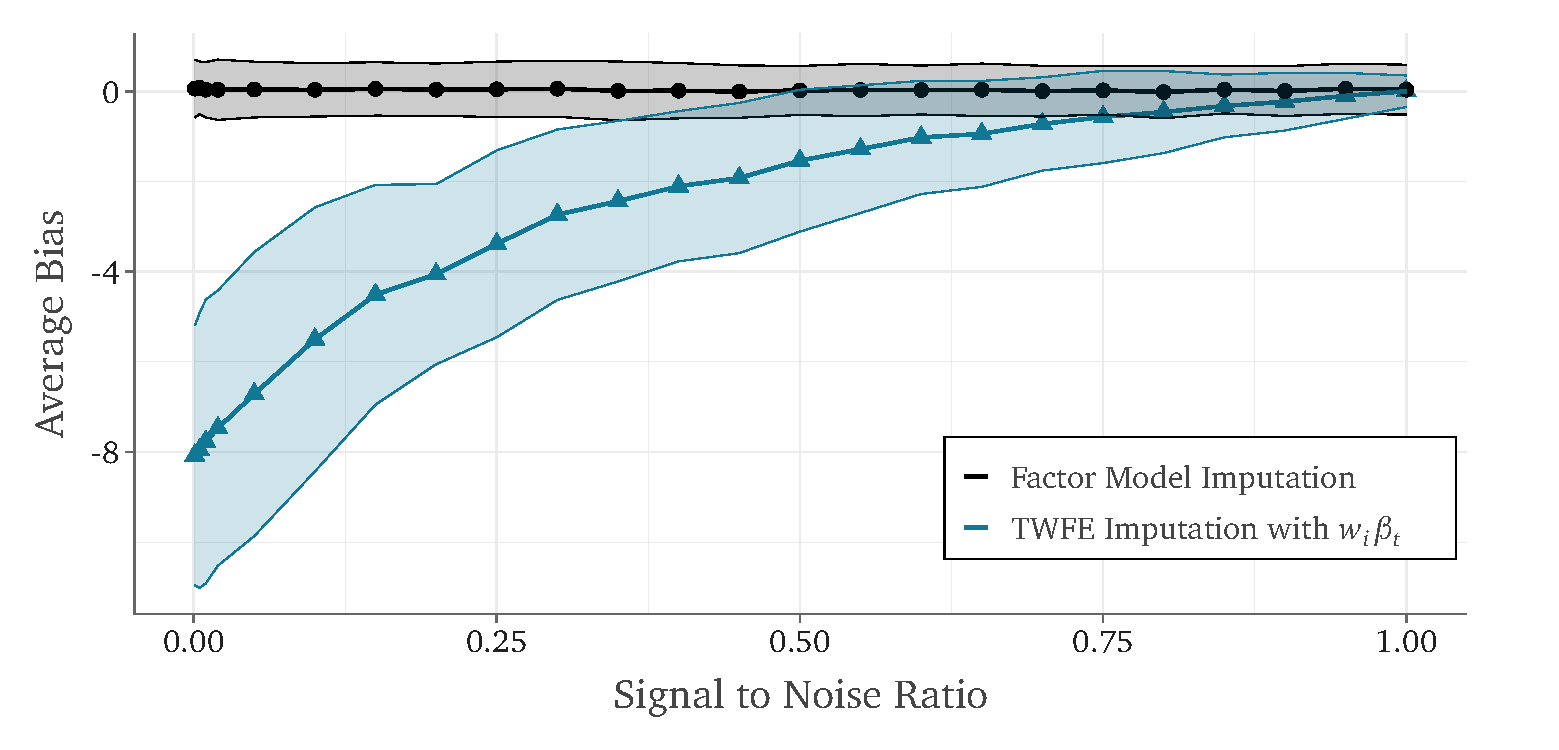
\includegraphics{figures/generalized/simulation-bias_signal_to_noise.pdf}
\end{adjustbox}
\caption{Bias of TWFE Imputation with Covariates}\label{fig:noisy_w}
\note{This figure plots the average and empirical 95\% confidence intervals for treatment effect estimates in the final period, $\hat{\tau}_8$. We estimate the TWFE imputation estimator that includes $w_i \beta_t$ linearly in the model and our the factor imputation we propose using $w_i$ instead as an instrument. We vary the signal to noise ratios of $w_i$ to make it a better or worse measure for the factor loading. For each signal to noise ratio, we run 5000 simulations.}

\end{figure}


% ------------------------------------------------------------------------------
\section{Application}\label{sec:application}
% ------------------------------------------------------------------------------

We revisit the literature on estimating local labor market effects of Walmart store openings \citep{basker2005job, neumark2008effects, volpe2022economic}. The primary identification concern is that Walmart targets where to open stores based on local economic trajectories \citep{neumark2008effects}. For instance, if Walmart targeted areas with positive underlying economic fundamentals in anticipation of their growing consumptive expenditures, then the non-treated counties would fail to be a valid counterfactual group in the two-way error model. Indeed, we observe significant differences in both employment trends for treated counties in our data. \citet{volpe2022economic} point to conflicting results on retail employment with two leading papers finding effects of opposite signs. Employing different instrumental variable strategies, \citet{basker2005job} finds positive effects on retail employment while \citet{neumark2008effects} finds negative effects. For this reason, we revisit this question with an alternative strategy to answer this question. 

We construct a dataset following the description in \citet{basker2005job}. In particular, we use the County Business Patterns dataset from 1964 and 1977-1999, subsetting to counties that (i) had more than 1500 employees overall in 1964 and (ii) had non-negative aggregate employment growth between 1964 and 1977.\footnote{We use the 1977-1999 dataset with imputed values from \citet{eckert2021imputing}.} We use a geocoded data set of Walmart openings from \citet{arcidiacono2020competitive} to construct our treatment variable. Our treatment dummy is equal to one if the county has any Walmart in that year and our group variable denotes the year of entrance for the \textit{first} Walmart in the county. \footnote{For our sample 82.4\% of our counties receive $\leq 1$ Walmart and another 10.4\% receive two Walmarts in the sample, alleviating some concerns of making the treatment binary.} We drop any county that was treated with $g \leq T_0 = 1985$ so that we we have 9 pre-periods to use when estimating the factor model. Our remaining sample consists of 1274 counties (about 500 fewer than the sample used in \citet{basker2005job} since we drop units treated between 1977 and 1985). We estimate impacts on retail and wholesale employment.\footnote{Retail employment corresponds with NAICS 2-digit codes 44 and 45 and wholesale employment corresponds to NAICS 2-digit code 42.} Walmart is a more vertically integrated business, so we expect Walmart to compete in the retail and the wholesale sectors \citep{basker2005job}.

First, we estimate the two-way fixed effect imputation estimator proposed by \citet{Borusyak_Jaravel_Spiess_2021} and estimate event-study effects on ($\log$) retail and wholesale employment. In particular, we use the following model
\begin{equation}\label{eq:Walmart_twfe}
  \log(y_{it}) = \mu_i + \lambda_t + \sum_{\ell=-22}^{13} \tau^\ell d_{it}^\ell + u_{it}
\end{equation}
where $i$ denotes county, $t$ denotes year, $y_{it}$ is either retail or wholesale employment, and $d_{it}^\ell = 1(t - g_i = \ell)$ are indicator variables denoting event-time. Results of the event-study estimates are presented in panel (a) of figure \ref{fig:walmart_retail} and figure \ref{fig:walmart_wholesale}.

For both retail and wholesale employment, counties receiving Walmarts had faster employment growth relative to the control counties, emphasizing our concern over endogenous opening decisions. In the spirit of \citet{Freyaldenhoven_Hansen_Perez_Shapiro_2022} and \citet{rambachan2023more}, we draw the line of best fit for the 15 most-recent pre-treatment estimates ($\hat{\tau}^\ell$ for $-15 \leq \ell < 0$) and extend it into the post-treatment estimates. For both retail and wholesale employment, the pre-trend lines would suggest that a large portion of the estimated effect is a continuation of already existing trends. However, there still appears to be positive effects on retail employment (if the pre-trend violations were indeed linear in the post-treatment period). 

\begin{figure}
\caption{Effect of Walmart on County $\log$ Retail Employment}
\label{fig:walmart_retail}

\begin{center}
\begin{subfigure}[b]{0.75\textwidth}
  \caption{TWFE Imputation Estimator}
  \begin{adjustbox}{width=\textwidth, center}
    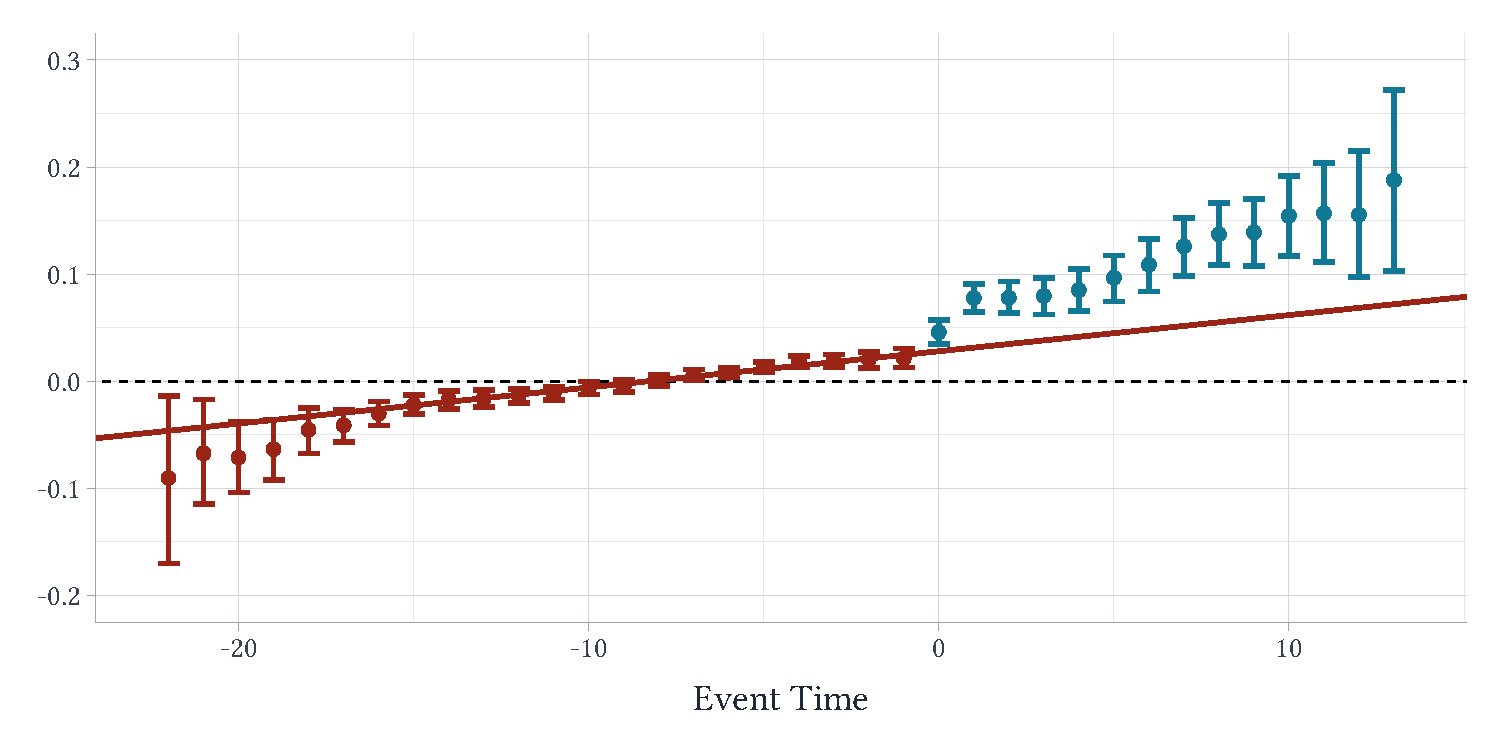
\includegraphics{figures/generalized/did2s_retail.pdf}
  \end{adjustbox}
\end{subfigure}
\end{center}
\begin{center}
\begin{subfigure}[b]{0.75\textwidth}
  \caption{Generalized Imputation Estimator}
  \begin{adjustbox}{width=\textwidth, center}
    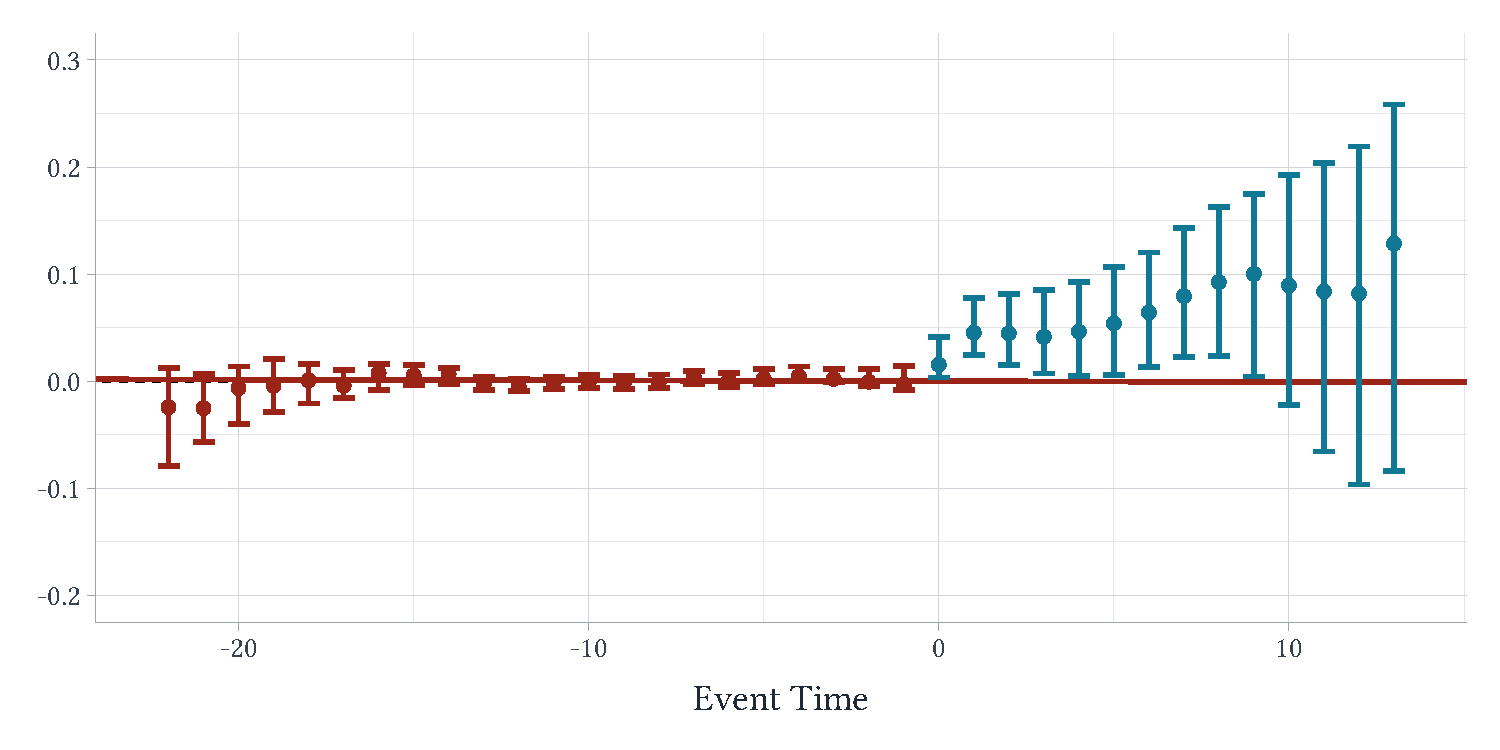
\includegraphics{figures/generalized/qld_retail.pdf}
  \end{adjustbox}
\end{subfigure}
\end{center}

\note{This figure plots point estimates and bootstrapped 95\%  confidence intervals for event-study treatment effects on $\log$ retail employment. Panel (a) estimates effects using the TWFE imputation estimator proposed in \citet{Borusyak_Jaravel_Spiess_2021}. Panel (b) estimates effects using the generalized imputation estimator we propose in Section \ref{sec:estimation} with $p = 2$ and using the following instruments: 1980 share of population employed in manufacturing, 1980 shares of population below and above poverty line; 1980 shares of population employed in private-sector and by the government, 1980 shares of population with high-school degree and college degree. The red lines correspond to a linear estimate of pre-treatment point estimates for event time -15 to -1 and is extended into the post-treatment periods.}
\end{figure}

We use the QLD estimator of \citet{Ahn_Lee_Schmidt_2013} to estimate the factors as described in remark \ref{remark:QLD}. For this factor estimator, we need a set of instruments that satisfy the two standard instrument requirements: relevancy and exclusion. Intuitively, the relevancy restriction requires that the instruments are correlated with the full vector of factor-loadings. That is, the instruments should be selected as `proxies' for the kinds of economic factor-loadings that the researcher is concerned of. The exclusion restriction requires that the instrument values are uncorrelated with location-specific idiosyncratic shocks. For this reason, we use baseline covariate values as instruments to avoid shocks to the covariates that are correlated with shocks to the outcome variable. 

We select instruments that we suspect are driven by the general macroeconomic trends that cause differential retail employment growth in the 1980s and 1990s. For example, retail employment is likely driven by consumptive expenditures which in turn are reflective of local labor market trends. Therefore, we use instruments that we think proxy for characteristics that determine local labor market trends. Specifically, we use the 1980 baseline values of the following variables as instruments: share of population employed in manufacturing, shares of population below and above the poverty line; shares of population employed in the private-sector and by the government, and shares of population with high-school and college degrees.\footnote{All of these values are obtained from 1980 Census Tables accessed from \citet{manson2020ipums}.} We use baseline shares to prevent our instruments from picking up on contemporaneous economic shocks that could be correlated with Walmart opening, i.e. to avoid violations of the exclusion restriction. Note that instead of estimating $\ATT(g,t)$, we estimate $\ATT^\ell$ pooling across $(i, t)$ with $\ell = t - g_i$ as described after Theorem \ref{theorem:asymptotic_distribution}.

\begin{figure}
\caption{Effect of Walmart on County $\log$ wholesale Employment}
\label{fig:walmart_wholesale}

\begin{center}
\begin{subfigure}[b]{0.75\textwidth}
  \caption{TWFE Imputation Estimator}
  \begin{adjustbox}{width=\textwidth, center}
    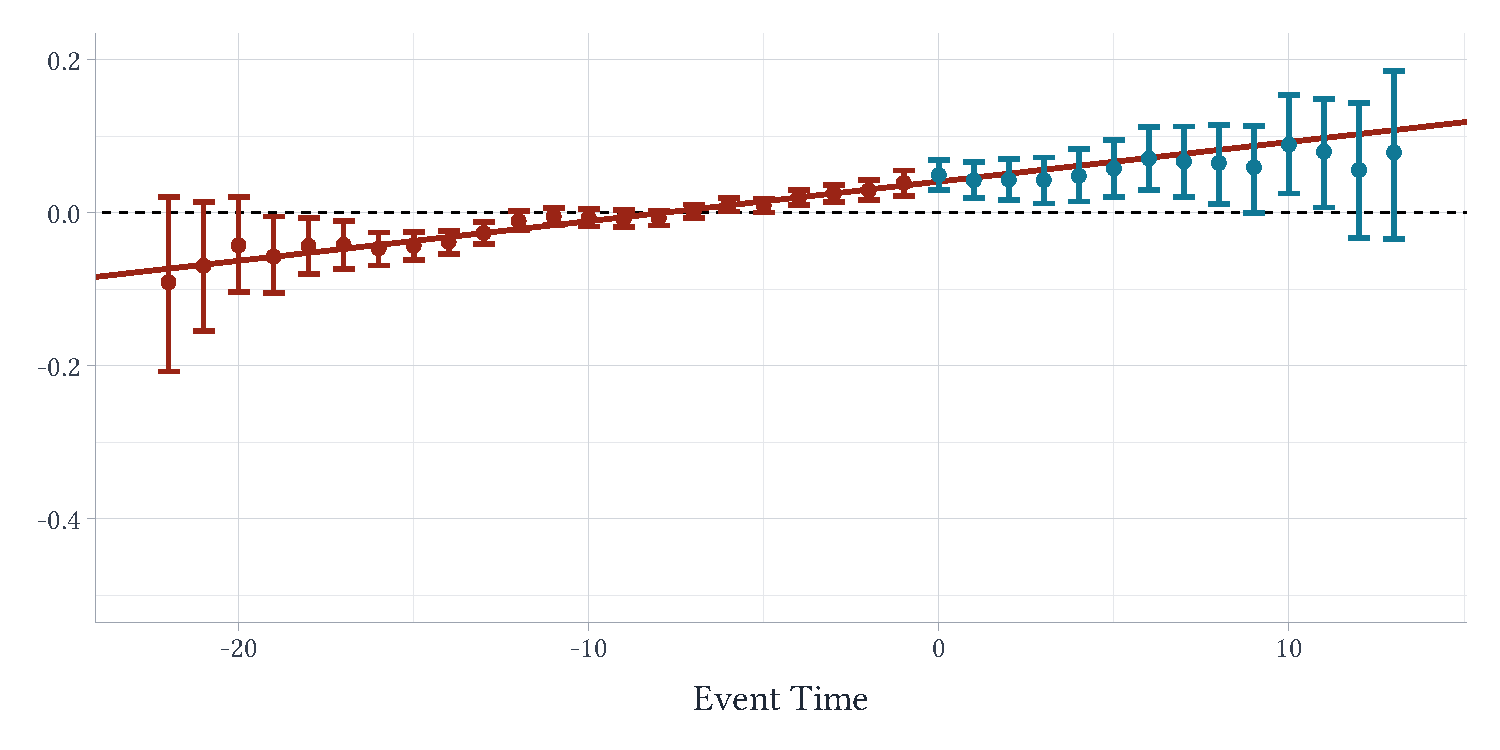
\includegraphics{figures/generalized/did2s_wholesale.pdf}
  \end{adjustbox}
\end{subfigure}
\end{center}
\begin{center}
\begin{subfigure}[b]{0.75\textwidth}
  \caption{Generalized Imputation Estimator}
  \begin{adjustbox}{width=\textwidth, center}
    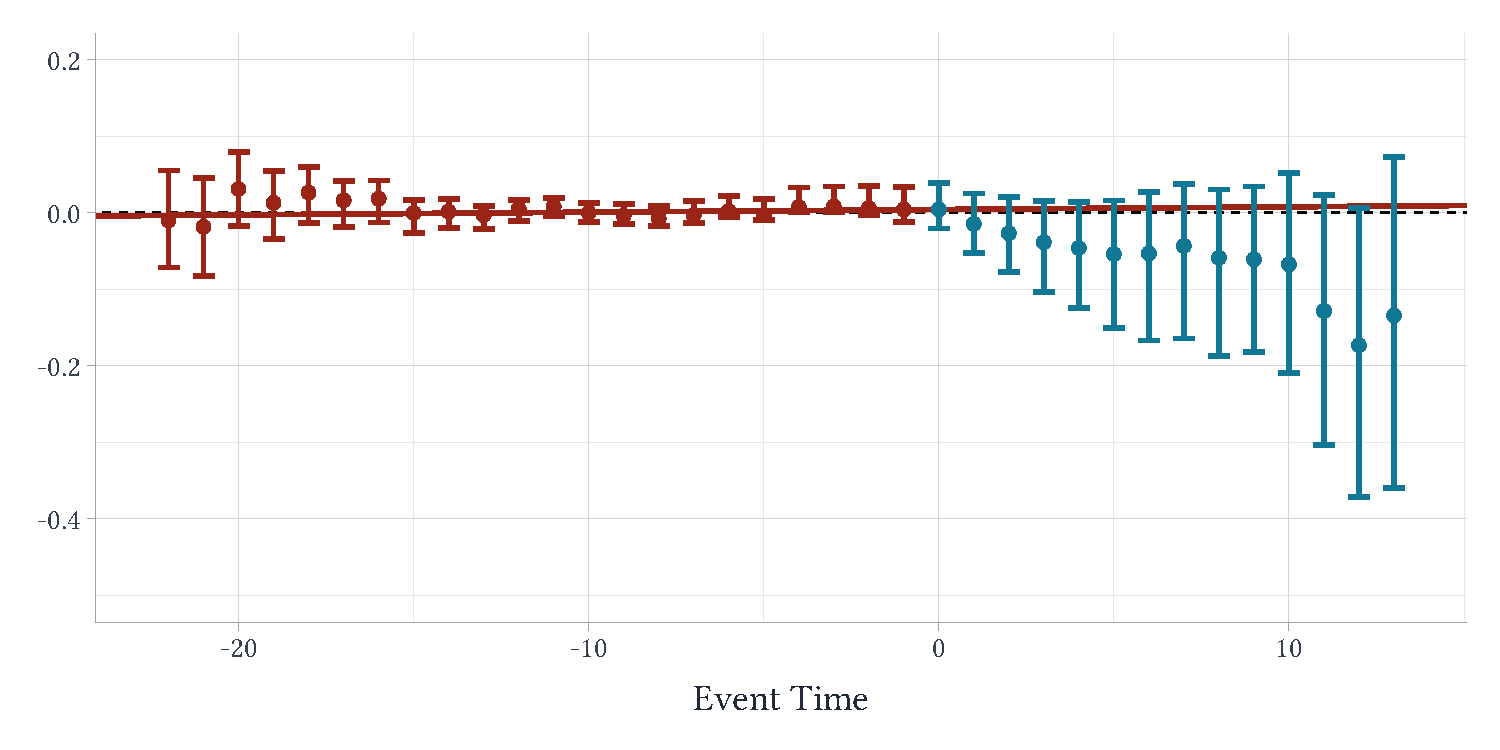
\includegraphics{figures/generalized/qld_wholesale.pdf}
  \end{adjustbox}
\end{subfigure}
\end{center}

\note{This figure plots point estimates and bootstrapped 95\% confidence intervals for event-study treatment effects on $\log$ wholesale employment. Panel (a) estimates effects using the TWFE imputation estimator proposed in \citet{Borusyak_Jaravel_Spiess_2021}. Panel (b) estimates effects using the generalized imputation estimator we propose in Section \ref{sec:estimation} with $p = 1$ and using the following instruments: 1980 share of population employed in manufacturing, 1980 shares of population below and above poverty line; 1980 shares of population employed in private-sector and by the government, 1980 shares of population with high-school degree and college degree. The red lines correspond to a linear estimate of pre-treatment point estimates for event time -15 to -1 and is extended into the post-treatment periods.}
\end{figure}

The results of our estimator are presented in panel (b) of figure \ref{fig:walmart_retail} and figure \ref{fig:walmart_wholesale}.\footnote{We carry out the test to determine the correct number of factors $p$ following the discussion in \citet{Ahn_Lee_Schmidt_2013}. For retail, the p-value of the over-identification test were as follows: p = 0 with a p-value of 1.56e-5; p = 1 with a p-value of 0.001; p = 2 with a p-value of 0.133.  Since $p = 2$ is the first value where we fail to reject the null at a 10\% level, we set $p = 2$. Similarly, we selected $p = 1$ for wholesale since the p-values were: p = 0 with a p-value of 0.049; and p = 1 with a p-value of 0.40.} For retail employment, there is basically no pre-trend violations with the pre-treatment point estimates centered on zero. After removing the pre-existing economic trends, the point estimates are smaller than estimated by the two-way error model with an estimated effect on employment of around 6\% on average in the post-treatment periods. Evaluated at the median baseline retail employment of 1417 employees, this would imply an increase in about 85 jobs, which is in line with the estimates of \citet{basker2005job} and \citet{stapp2014Walmart} who use alternative instrumental variables strategies. It is important to note that post-treatment estimates are noisier than the TWFE estimates largely due to estimating the factor proxies in the first stage. This problem is at its worst for the furthest event-times due to very few counties being averaged over in the last few bins. We view this as a worthy trade-off since the point estimates are much less likely to be biased. 

Turning to wholesale employment, we see a similar story with our estimator removing most of the pre-trend violations. In this case, however, the estimated effects flip signs with an estimated effect of around -6\%, although they are not statistically significant at the 5\% level. Evaluated at the 1977 median wholesale employment of 410, this suggests a decrease of about 25 jobs, which is similar to what \citet{basker2005job} finds. Overall, we find effects very much in line with those reported in \citet{basker2005job}.

Our estimator allows for any root-$N$ consistent estimator of the factor's column space to be `plugged-in' and used for estimation of treatment effects. To show the versatility of the method, we use three different factor estimators in figure \ref{fig:many_factor_estimators}. First, we use our original quasi-differencing estimator from figure \ref{fig:walmart_retail}. Second, we use the common correlated effects (CCE) estimator originally proposed in \citet{pesaran2006estimation}. This estimator uses a set of covariates, $\bm X$, which are generated by the same factors, $\bm{F}$, as the outcome variable:
\begin{equation}
  X_{it} = \bm\alpha_i' \bm{F}_t + \nu_{it}.
\end{equation}
Under this assumption, the cross-sectional averages of $X$ (averaged over the never-treated group) consistently span the column space of $\bm{F}$.  In our application, we use log employment for the manufacturing, construction, agriculture, and healthcare 2-digit NAICS codes. The choice of these covariates is plausible if the same sort of national shocks that affect retail employment also affect these other sectors. We more formally analyze this estimator in \citet{Brown_Butts_Westerlund_2023}, which derives the asymptotic distribution of the estimates. One advantage of this factor estimator is that it allows decomposition of treatment effects into direct effects and mediated effects that operate through the covariates, $X_{it}$.

Last, we use the principal components estimator originally proposed in \citet{Bai_2009}. This estimator uses the eigenvectors  of the matrix $\bm Y \bm Y'$ with the $p$ largest eigenvalues as estimates for $\bm{F}$.\footnote{This imputation estimator is proposed by \citet{Xu_2017} in the context of large panels. The author uses an alternative identification strategy that fails to work in short panels.} The advantage of this estimator is that no instrument or additional covariates are required. However this comes at the cost of requiring long panels, which may be infeasible to assume in our application.

\begin{figure}
\caption{Generalized Imputation Estimator for Effect of Walmart on County Employment with Different Factor Estimators}
\label{fig:many_factor_estimators}

\begin{center}
\begin{subfigure}[b]{0.75\textwidth}
  \caption{$\log$ Retail Employment}
  \begin{adjustbox}{width=\textwidth, center}
  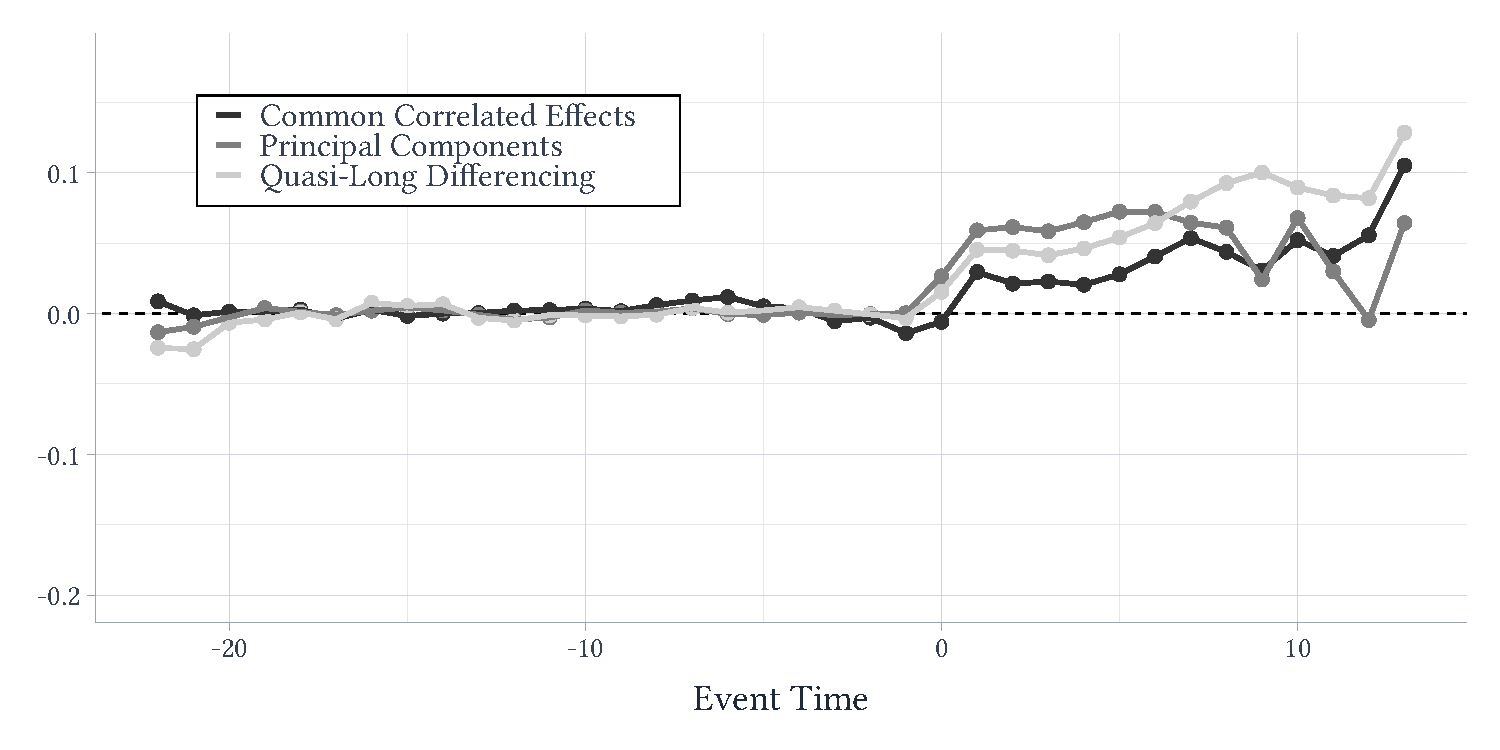
\includegraphics{figures/generalized/retail_many_estimators.pdf}
  \end{adjustbox}
\end{subfigure}
\end{center}
\begin{center}
\begin{subfigure}[b]{0.75\textwidth}
  \caption{$\log$ wholesale Employment}
  \begin{adjustbox}{width=\textwidth, center}
  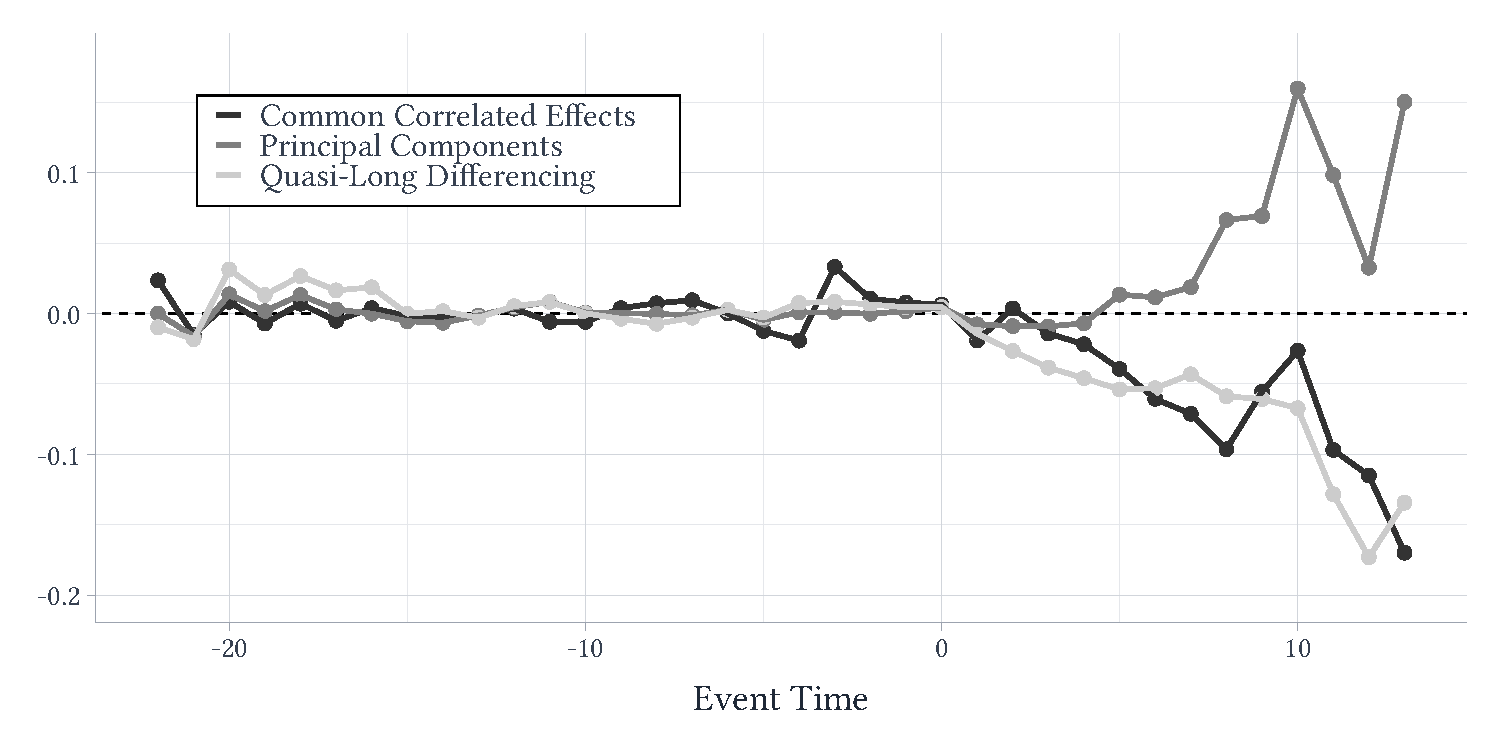
\includegraphics{figures/generalized/wholesale_many_estimators.pdf}
  \end{adjustbox}
\end{subfigure}
\end{center}

\note{This figure presents estimated treatment effects of Walmart entry on county-level $\log$ retail employment using the generalized imputation procedure proposed in section \ref{sec:ATT_identification}. The factor estimation procedures include the principal components estimator proposed in \citet{Bai_2009}, the common correlated effects estimator proposed in \citet{pesaran2006estimation}, and the quasi-differencing estimator proposed in \citet{Ahn_Lee_Schmidt_2013}. Details of the estimation procedures appear in the text.}
\end{figure}

The results of each estimator are presented in figure \ref{fig:many_factor_estimators}. All three estimators are effective at removing underlying trends that the treated counties experienced. Moreover, the estimated effects are similar between estimators suggesting that all three are doing a good job at estimating the underlying factors. This figure highlights the broad applicability of our identification results, allowing the factor estimator of choice to be tailored to the research context at hand. In panel (b), we use $\log$ wholesale employment as an outcome. The CCE and the quasi-differencing estimators produce very similar results, while the principal components estimator suggests positive growth in employment outcomes in later years. Corresponding confidence intervals are very large, suggesting that these results are too noisy to draw any meaningful conclusions. This could be due to wholesale employment being too auto-correlated for the factor estimates to be consistent, or because we do not have a large enough time series to get a meaningful asymptotic approximation of the factors.

% As we discuss above, one reason the synthetic control literature is increasingly popular is that it allows researchers to transparently plot the counterfactual estimates of $y(0)$ for the treated unit. For this reason, we plot the observed $\tilde{y}_{it}$ and the imputed $\hat{\tilde{y}}_{it}(0)$ for (log) retail and wholesale employment in figure \ref{fig:synthetic_control_plot}. In pre-treatment ($\ell < 0$), the imputed estimate, our `synthetic control' follows closely with the observed $\tilde{y}_{it}$ giving us confidence in our ability to approximate the factor structure. In the post-periods, we see the observed counties and the imputed untreated version of the counties pulling apart. The gap between the two are our estimated treatment effects. 
% 
% \begin{figure}
% \caption{Synthetic Control Style Plot of the Effect of Walmart on County Employment}
% \label{fig:synthetic_control_plot}
% 
% \begin{subfigure}[b]{0.49\textwidth}
%   \caption{$\log$ Retail Employment}
%   \begin{adjustbox}{width=\textwidth, center}
%     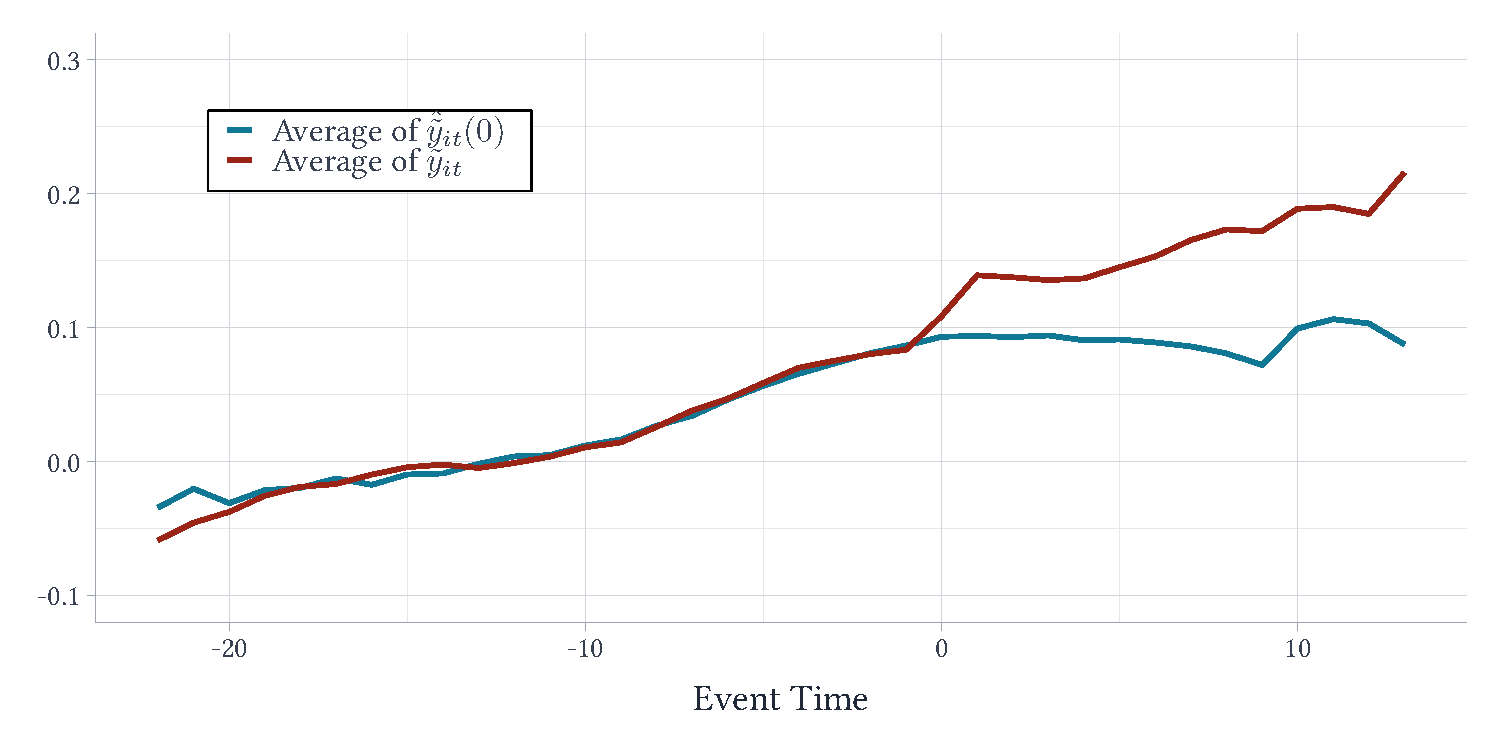
\includegraphics{figures/generalized/synth_retail.pdf}
%   \end{adjustbox}
% \end{subfigure}
% \hfill
% \begin{subfigure}[b]{0.49\textwidth}
%   \caption{$\log$ wholesale Employment}
%   \begin{adjustbox}{width=\textwidth, center}
%     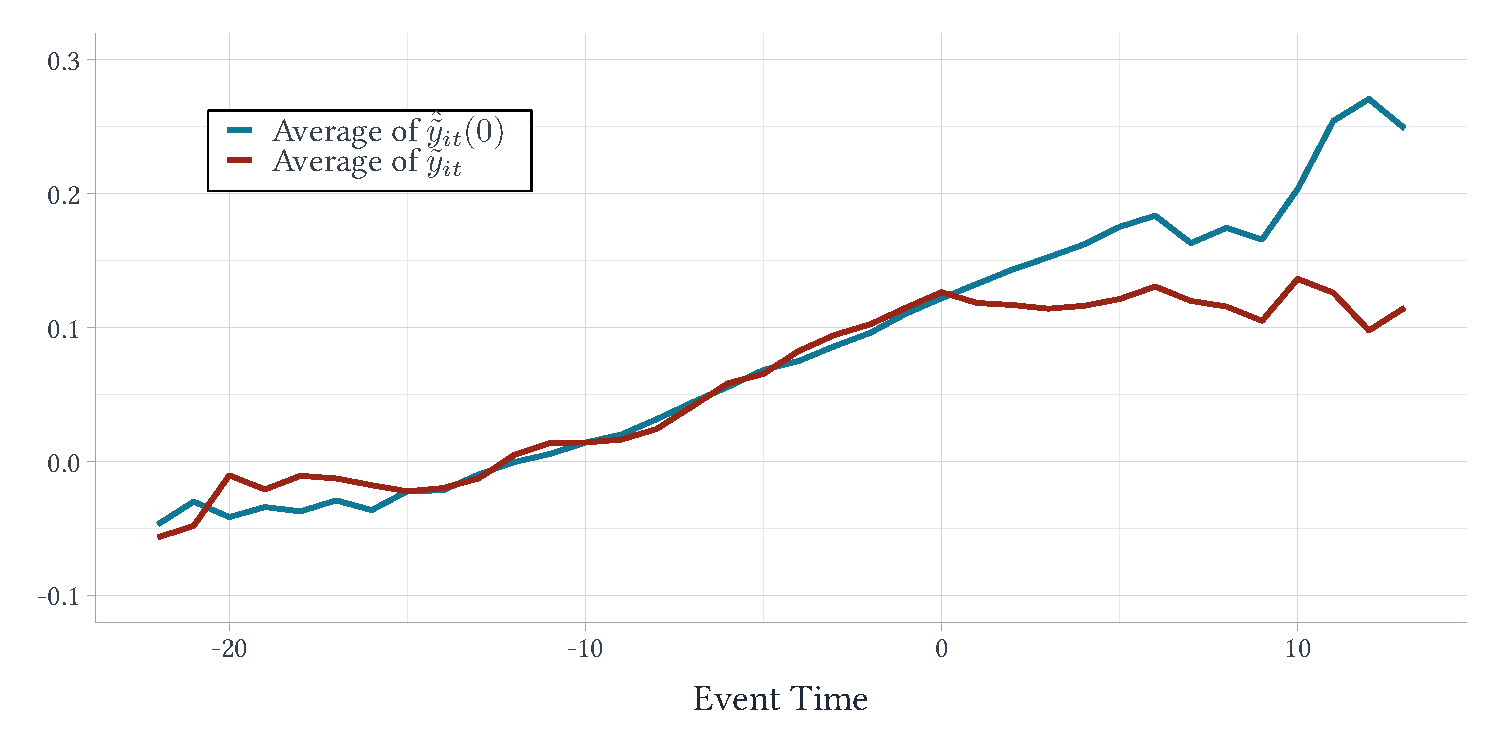
\includegraphics{figures/generalized/synth_wholesale.pdf}
%   \end{adjustbox}
% \end{subfigure}
% 
% \note{This figure plots the observed $\tilde{y}_{it}$ and the imputed $\hat{\tilde{y}}_{it}(0)$ for treated units averaged over event time $\ell = t - g_i$. We impute within-transformed potential outcome using the generalized imputation estimator we propose in Section \ref{sec:estimation} using the following instruments: 1980 share of population employed in manufacturing, 1980 shares of population below and above poverty line; 1980 shares of population employed in private-sector and by the government, 1980 shares of population with high-school degree and college degree.}
% \end{figure}

To highlight the importance of the uncertainty from estimation of the factors in the first stage, we recreate confidence intervals from our generalized imputation estimator with the QLD first stage using the nonparametric standard errors that are derived in Theorem \ref{theorem:nonparametric_variance}. Results are given in figure \ref{fig:Walmart_naive_se}. The standard errors on point estimates are far smaller, with estimates becoming strongly significant in wholesale Employment. This result shows an important step for future research in finding more efficient estimates of the factors. For instance, we consider the common correlated effects estimator in a follow-up paper. The CCE model generally implies that the nonparametric standard errors are valid when there is a common factor model for time-varying covariates.

\begin{figure}
\caption{Generalized Imputation Estimator for Effect of Walmart on County Employment with Naive Standard Errors}
\label{fig:Walmart_naive_se}

\begin{subfigure}[b]{0.49\textwidth}
  \caption{$\log$ Retail Employment}
  \begin{adjustbox}{width=\textwidth, center}
    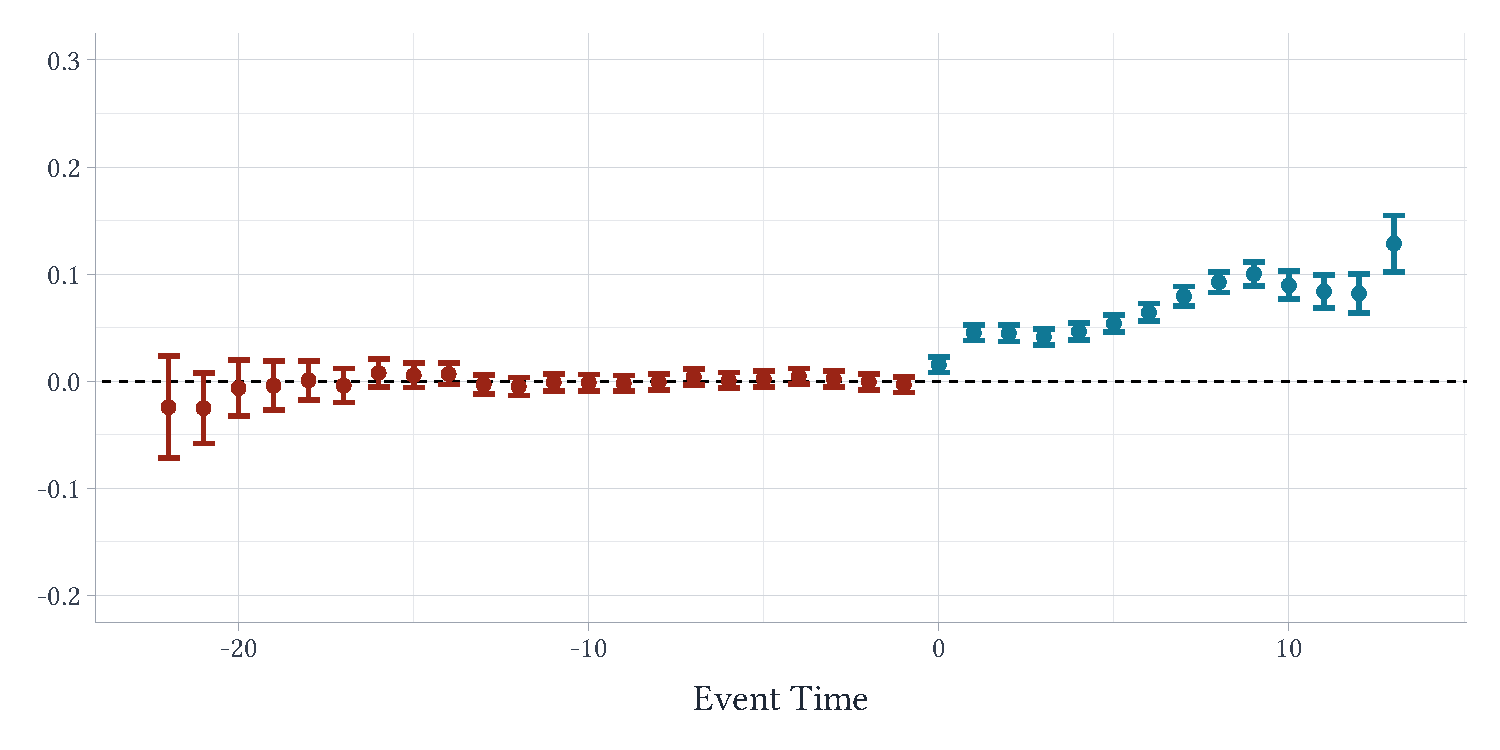
\includegraphics{figures/generalized/qld_retail_naive_se.pdf}
  \end{adjustbox}
\end{subfigure}
\hfill
\begin{subfigure}[b]{0.49\textwidth}
  \caption{$\log$ wholesale Employment}
  \begin{adjustbox}{width=\textwidth, center}
    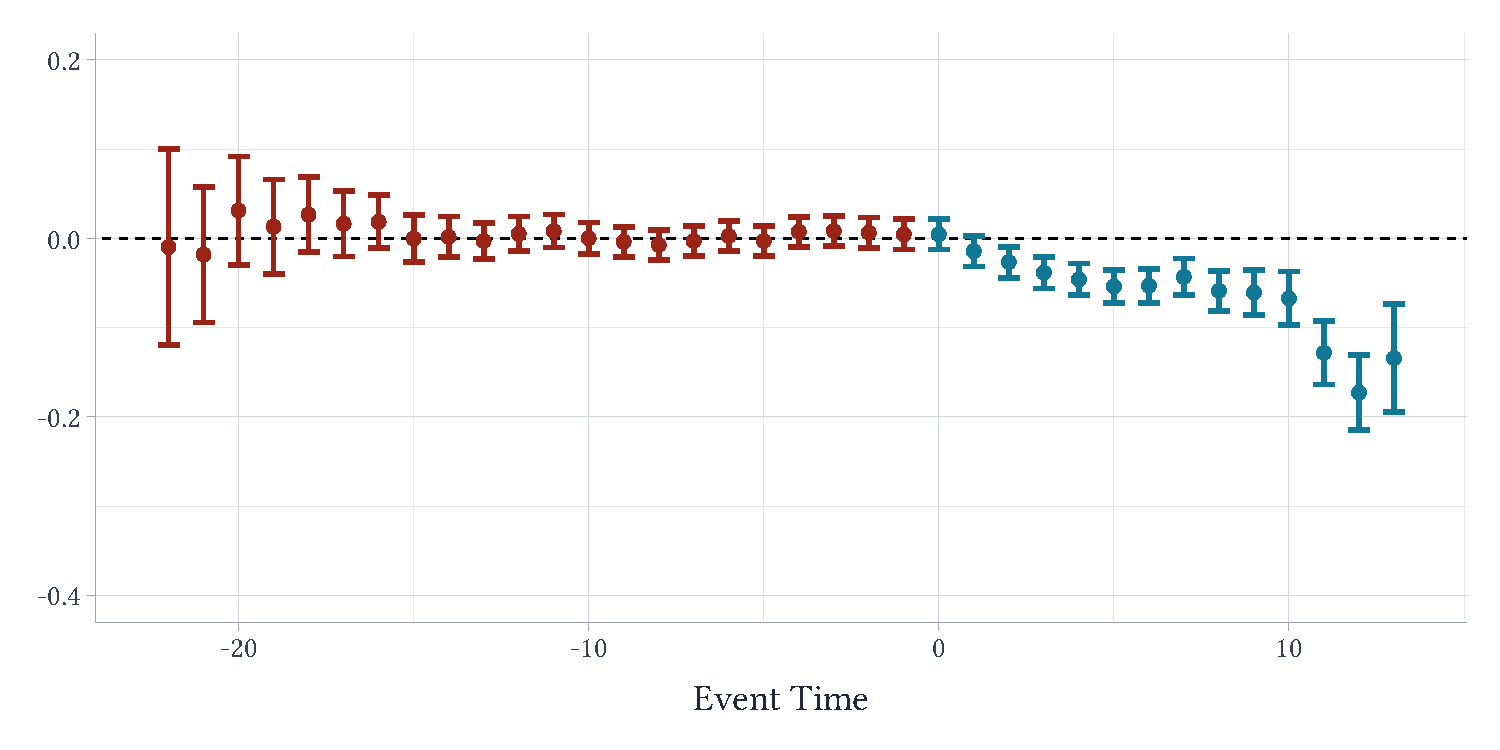
\includegraphics{figures/generalized/qld_wholesale_naive_se.pdf}
  \end{adjustbox}
\end{subfigure}

\note{This figure recreates estimates from panel (b) of figure \ref{fig:walmart_retail} and figure \ref{fig:walmart_wholesale} with confidence intervals formed ignoring the uncertainty deriving from first-stage estimates of $\theta$.}
\end{figure}


% ------------------------------------------------------------------------------
\section{Conclusions}
% ------------------------------------------------------------------------------

We consider identification and inference of functions of heterogeneous treatment effects in a linear panel data model. We show how to relax the usual parallel trends assumption by introducing a linear factor model in the error. Our main identification result shows that a consistent estimator of the unobserved factors is all that one needs to estimate the dynamic treatment effect coefficients. This result is general and can be implemented by a number of modern interactive fixed effects estimators, such as quasi-long-differencing, internally generated instruments, common correlated effects, or principal components, allowing for both large and small numbers of pre-treatment time periods. Further work can demonstrate both theoretical and finite-sample properties of these various estimators of the factors and how they affect to ATT estimation, especially for larger time series. The GMM imputation framework should also be examined in the context of unbalanced panels as in \citet{Rai_2022}. 

While a factor model nests the usual two-way error structure, we explicitly model the level fixed effects in addition to the factors. This setting allows us to provide useful tests for the consistency of the TWFE estimator. We also show that one must remove the unit and time fixed effects in a particular way so as to preserve the common factor structure in all time periods for all individuals. We provide such a transformation and prove a novel identification result for TWFE imputation estimators of ATTs.

We implement the QLD estimator of \citet{Ahn_Lee_Schmidt_2013} in a study of the local impact of Walmart openings. We demonstrate findings consistent with the IV estimation strategy of \citet{basker2005job}.  Our estimator is shown to remove pre-trends that bias the usual TWFE estimates. Similar results are found using common correlated effects in the first stage. A principal components estimator is also explored, but performs suspiciously for the given problem. The QLD identification scheme can also allow sequentially exogenous outcomes like those generated by dynamic models. We leave this possibility for future study. 

\chapter{Difference-in-Differences with Spatial Spillovers}

% ------------------------------------------------------------------------------
\section{Introduction}
% ------------------------------------------------------------------------------

Empirical work in economics often considers settings where a policy targets units grouped by geographic boundaries but the effect of treatment spills over onto `nearby' units.\footnote{The framework of this paper applies to any setting with a well-defined measure of distance, e.g. geographic distance, economic distance such as supply chains, node distance in a graph, or social relationships in schools or cities.} For example, individuals in the surrounding area can travel across borders to receive treatment (e.g. a new  hospital serves nearby residents); or shocks to a labor market can affect nearby areas (e.g. a new factory increases service sector spending in the entire commuting zone). In these settings, a common approach involves using a structural model to account and control for general equilibrium effects. For example, trade models generate a market access term that effectively controls for such effects \citep{Donaldson_Hornbeck_2016}, or network models suggest a linear-in-means model controlling for the average characteristics of a unit's peers, e.g. proportion of peers treated \citep{manski1993identification,goldsmith2013social,Miguel_Kremer_2004}. 

However, researchers often wish to remain agnostic to structural assumptions, preferring minimal and transparent restrictions that, when made, allow for identification of treatment effects. This paper uses the potential outcomes framework proposed by \citet{vazquez2023identification} to consider non-parametric identification in difference-in-differences settings under the presence of spatial spillovers. In this framework, potential outcomes are now characterized by a unit's treatment status as well as the `exposure' to the treatment status of other units. Identification arguments are then made by imposing assumptions on the potential outcomes. 

Under the more general potential outcome framework, there are many potential treatment effects that can be formed. I consider identification of two relevant treatment effects that are common in the literature on interference \citep{savje2021average}. First, there is the `switching effect' which is the relevant parameter for local policymakers who want to answer, ``What is the effect of switching my treatment status, holding fixed all other units' treatment?''. I show that identification of the switching effect is a difficult problem which in a difference-in-differences framework would require the researcher to identify treated and control units that have the same level of exposure.\footnote{\citet{xu2023difference} takes this approach and discusses estimation and inference about this estimate.} 

The second effect of interest is the `total effect', which is the relevant parameter for national policymakers who want to answer, ``What is the average effect of implementing the entire treatment regime?''. This treatment effect is useful in post-hoc analyses analyzing the effect of implementing the observed treatment vector. This paper identifies simple and interpretable assumptions that allow for identification of the total effect. In settings where researchers are willing to impose an assumption that spillovers are `local', i.e. spillovers only impact units within a certain distance of treatment, I show the total effect can be identified with a parallel trends assumptions between treated and non-affected `far-away' units. The local spillovers assumption is reasonable in settings where travel is the primary driver of spillovers (e.g. people in nearby jurisdictions travel to the treated location). However, this assumption may not hold in the case of large general equilibrium shocks that affect units far away from the treatment area, such as when New York's economy impacts San Francisco.

In this framework, I evaluate common practices in empirical work. First, I show that the standard difference-in-differences estimator produces biased estimates for the total effect. This bias arises from the fact that untreated units that are "close" to treated units experience treatment effects, thereby failing to identify the counterfactual trend. The difference-in-differences estimate averages the spillover onto the "close" control units into the untreated units' change in outcomes. As a result, the spillover is subtracted from the estimated treatment effect, introducing bias in the opposite sign of the spillover effect. 

This problem is generally well understood, and it is common to either drop or include a dummy for nearby units in the standard two-way fixed effect model. This method consistently estimates the total effect under the assumptions I present in this paper. In this sense, this paper formalizes and clarifies the assumptions needed for this method. 

To show the importance of considering spillover effects and the utility of my estimators, I revisit analyses of place-based policies in urban economics in section \ref{sec:tva}. I revisit the analysis of the Tennessee Valley Authority by \citet{Kline_Moretti_2014a}. The Tennessee Valley Authority was a large-scale New Deal program that lowered the cost of power for industrial firms \citep{Kitchens_2014}. The scale of federal investment in the region was large and the pro-manufacturing benefits likely spread further than the Authority's boundary due to the electrification infrastructure and agglomeration economies \citep{severnini2023power}. I show that estimation by difference-in-differences fails to account for these spillovers and therefore the authors obtain biased estimates of the total effect of the Tennessee Valley Authority. For agriculture employment, I find that the long-run spillovers cause the original estimates to be about 40 percent too small for agriculture employment and 40 percent too large for manufacturing employment. 
% Following this empirical application, I briefly discuss how my framework fits into a larger discussion on identification strategies with place-based policies.
% (-0.0739 - -0.0514) / (-0.0514) = 43.7\% increase
% (0.0350 - 0.0560) / (0.0560) = 37.5\% decrease

Last, in section \ref{sec:event_study}, I extend estimation of treatment and spillover effects into settings with staggered-treatment timing by extending the work of \citet{Gardner_2021,Borusyak_Jaravel_Spiess_2021}.\footnote{I also briefly discuss how to adapt the estimation strategy of \citep{Callaway_SantAnna_2020}.} The proposed two-stage estimator first estimates unit and time fixed-effects using untreated/not-yet-treated observations. Since some control/not-yet-treated units can be affected by spillovers, these units must be removed to consistently estimate the unit and time fixed-effects. Then these estimated unit and time fixed-effects are subtracted from the observed outcome \textit{in the full sample}. The resulting differenced outcomes are then regressed on the treatment and spillover variables to estimate treatment and spillover effects. In the appendix, I demonstrate the method by revisiting the analysis by \citet{Bailey_Goodman_Bacon_2015} of Community Health Centers which provided low-cost primary care to impoverished areas.

This paper contributes to the literature that focuses on estimation of treatment effects with spatial spillovers using the difference-in-differences framework. Most work derives results for specific spillover mappings \citep{Clarke_2017,Berg_Streitz_2019,veribtsky2021causal,Delgado_Florax_2015}. My paper is the first to consider non-parametric identification in terms of general potential outcomes. My paper also advances the literature by considering estimation of treatment effects and spillover effects in settings with staggered-treatment timing. If I assume the particular functional forms for potential outcomes, I arrive at the same bias equation as theirs. \citet{xu2023difference} complements this paper well, focusing on identification and inference on the `switching effect'. 

This paper relates to a broad literature on spillover effect estimation in randomized experiments.\footnote{See \citet{sobel2006randomized} and \citet{Hudgens_Halloran_2008} for early work. See \citet{Hu_Li_Wager_2021}, \citet{savje2021average}, and \citet{vazquez2023identification} and references therein for recent work on this.} There are two main strands of this literature. First, there is a large literature on the estimation of treatment effects in the presence of spillovers using a `partial identification' framework where units are in distinct treatment clusters and outcomes depend on the treatment status within the observation's cluster only.\footnote{ \citet{Angelucci_DiMaro_2016} provides an overview of estimation of treatment effects in the presence of ``within-group'' spillovers. Empirical examples include \citet{Halloran_Struchiner_1995,sobel2006randomized,Miguel_Kremer_2004,Angrist_2014}.} Estimation compares units in the partially treated clusters with control units in completely untreated clusters which do not receive spillover effects. This allows standard difference-in-differences estimation of both the total effect (treatment effect on the treated) and spillover effects (treatment effect on the untreated in the treated clusters). However, my proposed estimator focuses on a setting without distinct clusters.

There is also a nascent literature exploring estimation of treatment and spillover effects which does not require a completely untreated cluster in experimental settings (\citet{savje2021average}; \citet{vazquez2023identification}; \citet{Hu_Li_Wager_2021}; \citet{yu2022estimating}). Those papers' identification results rely on \textit{design-based} assumptions around the treatment-assignment mechanism. Difference-in-differences, however, relies on \textit{model-based} assumptions on the potential outcomes (i.e. parallel-trends assumption) for identification in non-experimental settings. I contribute to this literature by formalizing identification results of different treatment effects in non-experimental settings. \citet{wang2020design} consider estimation of treatment effects in spatial settings under design-based settings and make a similar `local' spillovers assumption as this paper. 


% ------------------------------------------------------------------------------
\section{Theory}
% ------------------------------------------------------------------------------

There are a set of units $i \in \{1, \dots, N\}$ observed for periods $t \in \{0,1\}$ and treatment turns on between periods for some of the units. The framework is extended to staggered treatment adoption below. Let $D_i$ denote an indicator for unit $i$ being treated and the vector of treatment assignments as $\bm{D} = (D_1, \dots, D_n)'$. Since units can be impacted by the vector of treatment assignments, the general potential outcome notation is given by $Y_{it}(\bm{D})$. To simplify the high-dimensional set of potential outcomes, we follow \citet{aronow2017estimating,vazquez2023identification}, and introduce an `exposure mapping' which summarizes how a unit is exposed to spillovers: $h_i(\bm{D}): \{0, 1\}^N \to \mathcal{H}$ for some space $\mathcal{H}$ with $\dim(\mathcal{H}) \leq N$. For example, researchers might think $h_i(\bm{D})$ to be an indicator variable equal to one if any contiguous units are treated. The exposure mapping simplifies the potential outcome notation by imposing that if two treatment vectors $\bm{D}$ and $\tilde{\bm{D}}$ have $h_i(\bm{D}) = h_i(\tilde{\bm{D}})$, then the potential outcomes are also equal. Potential outcomes therefore can be written as $Y_{it}(D_i, h_i(\bm{D}))$. In the counterfactual world without treatment, we write the potential outcome as $Y_{it}(0, \bm{0})$ where $\bm{0} \in \mathcal{H}$ is defined as zero-exposure.

Often, researchers will try to parameterize potential outcomes, i.e. selecting a function $h_i(\cdot)$, by reasoning through the nature of the spillovers and subsequent estimation will rely on the functional form assumptions made by researchers. This paper will take an alternative approach to identification and estimation which will allow for estimation of treatment effects without requiring direct knowledge of the functional form of the exposure mapping/potential outcomes. 

Following \citet{Borusyak_Jaravel_Spiess_2021} and \citet{de2024difference}, our analysis views our panel and the treatment vector $\bm{D}$ (and hence exposure mappings) as fixed. Therefore, the uncertainty in the framework comes from stochastic potential outcomes.\footnote{See appendix section A.2 of \citet{Borusyak_Jaravel_Spiess_2021} for further discussion on fixed-design. \citet{xu2023difference} focuses on inference in a similar finite population setting.} In most of the related literature on interference, the treatment design and hence the distribution of exposure mappings is known (given $h$) so expectations can be taken without conditioning on the vector of exposure mappings.\footnote{See \citet{savje2021average} and \citet{pollmann2020causal} for discussion of estimation and inference when the treatment design is known.} The focus of this article is on difference-in-differences where identification comes from assumptions on the potential outcomes.

% ------------------------------------------------------------------------------
\subsection{Treatment and Spillover Effects}
% ------------------------------------------------------------------------------

In setups without spillovers, the treatment effect for an individual unit is well defined as $\tau_i \equiv Y_{i1}(1) - Y_{i1}(0)$. In the presence of spillovers, multiple treatment effects can be defined in this setting. This subsection will define commonly used estimands and discuss their interpretation. In the following sections, we will discuss identification strategies.

The natural analogue to the above treatment effect which I will label the `switching effect' is:
\[
  \tau_{i, switch}(\bm{h}) \equiv Y_{i1}(1, \bm{h}) - Y_{i1}(0, \bm{h}).
\] 
This is the effect of changing only unit $i$'s treatment status while keeping their exposure to spillovers constant at some value $\bm{h}$. This treatment effect is policy-relevant as it summarizes what would happen if a `local' policymakers decide to enact the policy for unit $i$ (implicitly keeping $\bm{h}$ constant).\footnote{This is what \citet{savje2021average} call the `assignment-conditional unit-level treatment effect'.} It is important to note that the switching effect can depend on the level of exposure. For instance, consider the construction of libraries in towns \citep{berkes2021knowledge}. The effect of a new library in a town that is far away from any other library (exposure of $\bm{0}$) is different than a town that is very close to a neighboring town's library (large $\bm{h}$), hence the dependence of $\tau_{i, switch}$ on $\bm{h}$. Since the size of the switching effect depends on a unit's exposure level, we will consider an average switching effect at each value of exposure, 
\[
  \tau_{\text{switch}}(\tilde{\bm{h}}) \equiv 
  \expec{Y_{i1}\big( 1, \tilde{\bm{h}} \big) - Y_{i1}\big( 0, \tilde{\bm{h}} \big)}{D_i = 1, h_i(\bm{D}) = \tilde{\bm{h}}}.
\]

The second policy-relevant parameter is the `total effect`: 
\[
  \tau_{i,\text{total}} \equiv Y_{i1}(1, h_i(\bm{D})) - Y_{i1}(0, \bm{0}).
\]
As opposed to the switching effect, which keeps exposure constant, the total effect looks at turning on treatment \textit{and} going from zero exposure to $h_i(\bm{D})$ simultaneously. This can be thought of as going from the world with a \textit{complete} absence of treatment, $\bm{0}$ to the current treatment vector $\bm{D}$. Individual effects can be averaged over treated units to the `total effect of treatment on the treated': 
\[
  \tau_{\text{total}} \equiv \expec{Y_{i1}(1, h_i(\bm{D})) - Y_{i1}(0, \bm{0}) \ \vert \ D_i = 1}.
\]
This treatment effect is helpful for `national' policymakers to evaluate what \textit{were} the effects of the entire vector of \textit{enacted policies}.\footnote{\citet{yu2022estimating} label the `total effect' to be $\expec{Y_{i1}(1, h_i(\bm{D})) - Y_{i1}(0, \bm{0})}$ where the average is over all units including control units. Identification of this effect relies on assumptions about experimental-design so this paper does not pursuit identification of this effect.} 

We formalize the `spillover effect' as the difference in potential outcomes between being exposed to the observed spillover exposure and not being exposed:
\[
  \tau_{i,\text{spill}}(d) \equiv Y_{i1}(d, h_i(\bm{D})) - Y_{i1}(d, \bm{0}).
\]
This effect can differ based on treatment status as the magnitude or even the causal mechanisms of spillovers might differ between treated and untreated units. For example, consider a targeted place-based policy that creates tax incentives to create businesses in designated census tracts. Nearby untreated census tracts could lose out on new business formation from this policy while nearby treated census tracts might benefit from agglomeration forces from a cluster of designated tracts. 

It is often also of interest to estimate the average spillover effects on subsets of units (e.g. all units experiencing non-zero exposure). Since it shows up in our below decomposition of the difference-in-differences estimand, we define the average spillover onto all the control units as
\[
  \tau_{\text{spill}}(0) = \expec{Y_{i1}(d, h_i(\bm{D})) - Y_{i1}(d, \bm{0})}{D_i = 0}.
\]
Estimation of spillover effects for different groups of units will be discussed in section \ref{sec:spill}.


% ------------------------------------------------------------------------------
\subsection{What Does Difference-in-Differences Estimate?}
% ------------------------------------------------------------------------------

With treatment effects properly defined, I will first derive what the standard difference-in-differences estimand identifies under a modified parallel trends assumption. 
\begin{assumption}[Parallel Counterfactual Trends]\label{assumption:parallel}
  Counterfactual trends do not depend on $D_i$:
  \[ 
    \expec{Y_{i1}(0, \bm{0}) - Y_{i0}(0, \bm{0}) \ \vert \ D_i = 1 } = 
    \expec{Y_{i1}(0, \bm{0}) - Y_{i0}(0, \bm{0}) \ \vert \ D_i = 0 }
  \]
\end{assumption}
This assumption states that in the absence of treatment and with zero exposure (not just the absence of individual $i$'s treatment), the change in potential outcomes from period 0 to 1 do not depend on treatment status. When the stable-unit treatment value assumption (SUTVA) is satisfied, all units have zero exposure and this assumption generalizes to the classic parallel counterfactual trends assumption. Second, I make the standard assumption `no anticipation' assumption that units do not adjust their actions in period $0$ from knowledge of future treatment:
\begin{assumption}[No Anticipation]\label{assumption:no-anticipation}
  $\expec{ Y_{i0}(D, \bm{h}(\bm{D})) } = \expec{ Y_{i0}(0, \bm{0}) }$.
\end{assumption}

With these assumptions, we derive what the standard difference-in-difference estimand identifies.
\begin{proposition}[Decomposition of Difference-in-Differences Estimand]\label{prop:bias}\ \\    
  If assumptions \ref{assumption:parallel} and \ref{assumption:no-anticipation}, the population difference-in-differences estimand can be decomposed as follows:
  \begin{align}\label{eq:did} 
      &\expec{Y_{i1} - Y_{i0}}{D_i = 1} - \expec{Y_{i1} - Y_{i0}}{D_i = 0}= \tau_{\text{total}} - \tau_{\text{spill}}(0)
  \end{align}
\end{proposition}
The proof is given in Appendix \ref{sec:spillover-proofs}, but the intuition is as follows. The change in outcomes among control units includes both the parallel counterfactual trend and the average spillover effect onto control units. Since $\hat{\tau}$ is found by subtracting the change in outcomes among the control units, we subtract the average spillover effect onto the control, $\tau_{\text{spill}}(0)$. 

% ------------------------------------------------------------------------------
\subsection{Identification of Treatment Effects}\label{sec:remove_bias}
% ------------------------------------------------------------------------------

% ------------------------------------------------------------------------------
\subsubsection{Switching Effect}
% ------------------------------------------------------------------------------

It is difficult to identify the switching effect in general as identifying the unobserved counterfactual outcome $Y_{i1}(0, h_i(\bm{D}))$ requires knowledge of which control units have the same level of exposure. The reason for this can be seen by rewriting this in terms of a difference-in-differences style estimand:
\begin{align*}
    \tau_{\text{switch}}(\tilde{\bm{h}}) &= \expec{Y_{i1}(1, \tilde{\bm{h}}) - Y_{i0}(0,\bm{0})}{D_i = 1, \bm{h}(\bm{D}) = \tilde{\bm{h}}} \\ 
    &\quad\quad - \expec{Y_{i1}(0, \tilde{\bm{h}}) - Y_{i0}(0,\bm{0})}{D_i = 1, \bm{h}(\bm{D}) = \tilde{\bm{h}} }.
\end{align*}
The first term is identified by the observed outcomes of the treated units. The second term would typically be estimated using the control units with exposure $\tilde{\bm{h}}$ under a parallel trend assumption. This is difficult as it requires knowledge of the unobserved exposure mapping to identify control units with $h_i(\bm{D}) = \tilde{\bm{h}}$. In related work, \citet{xu2023difference} take the approach of parameterizing the exposure mapping and discusses doubly-robust estimates of the switching effect.

Since spillover effects show up in the second term, estimation of the average switching effect requires an additional assumption that spillover effects on the control units be on average the same as the treated units. As an example, this assumption could fail if units that would receive the largest negative spillover effects select into treatment to avoid them. The problem of effects showing up in the above decomposition is similar to those highlighted by \citet{Callaway_Goodman-Bacon_SantAnna_2021} for difference-in-differences with continuous treatment. See their discussion on `strong parallel trends'

% \begin{assumption}[Switching Effect Parallel Trends]\label{assumption:parallel-switching}
%   For a given exposure, $\tilde{\bm{h}}$, counterfactual trends do not depend on $D$:
%   \[ 
%     \expec{Y_{i1}(0, \tilde{\bm{h}}) - Y_{i0}(0, \bm{0}) \ \vert \ D_i = 1, h_i(\bm{D}) = \tilde{\bm{h}} } = 
%     \expec{Y_{i1}(0, \tilde{\bm{h}}) - Y_{i0}(0, \bm{0}) \ \vert \ D_i = 0, h_i(\bm{D}) = \tilde{\bm{h}} }
%   \]
% \end{assumption}

% This assumption requires parallel trends among treated and control units at exposure $\tilde{\bm{h}}$. Under this assumption, the switching effect can be identified by a difference-in-differences estimand calculated using only units with an exposure of $\tilde{\bm{h}}$.

\begin{remark}
  Researchers may be tempted to introduce the parameterized exposure mapping interacted with a post dummy variable linearly in a two-way fixed effects model to ``compare individuals at the same level $\bm{h}$''. However, this assumes additive separability between the treatment dummy and the exposure mapping imposing homogeneity of switching effects for treated and untreated units. If the exposure mapping is continuous, then this also imposes switching effect grows linearly with $\bm{h}$. An alternative would be running difference-in-differences on subsets of treated and control units with the same value of $\bm{h}$. 
\end{remark}

% ------------------------------------------------------------------------------
\subsubsection{Total Effect}
% ------------------------------------------------------------------------------

To identify the total effect, additional assumptions on the nature of spillover effects are needed. In particular, I will formalize the idea that spillovers are `local' in that units are only affected by treatment if they are near treatment. For example, if treatment has to be accessed in person (e.g. access to abortion clinics), then it is natural that further away places are not affected by treatment. However, this assumption may fail under general equilibrium shocks that do not necessarily decay over distance. 

To formalize this assumption, let $d(i,j)$ be a function that measures the distance between units $i$ and $j$.\footnote{
  While the prose generally focuses on geographic distance, this could be any reasonable metric. For example, a measure of the connectedness between businesses where we assume larger values are more distant firms.
} 
For a given distance $\bar{d}$, let $S_{i}(\bar{d}) = \min_{j: \ D_j = 1} d(i,j) \leq \bar{d}$ be an indicator equal to one if unit $i$ is within $\bar{d}$ miles of the closest treated unit.
\begin{assumption}[Spillovers Are Local]\label{assumption:local}
  There exists a distance $\bar{d}$ such that 
  
  (i) For all units $i$,
  \[ 
      S_i(\bar{d}) = 0 \implies h_i(\bm{D}) = \bm{0}. 
  \]

  (ii) There exists treated and control units with $S_i(\bar{d}) = 0$.
\end{assumption}

Part (i) of assumption (\ref{assumption:local}) requires that spillovers are `local' in that units are no longer exposed to spillovers after some maximum distance $\bar{d}$. Part (ii) of Assumption (\ref{assumption:local}) requires that there exists control and treated units with no exposure. This assumption is far less strict than the identifying assumption for the switching effect in that we only need to identify which units have non-zero exposure and don't need to parameterize the exposure mapping any further.

The intuition behind identifying the total effect requires that we use control units experiencing no spillover effects to identify the counterfactual trend. However, this changes the necessary parallel trends assumption:
\begin{assumption}[Total Effect Parallel Trends]\label{assumption:parallel-mod}
  For a given $\bar{d}$, counterfactual trends are equal for the treated group and the far-away control group:
  $$
      \expec{Y_{i1}(0, \bm{0}) - Y_{i0}(0, \bm{0}) \ \vert \ D_i = 1}= 
      \expec{Y_{i1}(0, \bm{0}) - Y_{i0}(0, \bm{0}) \ \vert \ D_i = 0, S_i(\bar{d}) = 0}
  $$
\end{assumption}
With this assumption, we have the following identification result for the total effects:
\begin{proposition}[Identification of Total Effects]\label{prop:total_effect}
  Suppose that assumptions \ref{assumption:no-anticipation}, \ref{assumption:local}, and \ref{assumption:parallel-mod} hold. Then,
  \begin{equation}\label{eq:id_total}
    \tau_{\text{total}} = \expec{Y_{i1} - Y_{i0} \ \vert \ D_i = 1} - \expec{Y_{i1} - Y_{i0} \ \vert \ D_i = 0, S_i =0}.
  \end{equation}
\end{proposition}

Proofs are given in Appendix \ref{sec:spillover-proofs}. This proposition shows that if a researcher believes that spillover effects are `local', then estimation of the total effect on treated units only requires identifying which units are exposed to spillovers. The identifying assumption is that the control units are a valid comparison group \textit{after} removing the (potentially) exposed units. To estimate the total effect, we could replace the terms in proposition \ref{prop:total_effect} with their sample analogs.

\begin{remark}[Far-away control units and parallel trends]
  It is worth remarking on \nameref{assumption:parallel-mod} in terms of applied work. Often, researchers use only a subsample of observations that are close to treated observations. The idea is that if unobservable confounders evolve smoothly over space, then close units are more likely to be on similar counterfactual trends than units that are further away. The identification result and its corresponding estimator are formed by using further away units (i.e. units with $S_i = 0$). In this case, if parallel trends only hold for nearby control units, then focusing on further away units can fix the spillover bias but introduce bias from non-parallel trends. See appendix section \ref{sec:oz} for further discussion and an empirical example evaluating the 2017 U.S. Opportunity Zones using different identification strategies.
\end{remark}

\begin{remark}[Selection of $\bar{d}$]
  A natural question is why wouldn't researchers make the distance large to guarantee they have an unbiased estimate of $\tau_{\text{total}}$? Equation (\ref{eq:id_total}) should make this problem clear. Since these estimates rely on averages among units with $S_i = 0$, as $\bar{d}$ increases, the number of units with $S_i = 0$ decreases which yields more variable estimates. On the other hand, having units that experience spillovers not included in the $S_i$ indicator will leave some bias in the estimate.\footnote{Although, spillover effects typically will grow weaker over distance and if distant units are mistakenly treated as if they have zero exposure, bias should be small.} Therefore there is a bias-variance trade-off in extending the extent of $S_i$ that should be balanced by researchers guided by their particular economic context. Additionally, each value of $\bar{d}$ corresponds to a different effective control group and hence a different parallel trends assumption, rendering comparisons across $\bar{d}$ uninformative.
\end{remark}


\subsubsection{Spillover Effects}\label{sec:spill}

This section turns to identification of averages of spillover effects. To do so, it is typical to compare nearby control units to further away units. This  requires an additional parallel trends assumption that the far-away control units and the nearby control units are on the same trends:
\begin{assumption}[Spillover Effect Parallel Trends]\label{assumption:parallel-spill}
  For a given $\bar{d}$, we have: 
  \begin{align*}
    \expec{Y_{i1}(0, \bm{0}) - Y_{i0}(0, \bm{0}) \ \vert \ D_i = 0, S_i(\bar{d}) = 1} = 
    \expec{Y_{i1}(0, \bm{0}) - Y_{i0}(0, \bm{0}) \ \vert \ D_i = 0, S_i(\bar{d}) = 0}.
  \end{align*}
\end{assumption}

In this case, comparing control units with $S_i(\bar{d}) = 1$ to far-away control units will identify the average spillover effect on control units with $S_i(\bar{d}) = 1$:
$$
\expec{ Y_{i1}(d, h_i(\bm{D})) - Y_{i1}(d, \bm{0}) }{ S_i(\bar{d}) = 1, D_i = 0}
$$

Joint estimation of the total effect on the treated and the spillover effect on the nearby control units can be done using the following regression specification on the full sample:
\begin{equation}\label{eq:twfe_spill}
  Y_{it} = \tau D_i \one_{t = 1} + \gamma_0 (1 - D_i) S_i(\bar{d}) \one_{t = 1} + \mu_i + \lambda_t + \varepsilon_{it}.
\end{equation}

Note that since some units with $S_i(\bar{d}) = 1$ may not have positive exposure ($\bm{h}_i(\vec{D}) = \bm{0}$), this is not the average spillover effect for units with non-zero exposure. For example, if only units really close to treatment receive spillover effects and $S_i(\bar{d})$ contains a lot of units that experience no spillover effects, then $\hat{\tau}_{\text{spill, control}}$ could be estimated near zero even though some units experience substantial spillover effects. For example, reanalysis of \citet{linden2008estimates} in \citet{butts2023jue} finds that the arrival of sex offenders to a neighborhood has large impacts on homes within $0.05$ miles and much smaller impacts for homes between $0.05$ and $0.10$ miles. Selecting $\bar{d}$ to be $0.1$ estimated an effect that was about half as large as the estimated impact on the very close homes.

To better understand how spillover effects vary over distances, applied researchers will sometimes split up $S_i(\bar{d})$ into a set of $J$ concentric `rings' (e.g 0-20 miles, 20-40 miles, and 40-60 miles from the nearest treated unit). Equation (\ref{eq:twfe_spill}) can be modified as 
\begin{equation}\label{eq:twfe_rings}    
  y_{it} = \tau D_i \one_{t = 1} + \sum_{j=1}^J \gamma_j (1 - D_i) \text{Ring}_i^j \one_{t = 1}  + \mu_i + \lambda_t + \varepsilon_{it},
\end{equation}
where $\text{Ring}_i^j$ is an indicator for a control unit $i$ being in ring $j$ with $\sum_j \text{Ring}_{i}^j = S_i(\bar{d})$. The estimate $\hat{\tau}$ is still consistent for the total effect since the effective control group remains the same. However, interpretation of each $\hat{\gamma}_j$ as causal requires a yet stronger parallel trends assumption. Namely, units in each ring $j$ must be on the same parallel counterfactual trend as the $S_i(\bar{d}) = 0$ control group. If only assumption \ref{assumption:parallel-spill} is assumed, it is not possible separate variation in spillover effects from variation in counterfactual trends across rings. \citet{butts2023jue} shows that in some settings where you are willing to assume that parallel trends holds for all distances from treatment, a non-parametric estimator is available for average spillover effects as a function of distance. This assumption is more likely in very local settings where units do not vary in terms of temporal shocks.

% ------------------------------------------------------------------------------
\section{Applications in Place-Based Policy Analysis}
% ------------------------------------------------------------------------------

More generally, my framework provides important insights into identification strategies when analyzing the effects of place-based policies. There are two ways I contribute. First, \citet{Baum-Snow_Ferreira_2015} recognize the problem of spatial spillovers causing problems in identification and point to aggregation of units as a way to alleviate the problem (e.g. aggregating census tracts to metropolitan areas). However, this approach combines the treatment and spillover effects, which might each be of interest, into a singular aggregate effect. This method averages over heterogeneous effects (in magnitude or in nature) that might be of independent interest. The methods propose in this paper provide a strategy for disentangling treatment effect estimates with non-aggregated data. Subsection \ref{sec:tva} will revisit the analysis of a large-scale targeted policy on regional development. In this setting, spillover effects on nearby counties, via lost jobs, are of a very different nature than the direct impact on the targeted region and hence separate estimation if of practical interest. 

Second, my framework provides insight into different identification strategies often used in the literature. Since place-based policies are targeted to specific distressed areas, comparison units are often hard to find. Researchers have developed many identification strategies to find comparison units that are similar in terms of unobservables. First, researchers use border discontinuities to compare treated units to units just on the other side of the border. Other times, researchers compare approved applicants to narrowly rejected applicants. Both strategies aim to balance unobservables between treated and control units. A key difference in these identification strategies is the distance comparison units are from the treated area and therefore the former is more prone to bias due to spillovers than the latter. Subsection \ref{sec:oz} tries to highlight the differences in these identification strategies in the context of the U.S. Opportunity Zones created in 2017.

% ------------------------------------------------------------------------------
\subsection{The Tennessee Valley Authority}\label{sec:tva}
% ------------------------------------------------------------------------------

To illustrate the importance of accounting for spatial spillovers in the estimation of treatment effects, I revisit the analysis of the Tennessee Valley Authority (TVA) in \citet{Kline_Moretti_2014a}. The TVA program was a large-scale federal investment started in 1934 that focused on the construction of dams and transportation canals in an attempt to modernize the Tennessee Valley's economy. By the end of WWII, the TVA became the largest single power supplier in the country and significantly lowered the cost of wholesale energy for manufacturers.\footnote{More details on the program are found in \citet{Kline_Moretti_2014a}. The effects on wholesale electricity are discussed in \citet{Kitchens_2014}.} With over \$20 Billion (in 2000 dollars) spent which is hundreds of dollars transferred per person in the Authority, the impacts are very likely to extend past the authority's borders. \citet{Kline_Moretti_2014a} analyze a range of outcome variables, but I focus on agricultural and manufacturing employment. 
% Since the TVA primarily improved manufacturing industries through large-scale electrification, the authors predict that employment will grow in manufacturing and shrink in agricultural as workers switch to higher-paying manufacturing jobs. 

The analysis in \citet{Kline_Moretti_2014a} begins by comparing changes in county-level outcomes from 1940 to either 1960 (short run effects) or 2000 (long run effects) between treated counties in the Authority and control counties outside. The primary specification is
\begin{equation}\label{eq:tva}
    y_{c, t} - y_{c, 1940} = \alpha + \text{TVA}_c \tau + X_{c, 1940} \beta + (\varepsilon_{c, t} - \varepsilon_{c, 1940}),
\end{equation}
where $c$ denotes county, $\text{TVA}_c$ is an indicator variable for being in the Authority, and $y$ is a set of outcome variables (in logs).\footnote{The two-period difference-in-differences regression is equivalent to a first-difference regression. The authors use an Oaxaca-Blinder estimator on the first differences and the results of \citet{Kline_2011} show that this estimator is equivalent to a weighted difference-in-differences estimate. Their estimator does not differ much from the standard difference-in-differences results since the weights are not that different from uniform weights.} Pre-treatment control variables, $X_{c,1940}$, are included to allow for places to be on different long-term trends.\footnote{See footnote 8 in \citet{Kline_Moretti_2014a} for a full listing of control variables.} To improve the likelihood of the parallel trends assumption, they run a logistic regression to predict being in the TVA based on their set of control variables $X_{c,1940}$ and keep only observations in the top 75\% of predicted probability. The subsample produced from this exercise is presented in Figure \ref{fig:tva_sample}. 

In the paper, the authors discuss the nature of spillovers that they think can occur. For agriculture employment, the authors argue that improved wages in the TVA will draw agriculture workers out of nearby counties producing negative spillovers. For manufacturing, there are two countervailing forces \citep{Cuberes_Desmet_Rappaport_2021}. Positive spillovers from `urban access' would occur if electrification brought cheap power and agglomeration economies to the neighboring areas. The countervailing `urban shadow' would cause negative spillovers if firms chose to locate in the Authority that would have, in the absence of the program, decided to locate in nearby counties. My methodology will allow me to empirically test for these two forces in the data over time while removing their bias from the total effect estimates. 

\citet{Kline_Moretti_2014a} estimate (\ref{eq:tva}) to identify what I am calling the `total effect on the treated'. However, their point estimates compare, in part, changes in outcomes in TVA counties with changes in outcomes for neighboring counties that likely were impacted by the large-scale program. The authors do recognize the problem of spillover effects and the majority of the paper uses structural models to estimate the general equilibrium effects of the TVA. In this light, the re-analysis here is complementary to their work. 

% Figure: TVA Effective Sample and Spillover Variables
\begin{figure}[tb!]
    \caption{TVA Effective Sample and Spillover Variables}
    \label{fig:tva_sample}

    {\centering
        \resizebox{\textwidth}{!}{
            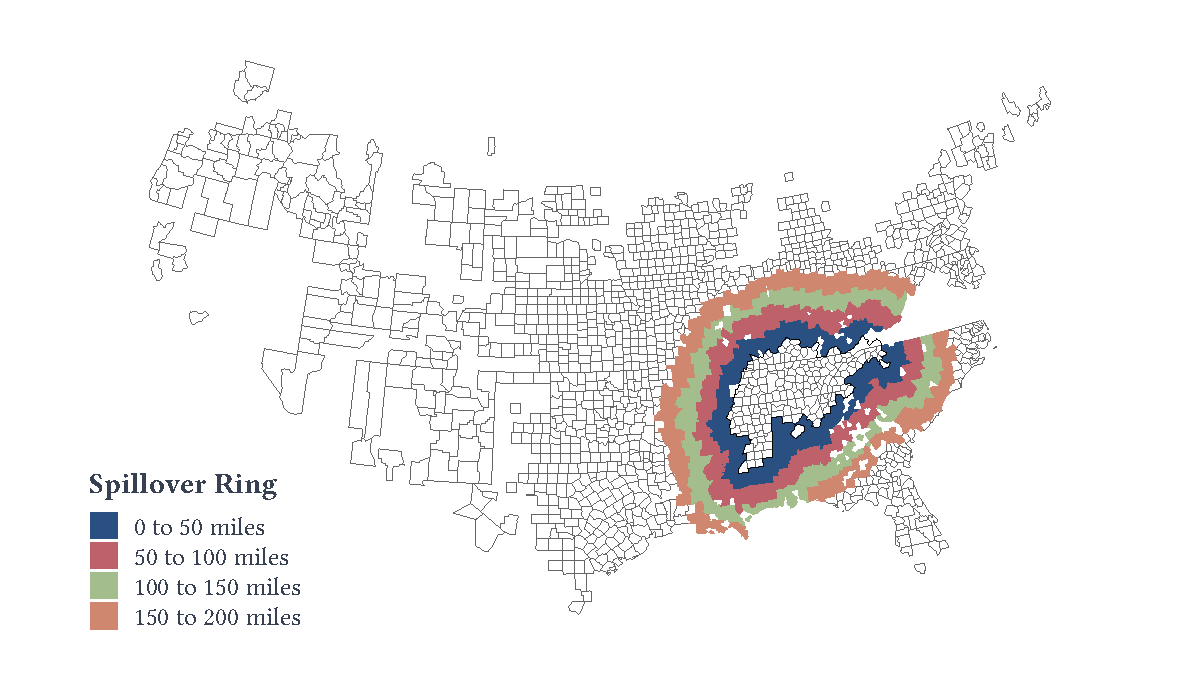
\includegraphics{figures/spatial-spillovers/tva/tva-sample.pdf}
        } 
    }
    {\footnotesize \textit{Notes:} The above figure plots all the counties used in the estimation. Counties that fall within the distance intervals $\{ (0, 50], (50, 100], (100, 150], (150, 200] \}$ measured in miles are colored by their respective bin.} 
\end{figure}

I extend their analysis to control for spatial spillovers in the difference-in-differences specification. To parameterize the exposure mapping, I use a set of rings as described in section \ref{sec:spill}. Specifically, 
the specification with spillovers is given as follows:  
\begin{equation}\label{eq:tva_spillover}
    y_{i, t} - y_{i, 1940} = \alpha + \text{TVA}_i \tau + \sum_{j \in \text{Dist}} \text{Ring}_i^j \gamma_j + X_{i, 1940} \beta + (\varepsilon_{i, t} - \varepsilon_{i, 1940}),
\end{equation} 
where $\text{Dist} = \{(0, 50], (50, 100], (100, 150], (150, 200]\}$ measured in miles and define $\text{Ring}_i^j$ as an indicator for being within the interval $d \in \text{Dist}$ away from the Authority and $t \in \{1960, 2000\}$. Figure \ref{fig:tva_sample} displays the four spillover variables by filling in each distance bin in a different color. The coefficients $\gamma_j$ estimate the average spillover effect onto control units for each of these distance bins. It's important to note that estimation of (\ref{eq:tva_spillover}) changes the comparison group to counties further away than 200 miles from the TVA.

The results of the long run analysis from 1940 to 2000 are presented in Panel A of Table \ref{tab:tva}. Each row contains the results for a different outcome variable (measured in logs). Columns (1)-(5) contain point estimates for $\tau$ and $\gamma_j$'s in different specifications. The point estimates can be interpreted as decadal growth rates in outcomes. The column labeled difference-in-differences estimates equation (\ref{eq:tva}). This estimate finds a decline in agricultural employment of about $5.1\%$ per decade and an increase in manufacturing employment of about $5.6\%$ per decade. 

% Table: Effects of Tennessee Valley Authority on Decadal Growth
\begin{table}[!tb]
  \caption{Effects of Tennessee Valley Authority on Decadal Growth}
  \label{tab:tva}
  \renewcommand{\arraystretch}{1.1}

  \begin{adjustbox}{width = \textwidth, center}
    \begin{tabular}{@{} l c@{\extracolsep{20pt}}c@{\extracolsep{4pt}}cccc @{}}
      % Head
      \toprule

      & \multicolumn{1}{c}{\textbf{Diff-in-Diff}} & \multicolumn{5}{c}{\textbf{Diff-in-Diff with Spillovers}} \\ 
      \cmidrule{2-2} \cmidrule{3-7}
      & & & TVA between & TVA between & TVA between & TVA between \\ 
      & TVA & TVA & 0-50 mi. & 50-100 mi. & 100-150 mi. & 150-200 mi. \\ 
      \textit{Dependent Var.} & (1) & (2) & (3) & (4) & (5) & (6) \\

      % Body
      \toprule
      \multicolumn{7}{l}{\textbf{Panel A:} 1940-2000} \\
      \midrule
      Agricultural employment   & $-0.0514^{***}$ & $-0.0739^{***}$ & $-0.0371^{**}$  &    $-0.0164$    & $-0.0298^{***}$ &  $-0.0157^{*}$ \\
                          &   $(0.0135)$    &   $(0.0163)$    &   $(0.0149)$    &   $(0.0114)$    &   $(0.0104)$    &   $(0.0095)$   \\
Manufacturing employment  & $0.0560^{***}$  &    $0.0350$     &    $-0.0203$    &    $-0.0245$    &    $-0.0331$    &  $-0.0296^{*}$ \\
                          &   $(0.0196)$    &   $(0.0267)$    &   $(0.0274)$    &   $(0.0338)$    &   $(0.0227)$    &   $(0.0166)$   \\


      \toprule
      \multicolumn{7}{l}{\textbf{Panel B:} 1940-1960} \\
      \midrule 
      Agricultural employment   & $0.0940^{***}$  &  $0.0856^{*}$   &    $-0.0062$    &    $-0.0042$    &    $-0.0303$    &    $-0.0039$   \\
                          &   $(0.0309)$    &   $(0.0473)$    &   $(0.0507)$    &   $(0.0487)$    &   $(0.0471)$    &   $(0.0339)$   \\
Manufacturing employment  &  $0.0894^{**}$  &  $0.0993^{**}$  &    $0.0228$     &    $0.0225$     &    $-0.0055$    &    $-0.0066$   \\
                          &   $(0.0348)$    &   $(0.0473)$    &   $(0.0554)$    &   $(0.0630)$    &   $(0.0399)$    &   $(0.0292)$   \\


      \bottomrule
    \end{tabular}
  \end{adjustbox}

  \note{
    Each row corresponds to an outcome variable. Each cell is the point estimate and the standard error for the variable described in the column title. All standard errors are Conley standard errors with a correlation cutoff of 200 miles following \citet{Conley_1999}. The column labeled `Diff-in-Diff' estimates (\ref{eq:tva}) by OLS and is similar to the estimate reported in \citet{Kline_Moretti_2014a}. The final four columns labeled `Diff-in-Diff with Spillovers' are estimates from (\ref{eq:tva_spillover}). $^{*} p< 0.1$; $^{**} p < 0.05$; $^{***} p < 0.01$.
  }

\end{table}

Turning to specification (\ref{eq:tva_spillover}) which includes spillovers, column (2) contains a point estimate for $\tau$ and columns (3)-(6) contain point estimates of the spillover effects $\gamma_j$. For agricultural employment, the point estimates show there was a decline in agriculture employment in control units near the Authority. For control units between 0 and 50 miles, column (4) indicates a decline in agricultural employment of $3.7\%$ per decade. Between 50 and 100 miles the point estimate is $-1.6\%$ per decade, between 100 and 150 miles the point estimate is $-3\%$ per decade, and between 150 and 2000 miles the point estimate is $-1.6\%$ per decade. This is likely because higher-paying manufacturing jobs within the Authority drew farm-worker migrants from nearby counties. Because the spillovers onto the control counties are negative, the original difference-in-differences estimator was positively biased. The new point estimate indicates a decline of agricultural employment of about $7.4\%$ per decade compared to $5.1\%$ in the standard difference-in-difference specification. 

For manufacturing, our point estimates for spillovers are consistently negative though imprecisely estimated. The spillover estimates suggest that neighboring counties potentially experienced negative spillover effects in the long run. Since there are negative spillover effects present, the new point estimate in column (2) of $3.5\%$ is smaller than the original estimate of $5.6\%$. The spillover estimates are evidence that in the long run, `urban shadow' (stealing manufacturing firms) forces dominate the benefits of `urban access' (agglomeration effects). 

To see how spillover effects from a large-scale place-based policy develop over time, Panel B in Table \ref{tab:tva} presents results for the effects of the Tennessee Valley in the short run using outcome data in 1960. Unlike in the long run, areas near the Tennessee Valley did not experience significant declines in agricultural employment in the short run. Since our long run analysis finds significant increases in high-paying manufacturing employment in the Tennessee Valley, this result is consistent with long run migration costs being lower than short run costs.

For manufacturing, there are potentially positive increases in manufacturing employment within 100 miles of the Tennessee Valley Authority and near-zero effects between 100 and 200 miles. In the short run, it appears that the effects of urban access and the cheap wholesale electricity dominated the effects of urban shadow. The effect of urban shadows can potentially be smaller in the short run if operating firms are unlikely to relocate. long run effects can be larger as entrant firms change their location decision and operating firms are slowly replaced which is what the long run spillover effect estimates suggest.

These results show that including spillovers in the estimation of treatment effects is potentially important and can lead to \textit{significant} differences in treatment effect estimates. Analysis of place-based policies that do not account for the fact that treatment effects can spill beyond the borders of treated areas can potentially be biased. More, the results suggest that the spillover effects caused by place-based policies change over time as frictions can create delays in re-optimizing behavior. 


% ------------------------------------------------------------------------------
\subsection{United States Opportunity Zones}\label{sec:oz}
% ------------------------------------------------------------------------------

In this subsection, I revisit the analysis of \citet{chen2023jue} on the 2017 Opportunity Zone program which created tax incentives for capital investment in targeted Census Tracts.\footnote{Concurrent work by \citet{Arefeva_2021} also estimates spillover to nearby opportunity zones using a different dataset and finds positive spillover effects on nearby census tracts as well.} The impacts of these kinds of programs is contentious in the literature. For example, there are a set of conflicting results on the impacts of the Empowerment Zones in the late 1990s with some papers suggesting that the Empowerment Zones reduced poverty rates while others finding near-zero effects.\footnote{See Table 1 of \citet{Neumark_Young_2019} for a summary of the various treatment effect estimates in the literature. \citet{Busso_Gregory_Kline_2013} compare census tracts in Empowerment Zones to census tracts that qualified and were rejected from the program. The rejected tracts are not typically geographically near accepted Empowerment Zones and they find large significant reductions in poverty rates. Meanwhile, \citet{Neumark_Kolko_2010} compare census tracts in Empowerment Zones to census tracts within 1,000 feet of the Zone. These control counties are likely the ones that experience the largest spillover effects and they find near-zero effects on poverty. My paper suggests that the former is the preferred strategy in the presence of significant spillovers onto nearby control units.} The analysis of the 2017 Opportunity Zones creates a nice setting to consider the differences between the strategies since which tracts were eligible but ultimately were not selected is public information.

To measure the affects of the opportunity zone program on housing prices, the authors collect a panel of census tracts with a measure of housing prices from the Federal Housing Finance Agency (FHFA) from 2014-2019.\footnote{The index tries to create a consistent price index that captures for changes in the composition of homes that are sold over time.} They produce estimates using two different identification strategies. First, they compare census tracts that were selected as Opportunity Zones to eligible, but ultimately not selected, census tracts. This estimation strategy relies on the assumption that since these census tracts are similar in nature to the treated census tracts (both meeting the program's criteria), it is likely that home prices would continue on similar trajectories in the absence of the program. The authors run a standard two-way fixed effect specification on the subsample of eligible census tracts:
\begin{equation}\label{eq:oz-eligible}
  Y_{it} = \mu_i + \mu_t + \tau d_{it} + \varepsilon_{it},
\end{equation}
where $Y_{it}$ is the annual change in the home price index, $\mu_i$ are tract fixed-effects, $\mu_t$ are time fixed effects, and $d_{it}$ is an indicator for treatment. 

The second identification strategy relies on comparing selected census tracts to geographically neighboring census tracts. This estimation strategy relies on the assumption that proximity of census tracts would face similar economic shocks and hence home prices would likely evolve in parallel. For each treated census tract, they find the nearest non-treated census tract to form a pair, $(i, \tilde{i}) \equiv \nu$. They then estimate the following equation:
\begin{equation}\label{eq:oz-neighbor}
  Y_{it} - Y_{\tilde{i}t}  = \mu_\nu + \tau d_{it} + u_{it},
\end{equation}
where $Y_{it}$ is the annual change in the home price index, $\mu_\nu$ are pair fixed-effects and $d_{it}$ is an indicator for treatment. 

A valid concern is that not-selected tracts were not selected because they were viewed as having better economic prospects than selected tracts, implying that a parallel trends assumption like in \ref{assumption:parallel-mod} is unlikely to hold. The authors provide evidence of parallel `pre-trends' for both the nearby tracts and the eligible but not-selected tracts, alleviating concerns in this context. The results of both estimation strategies are shown in Table \ref{tab:oz}. Column (1) and (2) show the results of estimating Equation (\ref{eq:oz-eligible}) and (\ref{eq:oz-neighbor}) respectively. The `not-selected' estimate finds a marginally significant effect of an increase in home prices of about 0.3\% annually while the `neighboring' estimate finds a strongly significant effect twice as large of about 0.65\%.\footnote{The authors use this estimate to rule out effects larger than $\approx 0.65 + 2 * 0.25 = 1.15\%$. As shown before, these estimates are biased upwards and hence the upper bound of effect size can be lowered to about $\approx 0.65\%$.} 

% Table: Effects of Opportunity Zones on Annual Home Price Growth
\begin{table}[!tb]
  \caption{Effects of Opportunity Zones on Annual Home Price Growth}
  \label{tab:oz}
  \renewcommand{\arraystretch}{1.1}

  \begin{center}
  \begin{tabular}{@{} l ccc @{}}
    % Head
    \toprule
    & (1) & (2) & (3) \\

    % Body
    \midrule
    Treat $\times$ Post     & 0.3033$^{*}$    & 0.6478$^{***}$              & 0.1788\\   
& (0.1661)        & (0.2457)                    & (0.1692)\\   
$<$ 1/2mi. $\times$ Post  &                 &                             & -1.057$^{***}$\\   
&                 &                             & (0.3618)\\   
$<$ 1mi. $\times$ Post    &                 &                             & -0.7430$^{***}$\\   
&                 &                             & (0.1922)\\   

    \midrule
    Control Group: & Not-Selected & Neighboring & Not-Selected \\ 

    \bottomrule
  \end{tabular}

  \note[Notes]{0.625\textwidth}{
    This table contains estimates of models (\ref{eq:oz-eligible}), (\ref{eq:oz-neighbor}), and (\ref{eq:oz-spill}) using the sample from \citet{chen2023jue}. $^{*} p< 0.1$; $^{**} p < 0.05$; $^{***} p < 0.01$.
  }
  \end{center}
\end{table}

What is driving the differences in these estimates? As I proposed above, the differences could be due to the fact that neighboring units could be experiencing effects from the Opportunity Zones. To test this, I use the estimation strategy proposed in subsection \ref{sec:remove_bias} to modify (\ref{eq:oz-eligible}). For the subsample of eligible census tracts, I run the following specification: 
\begin{equation}\label{eq:oz-spill}
  Y_{it} = \mu_i + \mu_t + \tau d_{it} + \gamma_{1} \text{Within 1/2mi.} +  \gamma_{2} \text{Within 1mi.} + \varepsilon_{it},
\end{equation}
where $\text{Within}$ are indicators for being within 1/2mi. and being between 1/2 and 1mi. from an Opportunity Zone. This estimation strategy uses non-neighboring census tracts as the effective control group and estimates effects for census tracts within or close to Opportunity Zones. The results are estimated in Table \ref{tab:oz} in Column (3). These estimated treatment effect decreased in this specification to 0.17\% and reveals that census tracts just outside of the Opportunity Zone experience negative and significant declines in home prices of about 1\%. This result explains why the estimated effect using the `neighbor' specification is twice as large as the `eligible' specification. 



% ------------------------------------------------------------------------------
\section{Estimating Event Study Specifications with Spillovers}
\label{sec:event_study}
% ------------------------------------------------------------------------------

Now, I turn to the staggered treatment adoption setting where treatment turns on at different times for different units. The intuition from how spillovers cause biases in estimates of the total effect of treatment on the treated extends into the staggered adoption setting. In this setting, the literature has shown that two-way fixed-effect estimates can be viewed as a weighted sum of $2 \times 2$ difference-in-differences estimates.\footnote{Various forms for these weights are described in \citet{Goodman-Bacon_2021}, \citet{sun2021estimating}, and \citet{dechaisemartin2020two}. I do not re-characterize the weights in this article and guide interested readers to the source articles themselves.} Therefore the bias terms will be an identically weighted sum of the bias term(s) from the $2 \times 2$ estimates, assuming that the parallel counterfactual trends assumption (\ref{assumption:parallel}) holds for all groups. However, since weights on some of the $2 \times 2$ estimates can be negative, the sign of the spillover effects does not determine the sign of the weighted average of the spillover effects. This makes the bias from spillovers much more difficult to sign. 

To estimate treatment and spillover effects in the presence of spillovers and staggered treatment timing, I will propose an estimation strategy that follows the `imputation-based' approach proposed in concurrent work by \citet{Gardner_2021} and \citet{Borusyak_Jaravel_Spiess_2021} by incorporating spillovers directly into estimation.\footnote{Alternatively, we could propose an estimator similar to \citet{Callaway_SantAnna_2020} using far-away control units (at time $t$) as the comparison units. One advantage of this is that covariates can be included flexibly to allow for parallel-trends to hold conditionally on a set of covariates.} The imputation-based method relies on a model-based assumption for untreated and unexposed potential outcomes to formalize parallel trends:
\begin{assumption}[Parallel Counterfactual Trends (Staggered)]\label{assumption:parallel_staggered}
  For all units and all periods, the untreated and unexposed outcome is given by
  \begin{equation}\label{eq:y0_staggered}
    Y_{it}(0, \bm{0}) = \mu_i + \lambda_t + \varepsilon_{it},
  \end{equation}
  where $\expec{\varepsilon_{it}} = 0$.
\end{assumption}
This formalizes parallel trend by imposing that there is a common time-trend in the absence of treatment, $\lambda_t$. Note that assumption \ref{assumption:parallel_staggered} does not impose any structure on the effects of treatment and exposure $(d_{it}, h_i(\bm{d}_t))$ where now the exposure mapping is a function of the current period's treatment vector $\bm{d}_t \equiv \{d_{1t}, \dots, d_{nt} \}$. I also assume that units do not have any anticipatory effects before treatment starts:
\begin{assumption}[No Anticipation (Staggered)]\label{assumption:no-anticipation_staggered}
  For all observations with $d_{it} = 0$ and $h_i(\bm{d}_t) = 0$, $Y_{it} = Y_{it}(0, \bm{0})$.
\end{assumption}

With a model for $Y_{it}(0, \bm{0})$, stochastic treatment effects for individual $i$ and time $t$ under treatment status $d_{it}$ and exposure $h_i(\bm{D})$ are given by $\tau_{it}(d_{it}, h_i(\bm{D})) = Y_{it}(d_{it}, h_i(\bm{D})) - Y_{it}(0, \bm{0})$. Then, the total effect is formed similar to above:
\[
  \tau_{\text{total}} \equiv \expec{ \tau_{it}(1, h_i(\bm{d}_t)) \ \vert \ d_{it} = 1},
\]
averaging over all the post-treatment observations. It is also common in event-study analyses to allow heterogeneity in effects by the number of years that a unit experiences treatment. Let $K_{it}$ denote the number of years since treatment turns on (-1 for the year prior, 0 for the initial year, and so on). Then we can define `relative year' dummy variables $d_{it}^k \equiv D_{i} \one_{K_{it} = k}$ and estimate average total effects for each relative period: 
\[
  \tau_{\text{total}}^k \equiv \expec{ \tau_{it}(1, h_i(\bm{d}_t)) \ \vert \ d_{it}^k = 1}.
\]

Our identification argument follows from noting that under \nameref{assumption:parallel_staggered},
$$
  \expec{Y_{it}(d_{it}, h_i(\bm{d}_t)) - \mu_i - \lambda_t \ | \ \Omega} = \expec{\tau_{it}(d_{it}, h_i(\bm{d}_t)) \ | \ \Omega},
$$
where $\Omega$ is a set of post-treatment observations $(i, t)$. Estimation of $\tau_{it}$ is the difference between the observed $Y_{it}$ and the unobserved outcome $Y_{it}(0, \bm{0})$. Similar to the previous section, under assumption (\ref{assumption:local}) we define $s_{it}$ to be an indicator equal to one if unit $i$ is within $\bar{d}$ distance from the nearest treated unit from the set of units treated in period $t$.

Following the procedure of \citet{Gardner_2021,Borusyak_Jaravel_Spiess_2021}, I propose a modified version of the two-stage difference-in-differences estimator: 
\begin{enumerate}
  \item Estimate $Y_{it} = \mu_i + \lambda_t + u_{it}$ for observations with $d_{it} = 0$ and $s_{it} = 0$ to estimate the common trend $\lambda_t$ and unit fixed-effects $\mu_i$. For all observations, residualize $\tilde{Y}_{it} \equiv Y_{it} - \hat{\mu}_i  - \hat{\lambda}_t$ which is our estimate for $\tau_{it}$.
  
  \item Regress $\tilde{Y}_{it}$ on treatment dummies ($d_{it}$ or $d_{it}^k$) and possibly spillover dummies ($s_{it}$ or $s_{it}^k$).
\end{enumerate}

The first stage uses untreated and unexposed observations to estimate model (\ref{eq:y0_staggered}). Then, averaging $\tilde{Y}_{it}$ in the second state will be unbiased and consistent for corresponding averages of $\tau_{it}$ under assumptions \ref{assumption:parallel_staggered} and \ref{assumption:no-anticipation_staggered}.\footnote{Recent work by \citet{goldsmith2022contamination} suggests that multiple mutually exclusive treatment variables can create contamination bias. This is not a concern in this procedure because the above imputation strategy avoids residualizing the treatment variables.} Identification is discussed in appendix section \ref{sec:identification_imputation}. Note that recent work by \citet{goldsmith2022contamination} highlights problem with standard ordinary-least squares estimates with multiple mutually-exclusive treatment variables. It is important to note the imputation estimator does not face these problems. 

As discussed in \citet{Gardner_2021}, inference must account for the fact that the regressand in the second stage is estimated in the first stage. \citet{Gardner_2021} propose reframing the two-stage process as a two-stage GMM estimator and discusses how to perform valid inference in this setting. This procedure is implemented in the R/Stata package \texttt{did2s} \citep{did2s}.  



% ------------------------------------------------------------------------------
\subsection{Application on Community Health Centers}\label{sec:chc}
% ------------------------------------------------------------------------------

As an application of the above methods, I extend the analysis of \citet{Bailey_Goodman_Bacon_2015}. The authors study the creation of federal community health centers between 1965 and 1974 that provided \textit{primary} care to low-income communities. They test the hypothesis if access to low-/no-cost health care services decreased mortality rates on the treated population. To answer this question, the authors use a common event-study framework to compare outcomes in treated counties to all other US counties by estimating the following specification 
\begin{equation}\label{eq:chc_es}
  Y_{it} = \mu_i + X_{it} \beta + \sum_{k = -7}^{-2} \pi_y d_{it}^k + \sum_{k = 0}^{15} \tau_{y} d_{it}^k + \varepsilon_{it},
\end{equation}
where $d_{it}^k$ is the typical `event study' indicator for being treated for $k$ years, $\mu_i$ is county fixed-effects, and $X_{it}$ contains a set of controls.\footnote{Controls include 1960 county characteristic trends, state-year fixed-effects, and urban-group fixed-effects. A full list can be found on page 1080 of \citet{Bailey_Goodman_Bacon_2015}.} The coefficient's $\pi_y$ can be interpreted as tests of parallel pre-trends and $\tau_y$ can be interpreted as the treatment effect of a community health center $y$ years after establishment. In years following the establishment of the community health centers, the authors find a reduction of between 15-30 deaths per 100,000 residents compared to a baseline adjusted mortality rate of 929 deaths per 100,000 residents. 

% Figure: Total and Spillover Effects of Community Health Centers
\begin{figure}[tb!]
  \caption{Total and Spillover Effects of Community Health Centers}
  \label{fig:chc_es_spill}
    
  {\centering
    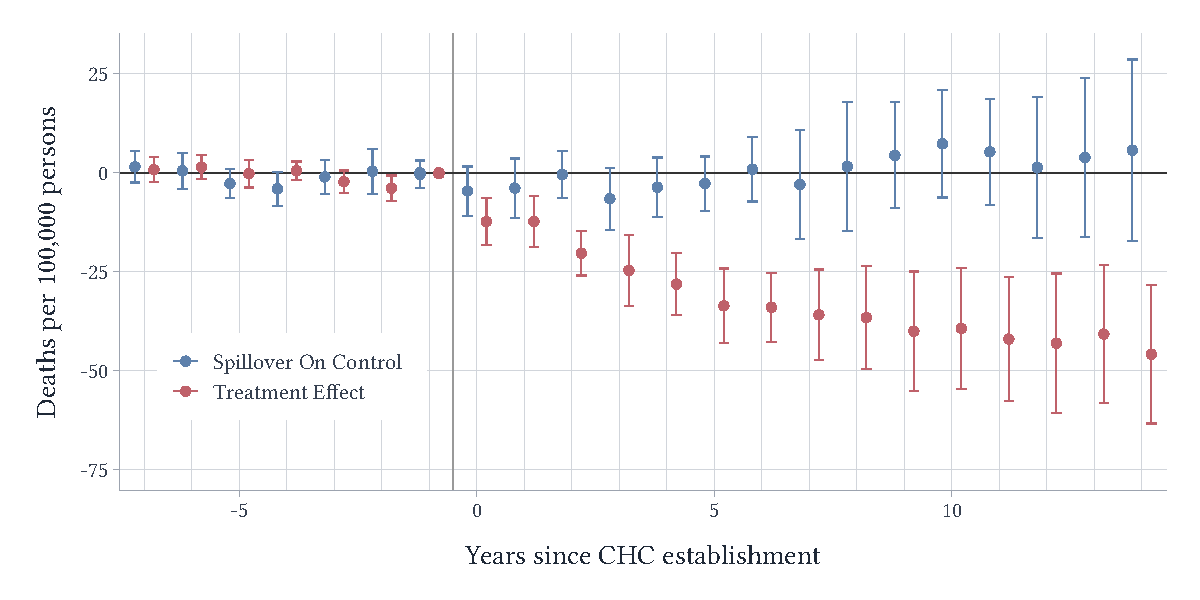
\includegraphics[width=\textwidth]{figures/spatial-spillovers/chc/chc-es_combined.pdf}
  }
  {\footnotesize
    \textit{Notes:} This figure plots event study estimates for the total effect and the spillover effect on control units within 25 miles of treatment at different periods relative to establishment year. The estimates are generated using the `did2s' package \citep{did2s}. 
  }
\end{figure}

There are theoretical reasons to think spillovers may or may not exist in this context. On the one hand, individuals outside the county can potentially travel to the community health centers to receive care. This would create a negative spillover effect on mortality rates in nearby counties which would bias their estimates towards zero. On the other hand, \citet{Bailey_Goodman_Bacon_2015} document evidence that their estimated effects are not due to emergencies but rather primary care services. In this case, it is less likely low-income individuals would travel very far to receive primary care, and hence the spillover effects are potentially near zero. My methodology can provide an answer to the question of how far do individuals travel for low-/no-cost primary care.

As in the method detailed above, I use an indicator for being within 25 miles of a treated county as the spillover variable. The results are presented in Figure \ref{fig:chc_es_spill}. The confidence intervals labeled with circles represent point estimates for the average spillover effect on control units within 25 miles. No spillover effect is estimated to be significantly different from zero which suggests that the effects of community health centers are very local. Since there are near zero spillover effects, the total effect estimates marked in Figure \ref{fig:chc_es_spill} as diamonds maintain the same shape as the author's original estimates with estimates between 15-30 fewer deaths per 100,000 persons. 

The spillover effects results provide evidence that low-income individuals will not travel far to receive primary care. Practically, this suggests that community health centers should be targeted to be as accessible as possible for poor individuals as they are unable to travel far to access the services. 

% ------------------------------------------------------------------------------
\section{Discussion}
\label{sec:conclusion}
% ------------------------------------------------------------------------------

This paper has considered the common environment where treatment is assigned to groups of units while the effects of treatment spread across these borders. I model this phenomenon using a potential outcomes framework and show why standard difference-in-differences estimation does not identify treatment effects of interest. Next, I discuss identification of two well-defined treatment effects. First, the average local effect of a single unit changing their treatment status is hard to identify without imposing assumptions on the spillover mapping. The second effect, the post-hoc average total effect on the treated is more simply identified under the assumption that spillovers are local. Effects can be identified by using far-away control units, but the practical usefullness of this result depends on whether far-away control units satisfy the parallel counterfactual trends. Last, I show how to extend the estimation strategy proposed in the paper to settings with staggered treatment-timing, a recent concern in the literature. 

I use a set of empirical examples to show that in settings with spatial spillovers, estimates can change significantly. In particular, place-based interventions change the nature of agglomeration in the local and surrounding area--that is cause spillovers--local effects of these policies can be misestimated without controlling for general equilibrium effects. I also show the importance of considering spillovers in weighing the pros and cons of various identification strategies. Identification strategies based on geographic continuity of unobservables can magnify the bias from spillovers as they restrict the comparison group to observations experiencing the largest spillover effects.




\chapter{Difference-in-Differences with Geocoded Microdata}\label{chapter:geocoded}


% Paper ------------------------------------------------------------------------

% ------------------------------------------------------------------------------
\section{Introduction}
% ------------------------------------------------------------------------------

The rise of geocoded microdata has allowed researchers to begin answering questions about the effects of spatially-targeted treatments at a very granular level. How do local pollutants affect child health?\footnote{See, e.g., \citet{Currie_Davis_Greenstone_Walker_2015} and \citet{Marcus_2021}.} Does living within walking distance to a new bus stop improve labor market outcomes?\footnote{See, e.g., \citet{gibbons2005valuing} and \citet{billings2011estimating}.} How far do neighborhood shocks, such as foreclosures or new construction spread?\footnote{See, e.g., \citet{Asquith_Mast_Reed_2021,cui2015foreclosure,Gerardi_Rosenblatt_Willen_Yao_2015} and \citet{Campbell_Giglio_Pathak_2011}.} A standard method of evaluating the effects of the treatment is to compare changes in outcomes for units that are close to treatment to those slightly further away -- what I label the `ring method' as illustrated in \autoref{fig:example-id}. This paper formalizes the assumptions required for identification in the ring method, highlighting potential pitfalls of the currently-used estimator, and proposes an improved estimator. 

First, I formalize the necessary assumptions for unbiased estimates of the average treatment effect on the affected units.\footnote{This generalizes the treatment effect on the treated in the case where treatment is not assigned to specific units.} The first assumption is the well understood parallel trends assumption for the treated and control units. This requires that the \textit{average} change in (counterfactual) untreated outcomes in the treated ring is equal to the \textit{average} change in the control ring. The rings method is typically motivated by the fact that since the treated and control units are all very close in physical location, e.g. having access to the same labor market and consumptive amenities, shocks over time should be common across units in the neighborhood.\footnote{For example, \citet{Asquith_Mast_Reed_2021} write "The idea is that within a small area, developers have few sites that are available and properly zoned, leading to hyper-local variation in the location of new construction that is not related to future price changes."} 

Instead of \textit{fully} leveraging the common neighborhood trends assumption that motivates the ring method, researchers rely on a second assumption which requires correct identification of how far treatment effects are experienced (the inner ring). This is a very strict assumption that when not satisfied, causes biased estimates of the treatment effect. If the treated ring is too narrow, then units in the control ring experience effects of treatment and the change among `control' units would no longer identify the counterfactual trend. On the other hand, if the treated ring is too wide, then the zero treatment effect of some unaffected units are averaged into the change among `treated' units. Therefore, results will be attenuated towards zero.

% Figure: Example ID -----------------------------------------------------------

\begin{figure}[tb]
  \caption{Rings Method}
  \label{fig:example-id}

  \begin{adjustbox}{width = 0.4\textwidth, center}
      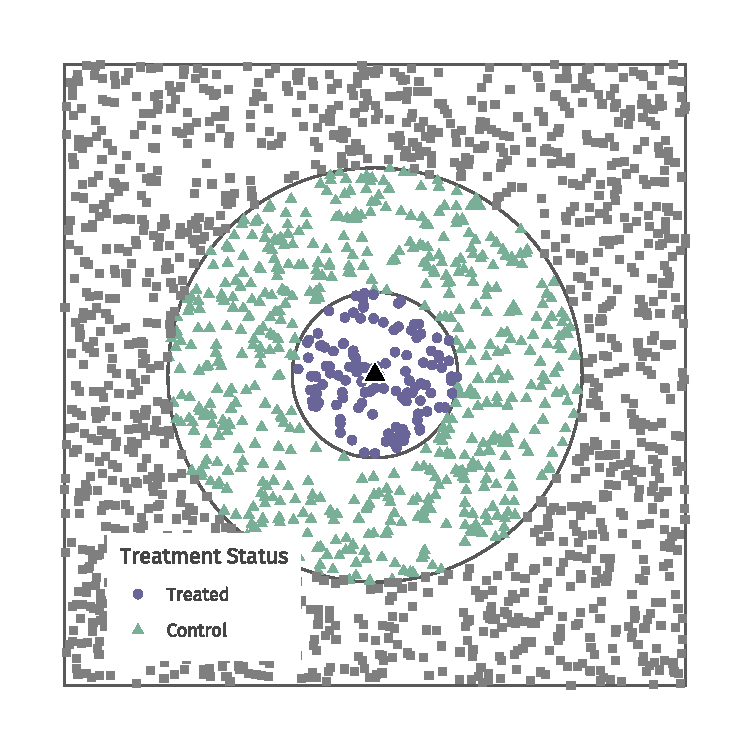
\includegraphics[width=\textwidth]{figures/geocoded/example_id.pdf}
  \end{adjustbox}

  \note{This figure illustrates the ring method. The center triangle represents the location of treatment, e.g. a foreclosed home. Units within the inner circle, marked by dots, are considered `treated'; units between the inner and outer circles, marked in triangles, are considered control units; and then the remaining units are removed from the sample. The ring estimate compares average changes in outcomes between the inner `treated' ring and the outer `control' ring.}
\end{figure}

I propose an alternative estimator that fully leverages the `common neighborhood trends' assumption using a nonparametric partitioning-based least square estimator \citep{cattaneo2019binscatter,Cattaneo_Farrell_Feng_2019}. My proposed methodology estimates the treatment effect curve as a function of distance by using many rings rather than trying to estimate the average treatment effect with one inner ring. This method requires that treatment effects become zero somewhere between the distance of 0 and the outer ring \textit{without} the need to specify the \textit{exact} distance at which it does. To do this, the estimator leverages the stronger `common neighborhood trends' assumption that the counterfactual trend is constant across distance. This new assumption is more strict in that the standard method only requires that parallel trends holds \textit{on average} in each ring. However, researchers typically motivate the identification strategy by saying within a small distance from treatment that units are subject to a common set of shocks which implies the more strict assumption. While this assumption is not directly testable, my proposed estimator creates a set of point estimates of treatment effects that can be used to visually inspect the plausability of the assumption. If after some distance, treatment effects become centered at zero, this suggests that common trends hold, akin to the pre-trends test in event study regressions.

The nonparametric estimator provides many benefits. First, the estimator allows the researcher to get a more complete picture of how the intervention affects units at various distances rather than estimating an ``overall effect''. For example, a new bus-stop potentially creates net costs to immediate neighbors while providing net benefits for homes slightly further away. Estimation of the treatment effect curve can illustrate these different effects that a single ring may average out to near-zero effects. Additionally, the proposed nonparametric estimator selects the rings in a \textit{completely data-driven and optimal manner} removing incentives for specification searching or `pre-testing' the data to determine the `correct' rings \citep{mccloskey2020critical,andrews2019identification}.

This paper contributes to the literature in many ways. First, I contribute to a literature that discuss identification using the rings method. \citet{Sullivan_2017} and \citet{Gerardi_Rosenblatt_Willen_Yao_2015} discuss the identification assumption of identifying the maximum treatment distance. My paper formalizes all the necessary assumptions for identification in the ring method. Other researchers have recognized that estimating a single average treatment effect is less informative than a treatment effect curve, instead using multiple rings to estimate treatment effects at different distances (e.g. \citet{Alexander_Currie_Schnell_2019,Casey_Schiman_Wachala_2018,di2004police}). However, this approach selects multiple rings in an ad-hoc manner, requires treatment effects to become zero after the outer-most treatment ring, and is prone to problems of specification searching. The current study's proposed estimator selects the number and location of rings in a data-driven way and does not require correct specification of where treatment effects become zero.

\citet{diamond2019wants} propose an alternative nonparametric estimator aimed at estimating a treatment effect surface. Similar to this paper, they leverage the "common local trends" assumption to estimate a \textit{two-dimensional} treatment effect curve. Their procedure allows ``location'' fixed effects to differ along two-dimensions, latitude and longitude (e.g. the mean home price is higher in the north-west than the south-east) which in cross-sectional data can absorb more variation in the data yielding smaller standard errors than my method, though both are consistent. In the case of panel data, this does not matter since first-differencing remove this systematic variation. To produce noise estimates/standard errors, their method requires integrating over the 2D curve for arbitrarily chosen rings. In cases where researchers chose these aggregation ranges based on the results of the estimation procedure, standard inference tools are not valid even when bootstrapping the standard errors \citep{leeb2005model}. As discussed above, my proposed estimator provides valid inference after selection of aggregation regions and choses these aggregation regions in a data-driven manner.

This paper also contributes to a small literature on difference-in-differences estimators from a spatial lens \citep{Butts_2021,Clarke_2017,Berg_Streitz_2019,verbitsky2012causal,Delgado_Florax_2015}. These papers address instances where treatment is well defined by administrative boundaries but spillovers cause problems of defining who is `treated' and at what level of exposure. This paper contributes to this literature by considering the setting where treatment occurs at a point in space. \citet{Butts_2021} and \citet{Clarke_2017} both recommend a method of using many rings to estimate a treatment effect curve, but are not able to provide a data-driven way to select the rings. Since this paper focuses on local shocks where constant parallel trends are plausible, I am able to provide a data-driven approach to choosing rings. 

% ------------------------------------------------------------------------------
\section{Example of Problem}\label{sec:example}
% ------------------------------------------------------------------------------

% Figure: Example problem ------------------------------------------------------

\begin{figure}[tb]
  \caption{Example of Problems with Ad-Hoc Ring Selection}
  \label{fig:problems}
  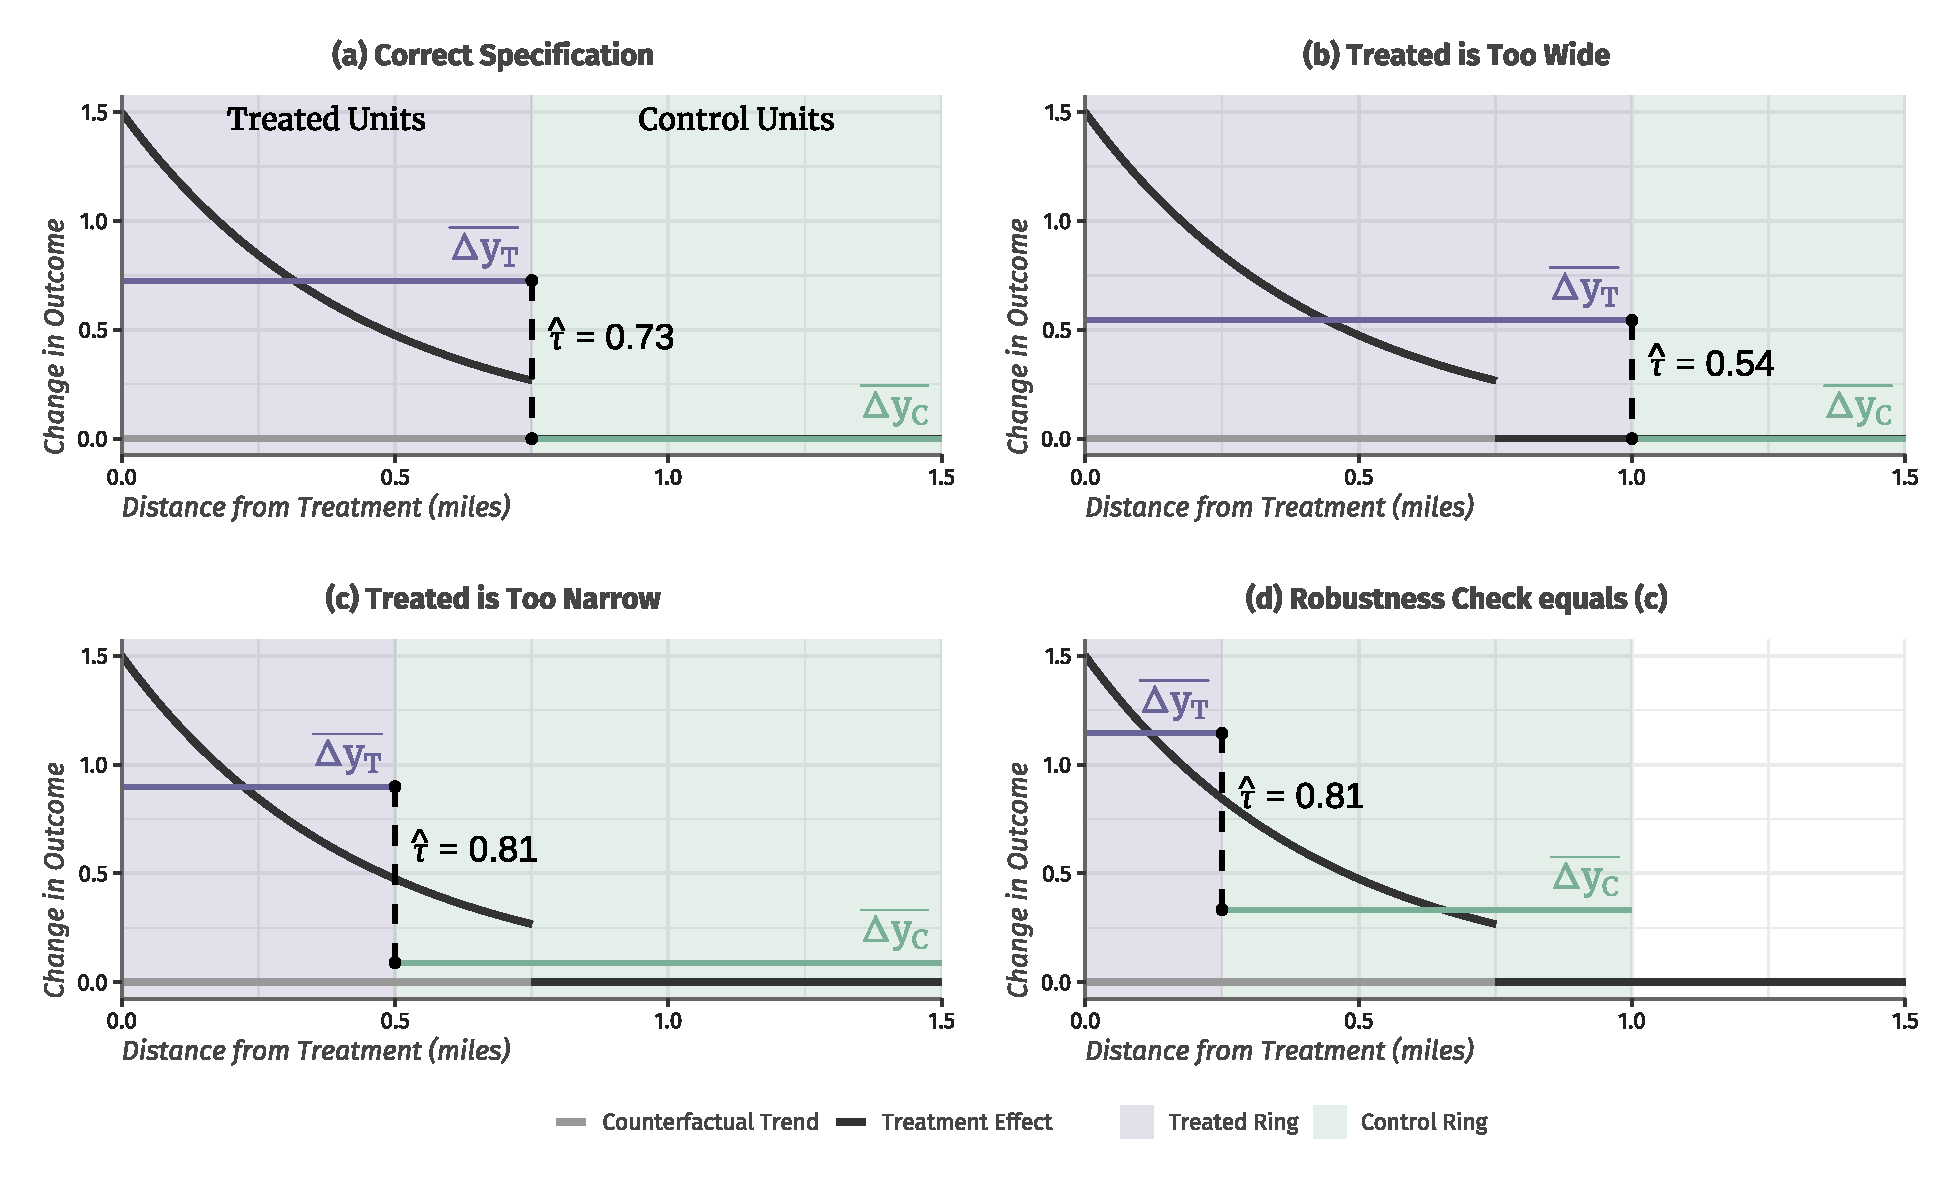
\includegraphics[width=\textwidth]{figures/geocoded/example.pdf}

  \note{This figure shows an example of the difficulties in estimation of treatment effects via the ring method.}
\end{figure}

To illustrate the methodological difficulties in this method, suppose that an overgrown empty lot in a high-poverty neighborhood is cleaned up by the city and the outcome of interest is home prices. The researcher observes a panel of home sales before and after the lot is cleaned. \autoref{fig:problems} shows a plot of simulated data from this example. The black line is treatment effect at different distances from the empty lot and the grey line is the underlying (\textit{constant}) counterfactual change in home prices, normalized to 0. Panel (a) of \autoref{fig:problems} shows the best-case scenario where the treated ring is correctly specified. The two horizontal lines show the average change in outcome in the treated ring and the control ring and our treatment effect estimate, $\hat{\tau}$, is the difference between these two averages. However, this singular number masks over a large amount of treatment effect heterogeneity with units experiencing treatment effects as little as half and as large as double the magnitude that of $\hat{\tau}$. Later in this paper, I recommend nonparametrically estimating the treatment effect curve as a function of distance rather than using average effect. 

However, the researcher does not typically know the distance at which treatment effects stop. Panel (b) shows when the `treatment' ring is too wide. In this case, some of the units in the treatment ring receive no effect from treatment and therefore makes the average treament effect among units in the treatment ring smaller. Panel (c) of \autoref{fig:problems} shows the opposite case, where the treated ring is too narrow. In this case, there are some units in the `control' ring that experience treatment effects and the coutnerfactual trend estimate is biased upward. The treatment effect estimate grows since the new `treated' group is closer and hence experiences larger treatment effects. Panel (d) of \autoref{fig:problems} shows an example of why using different rings as a `robustness check' is a problematic practice. Using Panel (d) as a robustness check for the researchers' original specification of Panel (c), a researcher would be quite confident in their results even though the estimate is too large in both cases.

From these three examples, it's clear that the estimation strategy requires researchers to know the exact distance at which treatment effects become zero. Since this is a very demanding assumption, I propose an improved estimator in \autoref{sec:lspartition} that relaxes this assumption by leveraging the constant common trends assumption. 




% ------------------------------------------------------------------------------
\section{Theory}
% ------------------------------------------------------------------------------

Now, I develop econometric theory to formalize the intuition developed in the previous section. A researcher observes panel data of a random sample of units $i$ at times $t = 0, 1$ located in space at point $\theta_i = (x_i, y_i)$. Treatment occurs at a location $\bar{\theta} = (\bar{x}, \bar{y})$ between periods. Therefore, units differ in their distance to treatment, defined by $\dist_i \equiv d(\theta_i, \bar{\theta})$ for some distance metric $d$ (e.g. Euclidean distance) with a distribution function $F$. Outcomes are given by 
\begin{equation}
    Y_{it} = \mu_i + \tau_i \one_{t = 1} + \lambda_i \one_{t=1} +u_{it},    
\end{equation}
where $\mu_i$ is unit-specific time-invariant factors, $\lambda_i$ is the change in outcomes due to non-treatment shocks in period 1, $\tau_i$ is unit $i$'s treatment effect. Both $\lambda$ and $\tau$ can be split into a systematic function of distance $z(\dist_i)$ and an idiosyncratic term $\tilde{z}_i \equiv z_i - z(\dist_i)$ with $z$ being $\tau$ and $\lambda$. $\tau(d)$ is the average effect of treatment at a given distance and $\lambda(d)$ summarizes how covariates and shocks change over distance.

Therefore, we could rewrite our model as 
\begin{equation}\label{eq:model}
    Y_{it} = \mu_i + \tau(\dist_i) \one_{t = 1} + \lambda(\dist_i) \one_{t=1} + \varepsilon_{it},   
\end{equation}
where $\varepsilon = u_{it} + \tilde{\tau}_i + \tilde{\lambda}_i$ which is uncorrelated with distance to treatment. Researchers are trying to identify the average treatment effect on units experiencing treatment effects, i.e. $\bar{\tau} = \expec{\tau_i}{\tau(\dist_i) > 0}$.

\begin{assumption}[Random Sampling]
    The observed data consists of $\{ Y_{i1}, Y_{i0}, \dist_{i}\}$ which is independent and identically distributed.
\end{assumption}

Taking first-differences of our model, we have $\Delta Y_{it} = \tau(\dist_i) + \lambda(\dist_i) + \Delta \varepsilon_{it}$. It is clear that $\tau(\dist_i)$ and $\lambda(\dist_i)$ are not seperately identified unless additional assumptions are imposed. The central identifying assumption that researchers claim when using the ring method is that counterfactual trends likely evolve smoothly over distance, so that $\lambda(\dist_i)$ is approximately constant within a small distance from treatment. This is formalized in the context of our outcome model by the following assumption. 

\begin{assumption}[Local Parallel Trends]\label{assum:parallel}
    For a distance $\bar{d}$, we say that `local parallel trends' hold if for all positive $d, d' \leq \bar{d}$, then $\lambda(d) = \lambda(d')$.
\end{assumption}

This assumption requires that, in the absence of treatment, outcomes would evolve the same at every distance from treatment within a certain maximum distance, $\bar{d}$. To clarify the assumption, it is helpful to think of ways that it can fail. First, if treatment location is targeted based on trends \textit{within a small-area/neighborhood}, then trends would not be constant within the control ring. Second, if units sort either towards or away from treatment in a way that is systematically correlated with the outcome variable, then the compositional change can cause a violation in trends over time. Note that \nameref{assum:parallel} implies the standard assumption that parallel trends holds \textit{on average} between the treated and control rings:

\begin{assumption}[Average Parallel Trends]\label{assum:parallel_weak}
    For a pair of distances $d_t$ and $d_c$, we say that `average parallel trends' hold if $\expec{\lambda_d}{0 \leq d \leq d_t} = \expec{\lambda_d}{d_t < d \leq d_c}$.
\end{assumption}

If \nameref{assum:parallel} holds for some $d_c$, then our first-difference equation can be simplified to $\Delta Y_{it} = \tau(\dist_i) + \lambda + \Delta \varepsilon_{it}$ where $\lambda$ is some constant for units in the subsample $\mathcal{D} \equiv \{i \ : \ \dist_i \leq d_c \} $. Therefore, the treatment effect curve $\tau(\dist_i)$ is identifiable up to a constant under Assumption \ref{assum:parallel}. To identify $\tau(\dist_i)$ seperately from the constant, researchers will often claim that treatment effects stop occuring before some distance $d_t < d_c$. This is formalized in  the following assumption. 

\begin{assumption}[Correct $d_t$]\label{assum:dt}
    A distance $d_t$ satisfies this assumption if (i) for all $d \leq d_t$, $\tau(d) > 0$ and for all $d > d_t$, $\tau(d) = 0$ and (ii) $F(d_c) - F(d_t) > 0$.
\end{assumption}

With this assumption, the first difference equation simplifies to $\Delta Y_{it} = \lambda + \Delta \varepsilon_{it}$ for units with $d_t < \dist_i < d_c$. These units therefore identify $\lambda$. The `ring method' is the following procedure. Researchers select a pair of distances $d_t < d_c$ which define the ``treated'' and ``control'' groups. These groups are defined by $\mathcal{D}_t \equiv \{ i : 0 \leq \dist_i \leq d_t \}$ and $\mathcal{D}_c \equiv \{ i : d_t < \dist_i \leq d_c \}$. On the subsample of observations defined by $\mathcal{D} \equiv \mathcal{D}_t \cup \mathcal{D}_c$, they estimate the following regression:

\begin{equation}\label{eq:ring_method}
    \Delta Y_{it} = \beta_0 + \beta_1 \one_{i \in \mathcal{D}_t} + u_{it}.
\end{equation}

From standard results for regressions involving only indicators, difference-in-differences estimator is $\hat{\beta}_1$ with the following expectation:
\[
    \expec{\hat{\beta}_1} = \expec{\Delta Y_{it}}{\mathcal{D}_t} - \expec{\Delta Y_{it}}{\mathcal{D}_c}.
\]
This estimate is decomposed in the following proposition.\footnote{A similar derivation of part (i) is found in \citet{Sullivan_2017} but does not include difference in parallel trends.}

\begin{proposition}[Decomposition of Ring Estimate]\label{prop:ring_decomp}  
    Given that units follow model (\ref{eq:model}),
    \begin{enumerate}
        \item[(i)] The estimate of $\beta_1$ in (\ref{eq:ring_method}) has the following expectation:
        \begin{align*}
            \expec{\hat{\beta}_1} &= \expec{\Delta Y_{it}}{\mathcal{D}_t} - \expec{\Delta Y_{it}}{\mathcal{D}_c} \\
            &=  \underbrace{\expec{\tau(\dist)}{\mathcal{D}_t} - \expec{\tau(\dist)}{\mathcal{D}_c} }_{\text{Difference in Treatment Effect}} + \underbrace{\expec{\lambda(\dist)}{\mathcal{D}_t} - \expec{\lambda(\dist)}{\mathcal{D}_c} }_{\text{Difference in Trends}}.
        \end{align*}
        
        \item[(ii)] If $d_c$ satisfies \nameref{assum:parallel} or, more weakly, if $d_t$ and $d_c$ satisfy \nameref{assum:parallel_weak}, then
        \[ 
            \expec{\hat{\beta}_1} = 
            \underbrace{\expec{\tau(\dist)}{\mathcal{D}_t} - \expec{\tau(\dist)}{\mathcal{D}_c} }_{\text{Difference in Treatment Effect}}.
        \] 
    
        \item[(iii)] If $d_c$ satisfies \nameref{assum:parallel} and $d_t$ satisfies Assumption \ref{assum:dt}, then
        \[ 
            \expec{\hat{\beta}_1} = \bar{\tau}.
        \]
    \end{enumerate}
\end{proposition}

Part (i) of this proposition shows that the estimate is the sum of two differences. The first difference is the difference in average treatment effect among units in the treated ring and units in the control ring. The second difference is the difference in counterfactual trends between the treated and control rings. This presents two possible problems. If some units in the control group experience effects from treatment, the average of these effects will be subtracted from the estimate. Second, since treatment can be targeted, the treated ring could be on a different trend than units further away and hence control units do not serve as a good counterfactual for treated units.

Part (ii) says that if $d_c$ satisfies \nameref{assum:parallel}, then the difference in trends from part (i) is equal to 0. As discussed above, the decomposition in part (ii) of Proposition \ref{prop:ring_decomp} is not necessarily unbiased estimate for $\bar{\tau}$. First, if $d_t$ is \textit{too wide}, then $\mathcal{D}_t$ contain units that are not affected by treatment. In this case, $\hat{\beta}_1$ will be biased towards zero from the inclusion of unaffected units from $d_t$ being too wide. Second, if $d_t$ is \textit{too narrow} then the $\mathcal{D}_c$ will contain units that experience treatment effects. It is not clear in this case, though, whether $\hat{\beta}_1$ will grow or shrink without knowledge of the $\tau(\dist)$ curve, but typically $\hat{\beta}_1$ will not be an unbiased estimate for $\bar{\tau}$. See the previous section for an example.  

Part (iii) of Proposition \ref{prop:ring_decomp} shows that if $d_t$ is correctly specified as the maximum distance that receives treatment effect, then $\hat{\beta}_1$ will be an unbiased estimate for the average treatment effect among the units affected by treatment. However, Assumption \ref{assum:dt} is a very demanding assumption and unlikely to be known by the researcher unless there are \textit{a priori} theory dictating $d_t$.\footnote{As an example, \citet{Currie_Davis_Greenstone_Walker_2015} uses results from scientific research on the maximum spread of local pollutants and \citet{Marcus_2021} use the plume length of petroleum smoke.} The following section will improve estimation by allowing consistent nonparametric estimation of the entire $\tau(\dist)$ function. An estimate of $\tau(\dist)$ can then be numerically integrated to for an estimate of $\bar{\tau}$.



% ------------------------------------------------------------------------------
\section{Nonparametric Estimation of the Treatment Effect Curve}\label{sec:lspartition}
% ------------------------------------------------------------------------------

In this section, I propose an estimation strategy that nonparametrically identifies the treatment effect curve $\tau(\dist_i)$ using partitioning-based least squares estimation and inference methods developed in \citet{cattaneo2019binscatter, Cattaneo_Farrell_Feng_2019}. Partition-based estimators seperate the support of a covariate, $\dist_i$, into a set of quantile-spaced intervals (e.g. 0-25th percentiles of $\dist_i$, 25-50th, 50-75th, and 75-100th). Then the conditional $\expec{Y_i}{\dist_i}$ is estimated seperately within each interval as a $k$-degree polynomial of the covariate $\dist_i$.

For a given outer-ring distance, $d_c$, our sample is given by $\mathcal{D} = \{ i : \dist_i \leq d_c \}$. We will split the sample into $L$ intervals based on quantiles of the distance variable. For a given $j \in \{1, \dots, L\}$, I denote the $j^{th}$ interval as $\mathcal{D}_j \equiv\{ i : F_n^{-1}(\frac{j-1}{L}) \leq \dist_i < F_n^{-1}(\frac{j}{L}) \}$ where $F_n$ is the empirical distribution of $\dist$. Let $\{ \mathcal{D}_1, \dots, \mathcal{D}_L \}$ be the collection of the $L$ intervals. This paper will use a $0$-degree polynomial for each interval, predicting $\Delta Y_{it}$ with a constant within each interval.\footnote{Approximation can be made arbitrarily close to the true conditional expectation function by \textit{either} increasing the number of intervals \textit{or} by increasing the polynomial order to infinity, so setting $k = 0$ does not impose any asymptotic cost.} These averages are defined as 
\[
    \overline{\Delta Y}_j \equiv \frac{1}{n_j} \sum_{i \in \mathcal{D}_j} \Delta Y_{it},
\]
where the number of units in bin $\mathcal{D}_j$ is $n_j \approx n/L$. Our estimator for $\expec{\Delta Y_{it}}{\dist_i}$ is then given by
\[
    \widehat{\Delta Y_{it}} = \sum_{j = 1}^{L} \one_{i \in \mathcal{D}_j} \overline{\Delta Y}_j
\]
As the number of intervals approach infinity, this estimate will approach $\expec{\Delta Y_{it}}{\dist = d}$ uniformly. Under \nameref{assum:parallel}, $\expec{\Delta Y_{it}}{\dist = d} \equiv \expec{\tau(\dist)}{\dist = d} + \lambda$. To remove $\lambda$, we require a less-strict version of assumption \ref{assum:dt}.

\begin{assumption}[$d_t$ is within $d_c$]\label{assum:dt_weak}
    A distance $d_c$ satisfies this assumption if there exists a distance $d_t$ with $0 < d_t < d_c$ such that (i) Assumption \ref{assum:dt} holds and (ii) $F(d_c) - F(d_t) > 0$.
\end{assumption}

If a distance $d_c$ satisfies \nameref{assum:parallel} and (\ref{assum:dt_weak}), the mean within the last ring $\mathcal{D}_k$ will estimate $\lambda$ as the number of bins $L \to \infty$. The reason for this is simple, as $L \to \infty$, the last bin will have a left end-point $> d_t$ and therefore $\tau(\dist) = 0$ in $\mathcal{D}_L$. Under local parallel trends, the last ring will therefore estimate $\lambda$. Therefore, estimates of $\tau(\dist_i)$ can be formed for each interval as $\hat{\tau}_j \equiv \overline{\Delta Y}_j - \overline{\Delta Y}_L$. These $\hat{\tau}_j$ can be plotted over their intervals to provide a graphical estimate of the treatment effect curve (see below for an example).

\begin{proposition}[Consistency of Nonparametric Estimator]\label{prop:np_identification}  
    Given that units follow model (\ref{eq:model}) and $d_c$ satisfies \nameref{assum:parallel} and assumption (\ref{assum:dt_weak}), as $n$ and $L \to \infty$ 

    \begin{align*}
        \hat{\tau} &\equiv \sum_{i=1}^L \hat{\tau}_j 1_{i \in \mathcal{D}_j} \to^{unif} \tau(\dist)
    \end{align*}

    under regularity conditions given by Assumption (1) of \citet{Cattaneo_Farrell_Feng_2019}, $L \log(L)/n \to 0$ and $nL^{-5} \to 0$.\footnote{See \autoref{sec:geocoded-proofs} for the proof.}
\end{proposition}

As discussed in \autoref{sec:example}, specifying $d_t$ correctly is important to identify the average treatment effect among the affected in the parametric estimator. The nonparametric estimator only requires that treatment effects become zero before $d_c$, i.e. that such a $d_t$ exists. However, the estimator comes at a cost, namely it would no longer identify the treatment effect curve under the milder \nameref{assum:parallel_weak} assumption. Therefore, a researcher should justify explicity the assumption that, within the $d_c$ ring, every unit is subject to the same trend. This is most likely to be satisfied on a very local level and not very plausible in the case of larger units, e.g. counties.

The nonparametric approach allows estimation of the treatment effect curve which allows researcher to understand differences in treatment effect across distance whereas the indicator approach, \textit{at best}, can only estimate an \textit{average} effect among units experiencing effects. For example, typically one would assume treatment effects shrink over distance and evidence of this from the nonparametric approach can strengthen a causal claim. In some cases, such as a negative hyper-local shock and a postivie local shock (e.g. a local bus-stop), the treatment effect can even change sign across distances. In this case, the average effect could be near zero even though there are significant effects occuring. 

Plotting estimates $\hat{\tau}_j$ can provide visual evidence for the underlying \nameref{assum:parallel} assumption. Typically, treatment effect will stop being experienced far enough away from $d_c$ that some estimates of $\hat{\tau}_j$ with $j$ `close to' $L$ will provide informal tests for parallel trends holding. \autoref{fig:lr} provide an example where plotting of $\hat{\tau}_j$ provide strong evidence in support of local parallel trends as it appears that after some distance, average effects are consistetly centered around zero. This is not a formal test as it could be the case that the true treatment effect curve, $\tau(\dist)$ is perfectly cancelling out with the counterfactual trends curve $\lambda(\dist)$ producing near zero estimates, but this is a knive's edge case. 

The above proposition shows that the series estimator will consistenly estimate the treatment effect curve, $\tau(\dist)$ as the number of bins $L$ and the number of observations $n$ both go to infinity. In finite-samples though, we will have a fixed $L$ and hence a fixed set of treatment effect estimates $\{ \tau_1, \dots, \tau_{L}\}$ with $\tau_L \equiv 0$ by definition. The estimates $\hat{\tau}_j$ are approximately equal to $\expec{\tau(\dist)}{\dist \in \mathcal{D}_j}$ or the average treatment effect within the interval $\mathcal{D}_j$.

The choice of $L$ in finite samples is not entirely clear. \citet{cattaneo2019binscatter} derive the optimal choice of $L$ which is a completely data-driven choice. The optimal $L$ is driven by two competing terms in the mean-squared error formula. On the one hand, as $L$ increases, the conditional expectation function is allowed to vary more across values of $\dist$ and hence bias of the estimator decreases. However, larger values of $L$ increase the variance of the estimator. Balancing this trade-off depends on the shape and curvature of $\tau(\dist)$ which is estimated by the data. The resulting choice of $L^*$ determines the number of bins and the rings are determined by quantiles of the data. Since the rings are themselves estimated, \citet{cattaneo2019binscatter} provide inference that is valid after the `first-stage' estimation of quantiles. 

This data-driven choice allows for estimation in a principled and objective way that lets the data `speak for itself'. Further, this method removes incentives from `pre-testing' the choice of rings to find a significant result since the estimates are determined completely by the data \footnote{See, for example, discussions in \citet{andrews2019identification} and \citet{mccloskey2020critical} about researcher degrees of freedom.} 

For a given $L^*$, \citet{cattaneo2019binscatter} show the large-sample asymptotics of the estimates $\overline{\Delta Y}_j$ and provide robust standard errors for the conditional means that account for the additional randomness due to quantile estimation. Since our estimator is a difference in means, standard errors on our estimate $\hat{\tau}_j$ are given by $\sqrt{\sigma^2_j + \sigma^2_L}$, where $\sigma_j$ is the standard error recommended by \citet{cattaneo2019binscatter}. These standard errors are produced by the Stata/R package \texttt{binsreg}. Inference can be done by using the estimated t-stat with the standard normal distribution. There may be concerned that the standard errors need to adjust for spatial correlation. However, this is not the case under assumption (\ref{assum:parallel}) as this implies the error term is uncorrelated with distance.

\begin{remark}[Overall Average Treatment Effect]
A researcher may be tempted to `pool' together the significant rings to estimate an overall average treatment effect among the affected. Since the estimates are quantiles in the data, a simple average of the significant $\hat{\tau}_j$'s can produce a back of the envelope treatment effect. However, infernece on this estimand is not possible, since, in repeated sampling the number of significant $\hat{\tau}_j$ can change and this additional source of `model selection' makes inference a very difficult problem \citep{leeb2005model}. A potential solution would be to use cross-validation where half the data would determine the `inner ring' and then the second half of the data would estimate the overall average treatment effect, though potentially requiring a large sample size.
\end{remark}

\begin{remark}[Covariates]
A researcher may often be interested The partitioning based series-estimator can allow for covariates to be included in the model with valid inference, so the estimation can easily be done with the Stata/R package \texttt{binsreg}. However, including covariates changes the necessary common trends assumption to have to hold conditional on the vector of covariates $X$ (See \citet{santanna2020doubly} for modern discussion of conditonal parallel trends). In this paper, this estimation strategy would require neighborhood shocks to be common across values of $X_i$, i.e. shocks are experienced equally regardless of characteristics $X$.
\end{remark}



% ------------------------------------------------------------------------------
\section{Application to Neighborhood Effects of Crime Risk}
% ------------------------------------------------------------------------------

To highlight the advantages of my proposed estimator, I revisit the analysis of \citet{Linden_Rockoff_2008}. This paper analyzes the effect of a sex offender moving to a neighborhood on home prices. This paper uses the ring method with treated homes being defined as being within $1/10^{th}$ of the sex offender's home and the control units being between $1/10^{th}$ and $1/3^{rd}$ of a mile from the home. The authors make a case for the ring method by arguing that \textit{within a neighborhood}, \nameref{assum:parallel} holds since they are looking in such a narrow area and purchasing a home is difficult to be precisely located with concurrent hyper-local shocks. This application uses cross-sectional data which similar identification and estimation results are presented in the Appendix.


\begin{figure}[htb!]
    \caption{Price Gradient of Distance from Offender}\label{fig:lr_nonparametric}

    \begin{subfigure}{0.33\textwidth}
        \caption{Bandwidth of 0.025}
    \end{subfigure}
    \begin{subfigure}{0.33\textwidth}
        \caption{Bandwidth of 0.075}
    \end{subfigure}
    \begin{subfigure}{0.33\textwidth}
        \caption{Bandwidth of 0.125}
    \end{subfigure}
    
    \vspace{-3mm}
    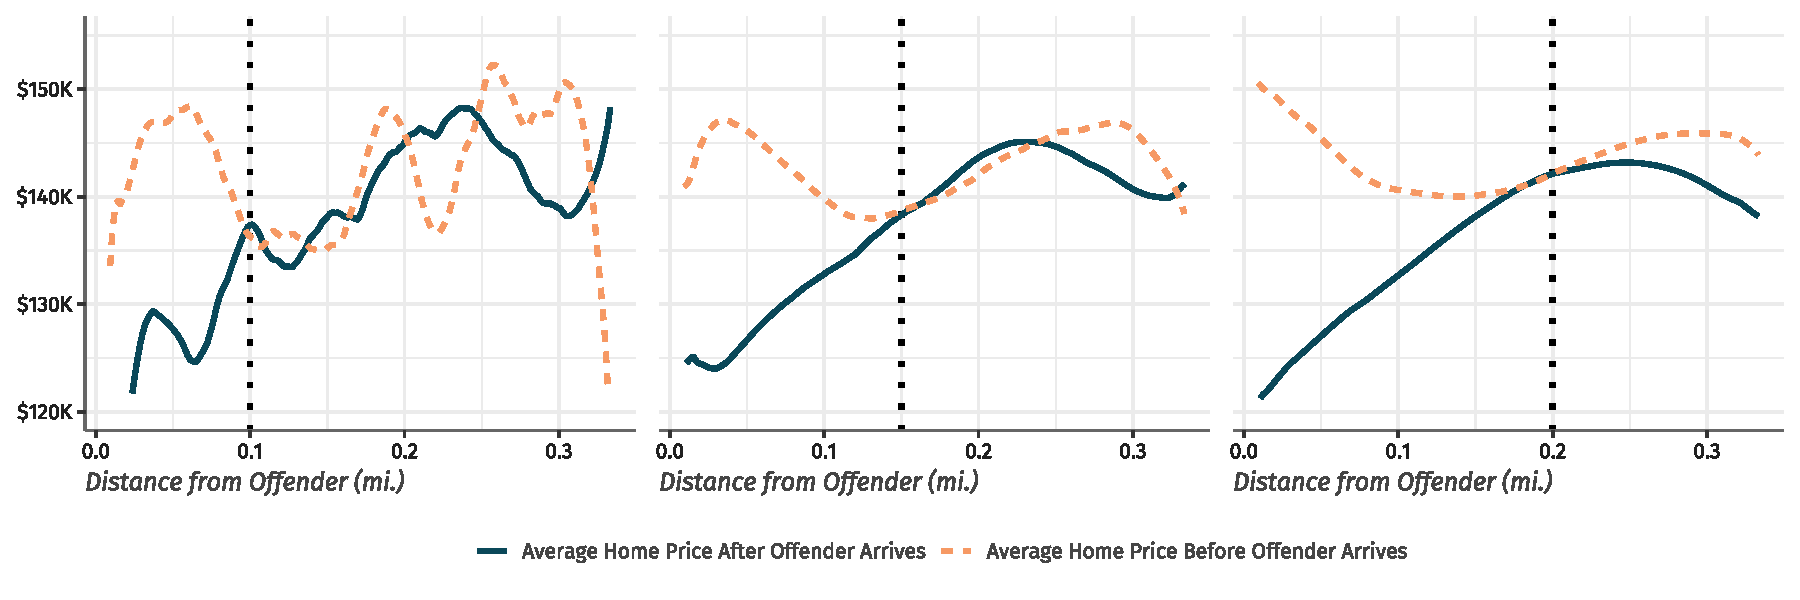
\includegraphics[width=\textwidth]{figures/geocoded/linden_rockoff_nonparametric.pdf}
    

    \note{This figure plots estimates of home prices in the year before and the year after the arrival of a sex offender estimated using a Local Polynomial Kernel Density estimation with an Epanechnikov kernel. Panel (b) recreates Figure 2 from \citet{Linden_Rockoff_2008} and the other panels change the bandwidth.}
\end{figure}

As for the choice of the treatment ring, there is little \textit{a priori} reasons to know how far the effects of sex offender arrival will extend in the neighborhood. The authors provide graphical evidence of nonparametric estimates of the conditional mean home price at different distances in the year before and the year after the arrival of a sex offender. The published plot can be seen in Panel (b) of \autoref{fig:lr_nonparametric}. They `eyeball' the point at which the two estimates are approximately equal to decide how far treatment effects extend. However, this approach is less precise than it may seem. Panels (a) and (c) show that changing the bandwidth for the kernel density estimator will produce very different guesses at how far treatment effects extend. My proposed estimator works in a data-driven way that does not require these ad-hoc decisions.

The standard rings approach is equivalent to my proposed method with two rings: $\mathcal{D}_1$ being the treated homes between 0 and 0.1 miles away and $\mathcal{D}_2$ being the control homes between 0.1 and 0.3 miles away. The average change among $\mathcal{D}_2$ estimates the counterfactual trend and the average change among $\mathcal{D}_1$ minus the estimated counterfactual trend serves as the treatment effect. Panel (a) of \autoref{fig:lr} shows the basic results of their difference-in-differences analysis which plots estimates $\hat{\tau}_j$ for $j = 1,2$.  On average, homes between 0 and 0.1 miles decline in value by about 7.5\% after the arrival of a sex offender. \textit{As an assumption} of the rings method, homes between 0.1 and 0.3 miles away are not affected by a sex offender arrival. The choice of 0.1 miles is an untestable assumption and as seen above the evidence provided is highly dependent on the choice of bandwidth parameter. My proposed estimator does not require a specific choice for a `treated' area.

\citet{Linden_Rockoff_2008} only have access to a non-panel sample of home sales, so identification requires another assumption for identification, namely that the composition of homes at a given distance does not change over time. Further, since we can no longer form first-differences of the outcome variable, seperate nonparametric estimators must be estimated before and after treatment and subtracted from one another. Details of this theory are in the Appendix.

\begin{figure}[tb!]
    \caption{Effects of Offender Arrival on Home Prices \citep{Linden_Rockoff_2008}}\label{fig:lr}

    \begin{subfigure}{\textwidth}
        \caption{Indicator Approach}
        \centering
        \vspace{-2.5mm}
        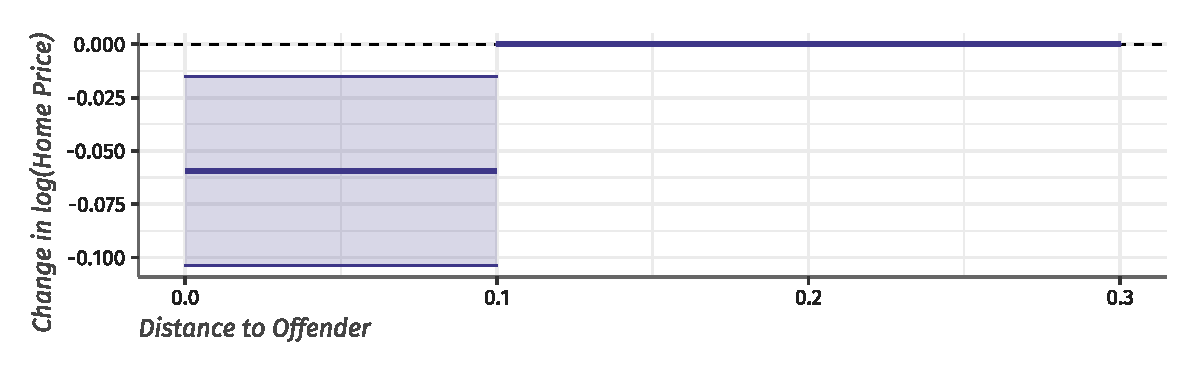
\includegraphics[width=\textwidth]{figures/geocoded/linden_rockoff_did.pdf}
    \end{subfigure}
    \hfill
    \begin{subfigure}{\textwidth}
        \caption{Nonparametric Approach}
        \centering
        \vspace{-2.5mm}
        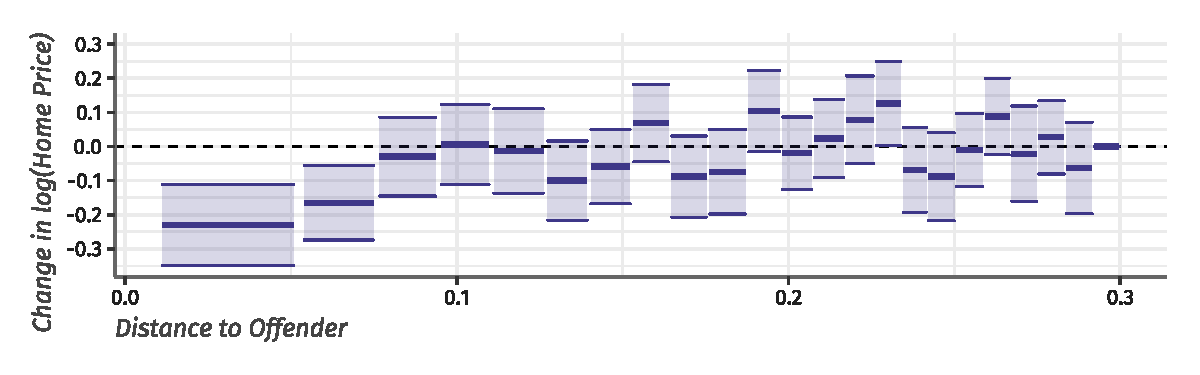
\includegraphics[width=\textwidth]{figures/geocoded/linden_rockoff.pdf}
    \end{subfigure}

    \note{This figure plots the estimated change in home prices after the arrival of a registered sex offender as a function of distance from offender. Each line plots $\hat{\tau}_j = \overline{\Delta Y}_j - \overline{\Delta Y}_l $ with associated standard errors. Panel (a) shows an estimate from Equation \ref{eq:ring_method} with a treatment distance of $1/10^{th}$ miles and a control distance of $1/3^{rd}$ mile. Panel (b) shows the nonparametric estimate of $\tau(\dist_i)$ proposed in Section \ref{sec:lspartition}.}
\end{figure}

Panel (b) of \autoref{fig:lr} applies the nonparametric approach described in Section \ref{sec:lspartition}. Two differences in results occur. First, homes in the two closest rings i.e. within a few hundred feet, are most affected by sex-offender arrival with an estimated decline of home value of around 20\%. homes a bit further away but still within in Linden and Rockoff's `treated' sample do not experience statistically significant treatment effects. As discussed above, Linden and Rockoff's estimate of $\bar{\tau}$ is attenuated towards zero because of the inclusion of homes with little to no treatment effects, leading them to understate the effect of arrival on home prices. The nonparametric approach improves on answering this question by providing a more complete picture of the treatment effect curve. The magnitude of treatment effects decrease over distance, providing additional evidence that the arrival causes a drop in home prices.\footnote{This is similar to estimating a dose-response function as evidence supporting a causal mechanism. The results of this paper are similar to the results of \citet{Callaway_Goodman-Bacon_SantAnna_2021} with continuous treatment. In their framework, \nameref{assum:parallel} is analagous to their assumption of common trends at different doses of a continuous treatment. In this setting, I am able to provide an estimator for the treatment effect curve, the average level effect in their terminology, by relying on an assumption that the treatment effect curve $\tau(\dist)$ is homogeneous across units.} 

The second advantage of this approach is that the produced figure provides an informal test of the local parallel trends assumption. After 0.1 miles, the estimated treatment effect curve becomes centered at zero consistently. This implies that units within each ring have the same estimated trend as the outer most ring, providing suggestive evidence that homes in this neighborhood are subject to the same trends. 

% ------------------------------------------------------------------------------
\section{Conclusion}
% ------------------------------------------------------------------------------

This article formalizes a common applied identification strategy that has a strong intuitive appeal. When treatment effects of shocks are experienced in only part of an area that would otherwise be on a common neighborhood-trend, difference-in-differences comparisons within a neighborhood can identify treatment effects. However, this paper shows that the typical \textit{estimator} for treatment effects requires a very strong assumption and returns only an average treatment effect among affected units when this assumption holds. 

This article then proposes an improved estimator that relies on nonparametric series estimators. The nonparametric estimator allows for estimation of the treatment effect at different distances from treatment, similar to a dose-response function, which can allow better understanding of \textit{who} is experiencing effects and how this changes across `exposure' to a shock. More, in some cases it can provide explanation for null results. For example, if a bus station creates negative externalities for apartments that border the station but positive externalities for apartments within walking distance, the average effect could be zero. However, nonparametric estimation would reveal the two effects seperately.


%-------------------------------------------------------------------------------
\bibliographystyle{apalike}
\bibliography{references}
%-------------------------------------------------------------------------------

%-------------------------------------------------------------------------------
\appendix
%-------------------------------------------------------------------------------

\chapter{Appendix to ``Dynamic Treatment Effect Estimation with Interactive Fixed Effects and Short Panels''}


% ------------------------------------------------------------------------------
\section{Proofs}\label{sec:generalized-proofs}
% ------------------------------------------------------------------------------



\subsection{Proof of \autoref{theorem:ATT_identification}}

Let $t \geq g$ for the given group $g$.

\begin{equation*}
    \expec{y_{it} - \bm P(\bm{F}_{t}', \bm{F}_{t < g}) \bm y_{i,t < g}}{G_i = g} = \expec{y_{it}(1)}{G_i = g} - \expec{\bm P(\bm{F}_{t}', \bm{F}_{t < g}) \bm y_{i,t < g}}{G_i = g} 
\end{equation*}
We use the fact that 
\begin{align*}
    \expec{ \bm P(\bm{F}_{t}', \bm{F}_{t < g}) \bm y_{i,t < g} }{G_i = g} 
    &= \expec{ \bm{F}_{t}' (\bm{F}_{t < g}' \bm{F}_{t < g})^{-1} \bm{F}_{t < g}' \bm y_{i,t < g} }{G_i = g} \\
    &= \expec{ \bm{F}_{t}' (\bm{F}_{t < g}' \bm{F}_{t < g})^{-1} \bm{F}_{t < g}' \big[\bm{F}_{t < g} \bm \gamma_i + u_{i,t < g} \big] }{G_i = g} \\
    &= \expec{ \bm{F}_{t}' \bm \gamma_i + \bm{F}_{t}' (\bm{F}_{t < g}' \bm{F}_{t < g})^{-1} \bm{F}_{t < g}' u_{i,t < g} }{G_i = g} \\
    &= \expec{ y_{it}(\infty) }{G_i = g} 
\end{align*}
The second equality hold by Assumption 2 and the fact that $y_{i,t < g} = y_{i, t < g}(0)$. The final equality holds by Assumption 2.

For the second part of the theorem, note that from the column span condition, there exists a $m \times p$ matrix $\bm A$ such that 
\begin{equation}
    \bm{F}^*\bm A = \bm{F}
\end{equation}
$\bm A$ defines the linear combinations of the columns of $\bm{F}^*$ that span the columns of $\bm{F}$. Thus $\bm{F}_t^{*'} \bm A = \bm{F}_t'$. We then have
\begin{align*}
    \bm{F}^{*'}_t (\bm{F}^{*'}_{t < g} \bm{F}^{*'}_{t < g})^{-1} \bm{F}^{*'}_{t < g} \bm{F}_{t < g} \bm \gamma_i
    &= \bm{F}^{*'}_t (\bm{F}^{*'}_{t < g} \bm{F}^{*}_{t < g})^{-1} \bm{F}^{*'}_{t < g} \bm{F}^{*'}_{t < g} \bm A \bm \gamma_i \\
    &= \bm{F}^{*'}_t \bm A \bm \gamma_i \\
    &= \bm{F}^{*'}_t \bm \gamma_i
\end{align*}

If $m = p$ so that $\bm{F}$ also has full column rank, we can make the stronger statement that the imputation matrices of $\bm{F}$ and $\bm{F}^{*}$ are equal: 
    \begin{align*}
        \bm P (\bm{F}_{t \geq g}, \bm{F}_{t < g}) 
        &= \bm{F}_{t \geq g} (\bm{F}_{t < g}' \bm{F}_{t < g})^{-1} \bm{F}_{t < g}' \\
        &= \bm{F}_{t \geq g} \bm A (\bm A'\bm{F}_{t < g}' \bm{F}_{t < g} \bm A)^{-1} \bm A' \bm{F}_{t < g}' \\
        &= \bm{F}^{*'}_{t \geq g} (\bm{F}^{*'}_{t < g} \bm{F}^{*}_{t < g})^{-1} \bm{F}^{*'}_{t < g} \\
        &= \bm P(\bm{F}^{*}_{t \geq g}, \bm{F}^{*}_{t < g})
    \end{align*}
    where the second equality holds because $\bm A$ and $(\bm{F}_{t < g}' \bm{F}_{t < g})$ are full rank.

$\square$

\subsection{Proof of \autoref{lemma:twfe_residuals}}

We first derive the averages defined in Section 2.2 in terms of the potential outcome framework:
\begin{gather*}
    \overline{y}_{\infty , t} = \frac{1}{N_{\infty}} \sum_{i = 1}^N D_{i \infty} y_{it} = \overline{\mu}_{\infty} + \lambda_t + \bm{F}_t \overline{\bm \gamma}_{\infty} + \overline{u}_{t, \infty}\\
    \overline{y}_{i,t\leq T_0} = \frac{1}{T_0} \sum_{t = 1}^{T_0} y_{it} = \mu_i + \overline{\lambda}_{t < T_0} + \overline{\bm{F}}_{t < T_0} \bm \gamma_i + \overline{u}_{i,t < T_0}\\
    \overline{y}_{\infty, t < T_0} = \frac{1}{N_{\infty} T_0} \sum_{i = 1}^N \sum_{t = 1}^{T_0} D_{i \infty} y_{it} = \overline{\mu}_{\infty} + \overline{\lambda}_{t < T_0} + \overline{\bm{F}}_{t < T_0} \overline{\bm \gamma}_{\infty} + \overline{u}_{\infty, t < T_0}
\end{gather*}
where $\overline{\mu}_{\infty}$ and $\overline{\bm \gamma}_{\infty}$ are the averages of the never-treated individuals' heterogeneity and $\overline{\bm{F}}_{t < T_0}$ and $\overline{\lambda}_{t < T_0}$ are the averages of the time effects before anyone is treated. The error averages have the same interpretation as the outcome averages.

The definition of $\tau_{it}$ is the difference between treated and untreated potential outcomes for unit $i$ at time $t$, so for any $(i,t)$, $y_{it} = d_{it} y_{it}(1) + (1-d_{it})y_{it}(\infty) = d_{it} \tau_{it} + y_{it}(\infty)$. Then
\begin{align*}
    \tilde{y}_{it} 
    &= d_{it} \tau_{it} + \bm{F}_t' \bm \gamma_i - \overline{\bm{F}}'_{t < T_0} \bm \gamma_i - \bm{F}_t' \overline{\bm \gamma}_{\infty} + \overline{\bm{F}}_{t < T_0} \overline{\bm \gamma}_{\infty} + u_{it} - \overline{u}_{t,\infty} - \overline{u}_{i, t < T_0} + \overline{u}_{\infty, t < T_0}\\
    &= d_{it} \tau_{it} + (\bm{F}_t - \overline{\bm{F}}_{t < T_0})' (\bm \gamma_i - \overline{\bm \gamma}_{\infty}) + u_{it} - \overline{u}_{t,\infty} - \overline{u}_{i, t < T_0} + \overline{u}_{\infty, t < T_0}
\end{align*}
Taking expectation conditional on $G_i = g$ gives $\expec{u_{it} - \overline{u}_{i, t < T_0}}{G_i = g} = 0$ by Assumption 2 and $\expec{\overline{u}_{\infty, t < T_0} - \overline{u}_{t, \infty} }{G_i = g} = \expec{\overline{u}_{\infty, t < T_0} - \overline{u}_{t, \infty}} = 0$ by random sampling and iterated expectations.

$\square$

\subsection{Proof of \autoref{theorem:ATT_identification}}

We can appeal to standard large sample GMM theory as in \citet{Hansen_1982} due to the types of first-stage factor estimators we consider. We do not consider true ``fixed effects" estimators where the number of parameters grows with the sample size. The IV and cross-sectional averages approaches are based on eliminating the factors (which are fixed in the asymptotic analysis) by reducing them to a smaller set of parameters. For example, while the CCE estimator can be implemented as a pooled regression where unit dummies are interacted with cross-sectional averages, the estimator itself takes a form similar to the within transformation in the linear fixed effects model. In fact, we prove asymptotic unbiasedness of dynamic ATT estimators using the CCE estimator in the first stage \citep{Brown_Butts_Westerlund_2023}\footnote{We consider CCE in a separate paper because the additional modeling assumptions allow for stronger results than those considered in this paper.}.

Consider the QLD estimator of \citet{Ahn_Lee_Schmidt_2013}. They study the linear model
\begin{equation}
    \bm y_i = \bm X_i \bm \beta + \bm F \bm \gamma_i + \bm \epsilon_i
\end{equation}
They jointly estimate the QLD parameters $\bm \theta$ along with the conditional response parameters $\bm \beta$ using the moment conditions
\begin{equation}
    \expec{\bm H(\bm \theta) (\bm y_i - \bm X_i \bm \beta) \otimes \bm w_i} = \bm 0
\end{equation}
They show that the estimator is well-behaved and does not suffer from asymptotic bias. As described in \citet{windmeijer2005finite}, the most likely source of finite-sample bias comes from estimating the optimal weight matrix. The appendix of \citet{Ahn_Lee_Schmidt_2013} describes a continuous updating estimator (CUE) based on their moment conditions, which may have less finite-sample bias than the optimal two-step estimator. However, we may also sacrifice efficiency in large samples if their assumed covariance structure is incorrect. 

We now derive the asymptotic variance of the full estimator under a general first-step estimator of the factors. Note that $\bm g_{i\infty}(\bm{\theta}) \otimes \bm g_{ig}(\bm{\theta}, \bm \tau_g) = \bm 0$ (from the $D_{ig}$ terms) and $\bm g_{ih}(\bm{\theta}, \bm \tau_h) \otimes \bm g_{ik}(\bm{\theta}, \bm \tau_k) = \bm 0$ almost surely uniformly over the parameter space for all $g \in \mathcal{G}$ and $h \neq k$. The covariance matrix of these moment functions, which we denote as $\bm \Delta$, is a block diagonal matrix.
\begin{equation*}
    \bm \Delta =
    \begin{pmatrix}
        \expec{\bm g_{i \infty}(\bm{\theta}) \bm g_{i \infty}(\bm{\theta})'} & \bm 0 & \bm 0 & \hdots & \bm 0\\
        \bm 0 &  \expec{\bm g_{i g_G}(\bm{\theta}, \bm \tau_{g_G}) \bm g_{i g_G}(\bm{\theta}, \bm \tau_{g_G})' } & \bm 0 & \hdots & \bm 0\\
        \vdots & & \ddots  &\\
        \bm 0 & \bm 0 & \bm 0 & \hdots & \expec{ \bm g_{i g_1}(\bm{\theta}, \bm \tau_{g_1}) \bm g_{i g_1}(\bm{\theta}, \bm \tau)'}
    \end{pmatrix}
\end{equation*}
We write the individual blocks as $\bm \Delta_g$ for $g \in \mathcal{G} \cup \{ \infty \}$. The gradient is also simple to compute because all of the moments are linear in the treatment effects. We define the overall gradient $\bm D$ and show it is a lower triangular matrix which we write in terms of its constituent blocks:
\begin{equation*}
    \bm D = 
    \begin{pmatrix}
        \expec{\nabla_{\bm{\theta}} \bm g_{i\infty}(\bm{\theta}) } & \bm 0 & \bm 0 & \hdots & \bm 0\\
        \expec{\nabla_{\bm{\theta}} \bm g_{ig_G}(\bm{\theta}, \bm \tau_{g_G})} & -\bm I_{T - g_G + 1} & \bm 0 & \hdots & \bm 0\\
        \vdots & & \ddots  &\\
        \expec{\nabla_{\bm{\theta}} \bm g_{ig_1}(\bm{\theta}, \bm \tau_{g_1})} & \bm 0 & \bm 0 & \hdots & -\bm I_{T - g_1 + 1}
    \end{pmatrix}
\end{equation*}
where we write the blocks in the first column as $\bm D_g$ for $g \in \mathcal{G} \cup \{ \infty \}$. The diagonal is made up of negative identity matrices because $\expec{\frac{D_{ig_h}}{\mathbb{P}(D_{ig_h} = 1)}} = 1$.

The overall asymptotic variance given that we use the optimal weight matrix is given by $(\bm D' \bm \Delta^{-1} \bm D)^{-1}$. $\bm\Delta$ is a block diagonal matrix so its inverse is trivial to compute. First, we have
\begin{equation*}
    \bm \Delta^{-1} \bm D = 
    \begin{pmatrix}
        \bm \Delta_{\infty}^{-1} \bm D_{\infty} & \bm 0 &  \hdots & \bm 0\\
        \bm \Delta_{g_G}^{-1} \bm D_{g_G} & -\bm \Delta_{g_G}^{-1} & \hdots & \bm 0\\
        \vdots & & \ddots &\\
        \bm \Delta_{g_1}^{-1} \bm D_{g_1} & \bm 0 & \hdots & - \bm \Delta_{g_1}^{-1}
    \end{pmatrix}
\end{equation*}
The transpose of the gradient matrix is
\begin{equation*}
    \bm D' =
    \begin{pmatrix}
        \bm D_{\infty}' & \bm D_{g_G}' & \hdots & \bm D_{g_1}'\\
        \bm 0 & -\bm I_{T-g_G + 1} & \hdots & \bm 0\\
        \vdots & & \ddots & \\
        \bm 0 & \bm 0 & \hdots & - \bm I_{T-g_1 + 1}
    \end{pmatrix}
\end{equation*}
so that we get
\begin{equation*}
    \bm D' \bm \Delta^{-1} \bm D = 
    \begin{pmatrix}
        \sum_{g \in \mathcal{G}\cup\{\infty\}} \bm D_g' \bm \Delta_g^{-1} \bm D_g & -\bm D_{g_G}' \bm \Delta_{g_G}^{-1} & \hdots & - \bm D_{g_1}' \bm \Delta_{g_G}^{-1}\\
        -\bm \Delta_{g_G}^{-1} \bm D_{g_G} & \bm \Delta_{g_G}^{-1} & \hdots & \bm 0\\
        \vdots & & \ddots &\\
        -\bm \Delta_{g_1}^{-1} \bm D_{g_1} & \bm 0 & \hdots & \bm \Delta_{g_1}^{-1}
    \end{pmatrix}
\end{equation*}

We write this matrix as 
\begin{equation*}
    \begin{pmatrix}
        \bm A & \bm B\\
        \bm C & \bm D
    \end{pmatrix}
\end{equation*}
where $\bm A = \sum_{g \in \mathcal{G}\cup \{\infty\}} \bm D_g' \bm \Delta_g^{-1} \bm D_g$ and $\bm D = \text{diag} \{ \bm \Delta_g^{-1} \}_{g \in \mathcal{G}}$. We then apply Exercise 5.16 of \citet{abadir2005matrix} to get the final inverse. The top left corner of the inverse is $\bm{F}^{-1}$ where
\begin{align*}
    (\bm{F})^{-1} 
    &= (\bm A - \bm B \bm D^{-1} \bm C)^{-1}\\
    &= \left( \sum_{g \in \mathcal{G}\cup\{\infty\}} \bm D_g' \bm \Delta_g^{-1} \bm D_g - \left( \sum_{g \in \mathcal{G}} \bm D_g' \bm \Delta_g^{-1} \bm D_g \right) \right)^{-1}\\
    &= (\bm D_{\infty}' \bm \Delta_{\infty}^{-1} \bm D_{\infty})^{-1}\\
    &= \text{Avar}(\sqrt{N}(\widehat{\bm{\theta}} - \bm{\theta}))
\end{align*}
The rest of the first column of matrices takes the form
\begin{align*}
    -\bm D^{-1} \bm C \bm{F}^{-1}
    &=
    \begin{pmatrix}
        \bm D_{g_G}\\
        \vdots\\
        \bm D_{g_1}
    \end{pmatrix}
    (\bm D_{\infty}' \bm \Delta_{\infty}^{-1} \bm D_{\infty})^{-1}\\
    &=
    \begin{pmatrix}
        \bm D_{g_G} (\bm D_{\infty}' \bm \Delta_{\infty}^{-1} \bm D_{\infty})^{-1}\\
        \vdots\\
        \bm D_{g_1} (\bm D_{\infty}' \bm \Delta_{\infty}^{-1} \bm D_{\infty})^{-1}
    \end{pmatrix}
\end{align*}
and the rest of the first row is $- \bm{F}^{-1} \bm B \bm D^{-1} = (- \bm D^{-1} \bm B' \bm{F}^{-1})' = (- \bm D^{-1} \bm C \bm{F}^{-1})'$.

Finally, the bottom-right block, which also gives the asymptotic covariance matrix of the ATT estimators, is 
\begin{align*}
    \bm D^{-1} + \bm D^{-1} \bm C \bm{F}^{-1} \bm B \bm D^{-1} 
    &= \bm D^{-1} + 
    \begin{pmatrix}
        \bm D_{g_G} (\bm D_{\infty}' \bm \Delta_{\infty}^{-1} \bm D_{\infty})^{-1} \bm D_{g_G}' & \hdots & \bm D_{g_G} (\bm D_{\infty}' \bm \Delta_{\infty}^{-1} \bm D_{\infty})^{-1} \bm D_{g_1}'\\
        & \ddots &\\
        \bm D_{g_1} (\bm D_{\infty}' \bm \Delta_{\infty}^{-1} \bm D_{\infty})^{-1} \bm D_{g_G}' & \hdots & \bm D_{g_1} (\bm D_{\infty}' \bm \Delta_{\infty}^{-1} \bm D_{\infty})^{-1} \bm D_{g_1}'
    \end{pmatrix}
\end{align*}
The $g$'th diagonal elements of the resulting matrix is $\bm \Delta_g + \bm D_g (\bm D_{\infty}' \bm \Delta_{\infty}^{-1} \bm D_{\infty})^{-1} \bm D_g'$.




$\square$




\subsection{Proof of \autoref{theorem:asymptotic_distribution}}

We derive the limiting theory by multiplying $\widehat{\bm \Delta}_g$ by $(N_g-1)/N_g$ which produces the same limit as $N \rightarrow \infty$. We write
\begin{equation*}
    \frac{N_g - 1}{ N_g} \widehat{\bm \Delta}_g = \frac{1}{N_g} \sum_{i = 1}^N D_{ig} \widehat{\bm \Delta}_{ig} \widehat{\bm \Delta}_{ig}' - \widehat{\bm \tau}_g \widehat{\bm \tau}_g'
\end{equation*}
We already know that $\widehat{\bm \tau}_g \plim \bm \tau_g$ by Theorem 3.1. Note that 
\begin{align*}
    \frac{1}{N_g} \sum_{i = 1}^N D_{ig} \widehat{\bm \Delta}_{ig} \widehat{\bm \Delta}_{ig}' = &\left( \frac{1}{N_g} \sum_{i = 1}^N D_{ig}  \bm y_{i, t \geq g} \bm y_{i, t \geq g}' \right) - \left( \frac{1}{N_g} \sum_{i = 1}^N D_{ig} \bm y_{i, t \geq g} \bm y_{i, t < g}' \right) \bm P(\bm{F}_{t \geq g}(\widehat{\bm{\theta}}), \bm{F}_{t < g}(\widehat{\bm{\theta}}))'\\
    &- \bm P(\bm{F}_{t \geq g}(\widehat{\bm{\theta}}), \bm{F}_{t < g}(\widehat{\bm{\theta}})) \left( \frac{1}{N_g} \sum_{i = 1}^N D_{ig} \bm y_{i, t < g} \bm y_{i, t \geq g}' \right)\\
    &- \bm P(\bm{F}_{t \geq g}(\widehat{\bm{\theta}}), \bm{F}_{t < g}(\widehat{\bm{\theta}})) \left( \frac{1}{N_g} \sum_{i = 1}^N D_{ig}  \bm y_{i, t < g} \bm y_{i, t \geq g}' \right) \bm P(\bm{F}_{t \geq g}(\widehat{\bm{\theta}}), \bm{F}_{t < g}(\widehat{\bm{\theta}}))'
\end{align*} 

Given $\bm P(\bm{F}_{t \geq g}(\widehat{\bm{\theta}}), \bm{F}_{t < g}(\widehat{\bm{\theta}}))$ is equal to its infeasible counterpart $\bm P(\bm{F}_{t \geq g}, \bm{F}_{t < g})$ plus a term that is $O_p(N^{-1/2})$, Assumption 1 and the weak law of large numbers imply 
\begin{equation*}
    \frac{1}{N_g} \sum_{i = 1}^N D_{ig} \widehat{\bm \Delta}_{ig} \widehat{\bm \Delta}_{ig}' - \widehat{\bm \tau}_g \widehat{\bm \tau}_g' \plim \expec{\bm g_{ig}(\bm{\theta}, \bm \tau_g)}{G_i = g} = \bm \Delta_g
\end{equation*}
The inverse exists with probability approaching one by Assumption 5.

$\square$

\section{The Quasi-Long-Differencing Estimator}

We discuss identification and inference of the imputation estimator using the QLD estimator for the factors. We derive the results here because QLD is used in both the simulations and application. 

\subsection{Identification}

We adapt the identifying assumptions from \citet{Ahn_Lee_Schmidt_2013} to our setup, guaranteeing Assumption \ref{asm:factor_identification} holds. Part (i) of the assumption holds assuming that $\bm F$ is full rank, because there always exists a matrix that applies Gaussian row-reduction to a full rank matrix. For parts (ii) and (iii), we need the following matrix to be full rank: 
\begin{equation}
    \bm I_{T-p} \otimes \expec{\bm w_i \bm \gamma_i'}{G_i = \infty}
\end{equation}
It implies that the instruments $\bm w_i$ are ``strong" in the sense that they correlate with the factor loadings $\bm \gamma_i$. Unfortunately, this restriction is not easily testable like in the case of two-stage least squares because the variable being instrumented for is unobserved. We leave the question of testing for instrument strength in quasi-differencing for a future project. Part (iv) is an additional assumption that is routinely made in practice. 

\subsection{Asymptotic Variance}

We now derive the analytical formulas for the asymptotic variance when quasi-differencing is used to estimate the factor space. Analytical standard errors can be obtained by replacing the population parameters with their estimators and expectations with the relevant sample average, e.g. expectations of the never-treated group are estimated using the average of the never-treated subsample. Conversely, one can average over the entire sample but multiply each observation by $D_{i\infty}$ and divide by $N_{\infty} / N$. To get the gradient of the set of moment conditions that identify the factor space, we rewrite the moment function as 
\begin{align*}
    \bm H(\bm \theta) \bm y_i \otimes \bm w_i
    &= \text{vec}(\bm w_i \bm y_i' \bm H(\bm \theta)')\\
    &= (\bm I_{(T-p)} \otimes \bm w_i \bm y_i') \bm K_{(T-p)T} \text{vec}(\bm H(\bm \theta))
\end{align*}
where $\bm K_{(T-p)T}$ is the $(T-p)T \times (T-p)T$ commutation matrix and we use the well-known relationship between vectorization and the Kronecker product\footnote{See Exercise 10.18 of \citet{abadir2005matrix}.}. Because $\text{vec}(\bm H(\bm \theta)) = [\text{vec}(\bm I_{T-p})', \bm \theta']'$, the gradient of the moment function is 
\begin{equation}
    \left( \bm I_{(T-p)} \otimes \bm w_i \bm y_i' \right) \bm K_{T(T-p)} [\bm 0_{(T-p)^2 \times (T-p)p}', \bm I_{(T-p)p}]'
\end{equation}
The expected gradient is obtained by taking expectations conditional on being in the never-treated group.

We now consider the gradient of the moment functions that determine the treatment effects with respect to the factor estimator for a given group treated at time $g$. The relevant part of the moment function for the purpose of finding the gradient is 
\begin{equation}
    \bm F_{t \geq g}(\bm \theta)' \left( \bm F_{t < g}(\bm \theta)' \bm F_{t < g}(\bm \theta) \right)^{-1} \bm F_{t < g}(\bm \theta)' \bm y_{i,t < g}
\end{equation}
There are two leading cases to compute: $g - 1 \geq T - p$ and $g - 1 < T - p$. In the first case, the parameters $\bm \theta$ are entirely contained in the pre-treatment factor matrix. Then 
\begin{equation}
    \bm F_{t < g} = 
    \begin{pmatrix}
        \bm \Theta\\
        \bm E
    \end{pmatrix}
\end{equation}
where $\bm E$ is the first $(g - 1) - (T - p)$ rows of $- \bm I_p$. Then the post-treatment factor matrix is just the lower $T - g + 1$ rows of $- \bm I_p$ so we do not need to worry about differentiating it. In this setting,
\begin{equation}
    \bm F_{t \geq g} \left( \bm F_{t < g}' \bm F_{t < g} \right)^{-1} \bm F_{t < g}' \bm y_{i,t < g} = - \left( \bm \Theta' \bm \Theta + \bm E' \bm E \right)^{-1} 
    \begin{pmatrix}
        \bm \Theta' & \bm E'
    \end{pmatrix}
    \bm y_{i,t < g}
\end{equation}
We use the notation in Chapter 13 of \citet{abadir2005matrix} to obtain the differential: 
\begin{align}
   - &
   \left( \bm \Theta' \bm \Theta + \bm E' \bm E \right)^{-1} 
    \begin{pmatrix}
        (d \bm \Theta)' & \bm E'
    \end{pmatrix}
    \bm y_{i,t < g}\\ 
    &
    \left( \bm \Theta' \bm \Theta + \bm E' \bm E \right)^{-1} \left( (d \bm \Theta)' \bm \Theta  \right) \left( \bm \Theta' \bm \Theta + \bm E' \bm E \right)^{-1}
    \begin{pmatrix}
        \bm \Theta' & \bm E'
    \end{pmatrix}
    \bm y_{i,t < g} \\
    &
    \left( \bm \Theta' \bm \Theta + \bm E' \bm E \right)^{-1} \left( \bm \Theta' (d \bm \Theta)  \right) \left( \bm \Theta' \bm \Theta + \bm E' \bm E \right)^{-1}
    \begin{pmatrix}
        \bm \Theta' & \bm E'
    \end{pmatrix}
    \bm y_{i,t < g} 
\end{align}
which can then be rewritten as 
\begin{align}
    -&
    \left( \bm y_{i,t < g} \otimes \left( \bm \Theta' \bm \Theta + \bm E' \bm E \right)^{-1} \right)     \begin{pmatrix}
        \bm K_{(T-p)p} (d \bm \theta)' & \bm K_{((g-1) - (T-p)p} \text{vec}(\bm E)'
    \end{pmatrix}'\\
    &
    \left( \left( \bm \Theta \left( \bm \Theta' \bm \Theta + \bm E' \bm E \right)^{-1}
    \begin{pmatrix}
        \bm \Theta' & \bm E'
    \end{pmatrix}
    \bm y_{i,t < g} \right)' \otimes \left( \bm \Theta' \bm \Theta + \bm E' \bm E \right)^{-1} \right) \bm K_{(T-p)p} d \bm \theta\\
    &
    \left( \left( \left( \bm \Theta' \bm \Theta + \bm E' \bm E \right)^{-1}
    \begin{pmatrix}
        \bm \Theta' & \bm E'
    \end{pmatrix}
    \bm y_{i,t < g} \right)' \otimes \left( \bm \Theta' \bm \Theta + \bm E' \bm E \right)^{-1} \bm \Theta' \right) d \bm \theta
\end{align}
The full gradient is then 
\begin{align}
    -&
    \left( \bm y_{i,t < g} \otimes \left( \bm \Theta' \bm \Theta + \bm E' \bm E \right)^{-1} \right)     \begin{pmatrix}
        \bm K_{(T-p)p}' & \bm 0_{((g-1) - (T-p)p \times (T-p)p} '
    \end{pmatrix}'\\
    &
    \left( \left( \bm \Theta \left( \bm \Theta' \bm \Theta + \bm E' \bm E \right)^{-1}
    \begin{pmatrix}
        \bm \Theta' & \bm E'
    \end{pmatrix}
    \bm y_{i,t < g} \right)' \otimes \left( \bm \Theta' \bm \Theta + \bm E' \bm E \right)^{-1} \right) \bm K_{(T-p)p}\\
    &
    \left( \left( \left( \bm \Theta' \bm \Theta + \bm E' \bm E \right)^{-1}
    \begin{pmatrix}
        \bm \Theta' & \bm E'
    \end{pmatrix}
    \bm y_{i,t < g} \right)' \otimes \left( \bm \Theta' \bm \Theta + \bm E' \bm E \right)^{-1} \bm \Theta' \right)
\end{align}
when $g - 1 \geq T-p$. 

The second case, when $g - 1 < T-p$, now has parameters in the post-treatment matrix $\bm F_{t \geq g}$. We redefine the parameters as $\bm \Theta = [ \bm \Theta_1', \bm \Theta_2']'$ where $\bm \Theta_1$ is $(g-1) \times p$ and $\bm \Theta_2$ is $(T-p - g + 1) \times p$. Now we write $\bm F_{t < g} = \bm \Theta_1$ and 
\begin{equation}
    \bm F_{t \geq g} = 
    \begin{pmatrix}
        \bm \Theta_2\\
        - \bm I_p
    \end{pmatrix}
\end{equation}
Because $\bm \theta \neq (\text{vec}(\bm \Theta_1)', \text{vec}(\bm \Theta_2)')'$, we define the matrices $\bm E_1 = [\bm I_{g-1}, \bm 0_{(g-1) \times (T-p - g+1)}$ and $\bm E_2 = [ \bm 0_{(T-p - g + 1) \times (g-1)}, \bm I_{(T-p -g + 1)}]$ such that 
\begin{gather}
    \bm \Theta_1 = \bm E_1 \bm \Theta\\
    \bm \Theta_2 = \bm E_2 \bm \Theta
\end{gather}
Now we can rewrite the relevant portion of the moment function for the gradient as
\begin{equation}
    \begin{pmatrix}
        \bm E_2 \bm \Theta\\
        -\bm I_p
    \end{pmatrix}
    \left( \bm \Theta' \bm E_1' \bm E_1 \bm \Theta \right)^{-1} \bm \Theta' \bm E_1' \bm y_{i, t < g}
\end{equation} 
We can now take the gradient with respect to the full set of parameters $\bm \theta$:
\begin{align}
    & 
    \begin{pmatrix}
        \bm E_2 d \bm \Theta\\
        \bm 0_{p \times p}
    \end{pmatrix}
    \left( \bm F_{t < g}' \bm F_{t < g} \right)^{-1} \bm F_{t < g}' \bm y_{i, t < g}\label{case2_diff_eq1}\\
    - & 
    \bm F_{t \geq g} \left( \bm F_{t < g}' \bm F_{t < g} \right)^{-1} d \bm \Theta' \bm E_1' \bm F_{t < g} \left( \bm F_{t < g}' \bm F_{t < g} \right)^{-1} \bm F_{t < g}' \bm y_{i, t < g}\\
    - & \bm F_{t \geq g} \left( \bm F_{t < g}' \bm F_{t < g} \right)^{-1} \bm F_{t < g}' \bm E_1 d \bm \Theta \left( \bm F_{t < g}' \bm F_{t < g} \right)^{-1} \bm F_{t < g}' \bm y_{i, t < g}\\
    + & 
    \bm F_{t \geq g} \left( \bm F_{t < g}' \bm F_{t < g} \right)^{-1} d \bm \Theta' \bm E_1' \bm y_{i, t < g}
\end{align}
where we inserted $\bm F_{t < g}$ and $\bm F_{t \geq g}$ for $\bm E_1 \bm \Theta$ and $\bm E_2 \bm \Theta$ respectively to preserve space, noting that these matrices are actually functions of the parameters $\bm \theta$ and not the true, unobserved factors. We rewrite line \eqref{case2_diff_eq1} so we can write the differential in terms of $\bm \theta$: 
\begin{align}
    \begin{pmatrix}
        \bm E_2 d \bm \Theta\\
        \bm 0_{p \times p}
    \end{pmatrix}
    \left( \bm F_{t < g}' \bm F_{t < g} \right)^{-1} \bm F_{t < g}' \bm y_{i, t < g} 
    &= 
    \begin{pmatrix}
        \bm E_2\\
        \bm 0_{p \times p}
    \end{pmatrix}
    d \bm \Theta
    \left( \bm F_{t < g}' \bm F_{t < g} \right)^{-1} \bm F_{t < g}' \bm y_{i, t < g}\\
    &=
    \left( \left( \left( \bm F_{t < g}' \bm F_{t < g} \right)^{-1} \bm F_{t < g}' \bm y_{i, t < g} \right) \otimes 
        \begin{pmatrix}
        \bm E_2\\
        \bm 0_{p \times p}
    \end{pmatrix}
    \right)
    d \bm \theta
\end{align}
We put this expression with the others to get the final gradient: 
\begin{align}
    &= \left( \left( \bm F_{t < g}' \bm F_{t < g} \right)^{-1} \bm F_{t < g}' \bm y_{i, t < g} \right) \otimes 
        \begin{pmatrix}
        \bm E_2\\
        \bm 0_{p \times p}
    \end{pmatrix}\\
    &
    - \left( \bm E_1' \bm F_{t < g} \left( \bm F_{t < g}' \bm F_{t < g} \right)^{-1} \bm F_{t < g}' \bm y_{i,t < g} \right)' \otimes \left( \bm F_{t \geq g} \left( \bm F_{t < g}' \bm F_{t < g} \right)^{-1} \right) \bm K_{(T-p)p}\\
    &
    - \left( \left( \bm F_{t < g}' \bm F_{t < g} \right)^{-1} \bm F_{t < g}' \bm y_{i,t < g} \right)' \otimes \left( \bm F_{t \geq g} \left( \bm F_{t < g}' \bm F_{t < g} \right)^{-1} \bm F_{t < g}' \bm E_1 \right)\\
    &
    + \left( \bm y_{i,t < g}' \bm E_1 \right) \otimes \left( \bm F_{t \geq g} \left( \bm F_{t < g}' \bm F_{t < g} \right)^{-1} \right) \bm K_{(T-p)p}
\end{align}


% \nick{3/5/2024: The work on the second case below is old and I don't think it works as well as the argument above. I want to make sure I get everything in line. }

% The second case, when $g - 1 < T-p$, now has parameters in the post-treatment matrix $\bm F_{t \geq g}$. We redefine the parameters as $\bm \Theta = [ \bm \Theta_1', \bm \Theta_2']'$ where $\bm \Theta_1$ is $(g-1) \times p$ and $\bm \Theta_2$ is $((T-p) - (g-1) + 1) \times p$. Now we write $\bm F_{t < g} = \bm \Theta_1$ and 
% \begin{equation}
%     \bm F_{t \geq g} = 
%     \begin{pmatrix}
%         \bm \Theta_2\\
%         - \bm I_p
%     \end{pmatrix}
% \end{equation}
% so that the relevant portion of the moment function that identifies the ATTs for group $g$ is 
% \begin{equation}\label{second_case_moment_fn}
%     \begin{pmatrix}
%         \bm \Theta_2\\
%         - \bm I_p
%     \end{pmatrix}
%     \left( \bm \Theta_1' \bm \Theta_1 \right)^{-1} \bm \Theta_1' \bm y_{t < g} = 
%     \begin{pmatrix}
%         \bm \Theta_2 \left( \bm \Theta_1' \bm \Theta_1 \right)^{-1} \bm \Theta_1' \bm y_{t < g}\\
%         - \left( \bm \Theta_1' \bm \Theta_1 \right)^{-1} \bm \Theta_1' \bm y_{t < g}
%     \end{pmatrix}
% \end{equation}
% The gradient with respect to $\bm \Theta_2$ can be shown to be 
% \begin{equation}
%     \begin{pmatrix}
%         \left( \left( \bm \Theta_1' \bm \Theta_1 \right)^{-1} \bm \Theta_1' \bm y_{t < g} \right)' \otimes \bm I_{g-1}\\
%         \bm 0_{p \times ((T-p) - (g-1) + 1)p}
%     \end{pmatrix}
% \end{equation}
% Rewriting equation \eqref{second_case_moment_fn} as $\bm F_{t \geq g} \left( \bm \Theta_1' \bm \Theta_1 \right)^{-1} \bm \Theta_1' \bm y_{t < g}$, we can easily calculate the gradient using the argument from the first case as
% \begin{align}
%     & \bm F_{t \geq g} \left( \bm y_{i,t < g} \otimes (\bm \Theta_1' \bm \Theta_1)^{-1} \right) \\
%     - & \bm F_{t \geq g} \left( \left( (\bm \Theta_1' \bm \Theta_1)^{-1} \bm \Theta_1' \bm y_{i, t < g} \right)' \otimes (\bm \Theta_1' \bm \Theta_1)^{-1} \right) \bm K_{(g-1) p}\\
%     - & \bm F_{t > g} \left( \left( (\bm \Theta_1' \bm \Theta_1)^{-1} \bm \Theta_1' \bm y_{i,t<g} \right)' \otimes (\bm \Theta_1' \bm \Theta_1)^{-1} \bm \Theta_1' \right)
% \end{align}
% \nick{3/4/2024: Again, need to double check all this stuff. Also need to find the linear transformation that turns $(\bm \theta_1', \bm \theta_2')' \rightarrow \bm \theta$.}


% ------------------------------------------------------------------------------
\section{Inference of Aggregate Treatment Effects}
% ------------------------------------------------------------------------------

As in \citet{Callaway_Santanna_2021}, we can form aggregates of our group-time average treatment effects. For example, event-study type coefficients would average over the $\tau_{gt}$ where $t - g = e$ for some relative event-time $e$ with weights proportional to group membership. Consider a general aggregate estimand $\delta$ which we define as a weighted average of $ATT(g,t)$:
\begin{equation}
\delta = \sum_{g\in \mathcal{G}} \sum_{t > T_0} w(g,t) \tau_{gt}
\end{equation}
where the weights $w(g,t)$ are non-negative and sum to one. Table 1 of \citet{Callaway_Santanna_2021} and the surrounding discussion describes various treatment effect aggregates and discuss explicit forms for the weights. 

Our plug-in estimate for $\delta$ is given by $\hat{\delta} = \sum_{g\in \mathcal{G}} \sum_{t > T_0} \hat{w}(g,t) \hat{\tau}_{gt}$. Inference on this term follows directly from Corollary 2 in \citet{Callaway_Santanna_2021} if we have the influence function for our $\tau_{gt}$ estimates. Rewriting our moment equations in an asymptotically linear form, we have:
\begin{equation}
    \sqrt{N}\Big( (\widehat{\bm{\theta}}', \widehat{\bm \tau}')' - (\bm{\theta}', \bm \tau')' \Big) = - \left( \frac{1}{\sqrt{N}} \sum_{i = 1}^N (\bm D' \bm \Delta^{-1} \bm D)^{-1} \bm D' \bm \Delta^{-1} \bm g_i(\bm{\theta}, \bm \tau) \right) + o_p(1).
\end{equation}
This form comes from the fact that the weight matrix is positive definite with probability approaching one\footnote{This is a well-known expansion for analyzing the asymptotic properties of GMM estimators. See Chapter 14 of \citet{Wooldridge_2010} for example.}. The first term on the right-hand side is the influence function and hence inference on aggregate quantities follows directly. This result allows for use of the multiplier bootstrap to estimate standard errors in a computationally efficient manner.

% ------------------------------------------------------------------------------
\section{Inference in Two-Way Fixed Effect Model}\label{sec:twfe_inference}
% ------------------------------------------------------------------------------

We derive the asymptotic distribution of our imputation estimator based off of the two-way error model in equation (1). First, we note that this estimator can be written in terms of the imputation matrix from Section 2. In particular, let $\bm 1_t$ be a $T \times 1$ vector of ones up the $t$'th spot, with all zeros after. Define $\overline{\bm y}_{\infty} = (\overline{y}_{\infty, 1},..., \overline{y}_{\infty, T})'$ be the full vector of never-treated cross-sectional averages. Then our imputation transformation can be written as 
\begin{equation}
    \tilde{\bm y}_i = \left[ \bm I_T - \bm P(\bm 1_T, \bm 1_{T_0}) \right] (\bm y_i - \overline{\bm y}_{\infty})
\end{equation}
where the $t^{th}$ component of the above $T$-vector is 
\begin{equation}
    d_{it} \tau_{it} + \tilde{u}_{it},
\end{equation}
with $\tilde{u}_{it}$ is defined as the same transformation as $\tilde{y}_{it}$.

The imputation step of our estimator is a just-identified system of equations. As such, we do not need to worry about weighting in implementation and inference comes from standard theory of M-estimators. In fact, we have the following closed-form solution for the estimator of a group-time average treatment effect: 
\begin{equation}
    \widehat{\tau}_{gt} = \frac{1}{N_{g}}\sum_{i} D_{ig} \tilde{y}_{it},
\end{equation}
where $N_{g} = \sum_i D_{ig}$ is the number of units in group $g$. 

The following theorem characterizes estimation under the two-way error model:
\begin{theorem}\label{theorem:twfe}
    Assume untreated potential outcomes take the form of the two-way error model given in equation (1). Suppose Assumptions 1 and 3 hold, as well as Assumption 2 with $\bm \gamma_i = 0$. Then for all $(g, t)$ with $g > t$, $\widehat{\bm \tau}_{gt}$ is conditionally unbiased for $\expec{\tau_{it}}{D_{ig} = 1}$, has the linear form
    \begin{equation}\label{eq:twfe_influence}
        \sqrt{N_{g}} \big( \widehat{\tau}_{gt} - \tau_{gt} \big) 
        = \frac{1}{\sqrt{N_{g}}}\sum_{i=1}^N D_{ig} (\tau_{it} - \tau_{gt} + u_{it} - \overline{u}_{i,t < T_0} - \overline{u}_{\infty,t} + \overline{u}_{\infty,t < T_0})
    \end{equation}
    and  
    \begin{equation}\label{eq:twfe_asymptotic}
        \sqrt{N_1}(\widehat{\tau}_{gt} - \tau_{gt}) \convd N(0, V_1 + V_0)
    \end{equation}
    as $N \rightarrow \infty$, where $V_1$ and $V_0$ are given below and $\tau_{gt} = \expec{y_{it}(g) - y_{it}(\infty)}{D_{ig} = 1}$ is the group-time average treatment effect (on the treated). $\blacksquare$
\end{theorem}
Theorem (\ref{theorem:twfe}) demonstrates the simplicity of our imputation procedure under the two-way error model. While the general factor structure requires more care, estimation and inference will yield a similar result.


\subsection{Proof of Theorem \autoref{theorem:twfe}}

The transformed post-treatment observations are
\begin{equation}
    \tilde{y}_{it} = \tau_{it} + u_{it} - \overline{u}_{\infty,t}  - \overline{u}_{i,t < T_0} + \overline{u}_{\infty,t < T_0}
\end{equation}
To show unbiasedness, take expectation conditional on $D_{ig} = 1$. This expected value is
\begin{equation}
    \expec{ \tau_{it} + u_{it} - \overline{u}_{i,t < T_0} - \overline{u}_{\infty,t} + \overline{u}_{\infty,t < T_0} }{D_{ig} = 1} = \expec{\tau_{it}}{D_{ig} = 1}
\end{equation}
by Assumption 2 and 3.

For consistency, note that averaging over the sample with $D_{ig} = 1$, subtracting $\tau_{gt}$, and multiplying $\sqrt{N_{g}}$ gives
\begin{align}
    \sqrt{N_{g}} \big( \widehat{\tau}_{gt} - \tau_{gt} \big) 
    = \frac{1}{\sqrt{N_{g}}}\sum_{i=1}^N D_{ig} (\tau_{it} - \tau_{gt} + u_{it} - \overline{u}_{i,t < T_0})
    + \frac{1}{\sqrt{N_{g}}}\sum_{i = 1}^N D_{ig} (- \overline{u}_{\infty,t} + \overline{u}_{\infty,t < T_0}) 
\end{align}
which is two normalized sums of uncorrelated iid sequences that have mean zero (by iterated expectations) and finite fourth moments. % The right-hand side is the influence function for $\tau_{gt}$ so inference across terms is possible as well as inference for aggregates following \citet{Callaway_Santanna_2021}.

Rewriting the second term in terms of the original averages $\frac{1}{N_\infty} \sum_{i=1}^N - u_{i,t} + \overline{u}_{i,t < T_0}$ gives:
\begin{align*}
    \sqrt{N_{g}} \big( \widehat{\tau}_{gt} - \tau_{gt} \big) 
    &= \frac{1}{\sqrt{N_{g}}}\sum_{i=1}^N D_{ig} (\tau_{it} - \tau_{gt} + u_{it} - \overline{u}_{i,t < T_0}) \\
    &\quad + \sqrt{\frac{N_g}{N_\infty}} \bigg ( \frac{1}{\sqrt{N_\infty}} \sum_{i = 1}^N D_{i\infty} (- u_{i,t} + \overline{u}_{i,t < T_0} ) \bigg)
\end{align*}
Since these terms are mean zero and uncorrelated, we find the variance of each term separately. 

The first term has asymptotic variance 
\begin{equation}
V_1 = \expec{\Big( \tau_{it} - \tau_{gt} + u_{it} - \overline{u}_{i,t < T_0} \Big) \Big( \tau_{it} - \tau_{gt} + u_{it} - \overline{u}_{i,t < T_0} \Big)'}{D_{ig} = 1}
\end{equation}
and the second term has asymptotic variance
\begin{equation}
V_0 = \frac{\mathbb{P}(D_{ig} = 1)}{\mathbb{P}(D_{i\infty} = 1)} \expec{ \Big( \overline{u}_{i,t < T_0} - u_{i,t} \Big) \Big( \overline{u}_{i,t < T_0} - u_{i,t} \Big)' }{D_{i\infty} = 1}
\end{equation}
The result follows from the independence of the two sums.




\section{Including Covariates}

%11/29/2022 draft

We now discuss the inclusion of covariates in the untreated potential outcome mean model. Allowing for covariates further weakens our parallel trends assumption by allowing selection to hold on unobserved heterogeneity as well as observed characteristics. Identifying the effects of covariates requires some kind of time and unit variation because we manually remove the level fixed effects. 

A common inclusion in the treatment effects literature is time-constant variables with time-varying slopes. Suppose $\bm x_i$ is $1 \times K$ vector of time-constant covariates. We could write the mean model of the untreated outcomes as 
\begin{equation}
    \expec{y_{it}(\infty)}{x_i, \mu_i, \bm \gamma_i, D_i} = \bm x_i \bm \beta_t + \mu_i + \lambda_t + \bm{F}_t' \bm \gamma_i
\end{equation}
which allows observable covariates to have trending partial effects; covariates with constant slopes are captured by the unit effect. After removing the additive fixed effects, $\bm x_i \bm \beta_t$ will take the same form as the residuals of factor structure. Estimating $\bm{\theta}$ can be done jointly with the time-varying coefficients by applying the QLD transformation to the vector of $\tilde{y}_{it} - \tilde{x}_i \tilde{\beta}_t$. We cannot identify the underlying partial effects because of the time-demeaning, but we can include them for the sake of strengthening the parallel trends assumption.

Time-constant covariates (or time-varying covariates fixed at their pre-treatment value) are often employed because there is little worry that they are affected by treatment. However, we could also include time- and individual-varying covariates of the form $\bm x_{it}$ that are allowed to have identifiable constant slopes if we assume their distribution is unaffected by treatment status. Let $\bm x_{it}$ be a $1 \times K$ vector of covariates that vary over $i$ and $t$. We can jointly estimate a $K \times 1$ vector of parameters $\bm \beta$ along with $\bm{\theta}$ using the moments
\begin{equation}
    \expec{\bm H(\bm{\theta})' (\tilde{\bm y_i} - \tilde{\bm X_i} \bm \beta) \otimes \bm w_i}{G_i = \infty} = \bm 0
\end{equation}
where $\Tilde{\bm X}_i$ is the $T \times K$ matrix of stacked covariates after our double-demeaning procedure.

We could also allow slopes to vary across groups and estimate them via the group-specific pooled regression $D_{ig} y_{it}$ on $D_{ig} \bm x_{it}$ with unit-specific slopes on $D_{ig} \Tilde{\bm{F}}(\widehat{\bm{\theta}})_t$ for $t = 1,..., g-1$. Then we include the covariates and their respective slopes into the moment conditions
\begin{equation}
    \expec{(\tilde{\bm y}_{i,t\geq g} - \tilde{\bm X}_{i, t \geq g} \bm \beta_g) - \bm P(\tilde{\bm{F}}_{t \geq g}, \tilde{\bm{F}}_{t < g}) (\tilde{\bm y}_{i,t< g} - \tilde{\bm X}_{i, t < g} \bm \beta_g) - \bm \tau_g  }{G_i = g} = \bm 0
\end{equation}
We note that the above expression requires treatment to not affect the evolution of the covariates, a strong assumption in practice. \citet{Chan_and_Kwok_2022} make a similar assumption for their principal components difference-in-differences estimator. We study this assumption in the context of the common correlated effects model in \citet{Brown_Butts_Westerlund_2023}.


\section{Testing Mean Equality of Factor Loadings}

We develop this test in the context of the QLD estimation of \citet{Ahn_Lee_Schmidt_2013}. Specifically, we need $\expec{\bm \gamma_i} = \expec{\bm \gamma_i}{G_i = g}$ for all $g \in \mathcal{G}$. Our imputation approach allows us to identify these terms up to a rotation. To see how, let $\bm A^*$ be the rotation that imposes the \citet{Ahn_Lee_Schmidt_2013} normalization. Then
\begin{align*}
    \bm P(\bm I_{p}, \bm{F}(\bm{\theta})_{t < g}) \expec{\bm y_{i, t < g}}{G_i = g} 
    &= \left( \bm{F}(\bm{\theta})_{t < g}' \bm{F}(\bm{\theta})_{t < g} \right)^{-1} \bm{F}(\bm{\theta})_{t < g}' \bm{F}_{t < g} \expec{\bm \gamma_i}{G_i = g}\\
    &= \left( \bm{F}(\bm{\theta})_{t < g}' \bm{F}(\bm{\theta})_{t < g} \right)^{-1} \bm{F}(\bm{\theta})_{t < g}' \bm{F}(\bm{\theta})_{t < g} (\bm A^*)^{-1} \expec{\bm \gamma_i}{G_i = g}\\
    &= (\bm A^*)^{-1} \expec{\bm \gamma_i}{G_i = g}
\end{align*}
where $\bm{F}(\bm{\theta}) = \bm{F} \bm A^*$.

It is irrelevant that the means of the factor loadings are only known up to a nonsingular transformation, because $\bm A^*$ is the same for each $g \in \mathcal{G}$ by virtue of the common factors. We note that
\begin{equation}
    \expec{\bm \gamma_i}{G_i = g} - \expec{\bm \gamma_i} = \bm 0 \iff (\bm A^*)^{-1}(\expec{\bm \gamma_i}{G_i = g} - \expec{\bm \gamma_i}) = \bm 0
\end{equation}
The results above show how we can identify $(\bm A^*)^{-1} \expec{\bm \gamma_i}{G_i = g}$ by imputing the pre-treatment observations onto an identify matrix. 

Collect the moments 
\begin{gather*}
    \expec{\frac{D_{i \infty}}{\mathbb{P}(D_{i \infty} = 1)}\bm H(\bm{\theta}) \tilde{\bm y}_i \otimes \bm w_i} = \bm 0\\
    \expec{\frac{D_{i \infty}}{\mathbb{P}(D_{i \infty} = 1)} \left( \bm P(\bm I_p, \bm{F}(\bm{\theta})) \bm y_i - \bm \gamma^* \right)} = \bm 0\\
    \expec{\frac{D_{i g_G}}{\mathbb{P}(D_{ig_G} = 1)} \left( \bm P(\bm I_p, \bm{F}(\bm{\theta})_{t < g_G}) \bm y_{i,t < g_G} - \bm \gamma_{g_G}^* \right) } = \bm 0\\
    \vdots\\
    \expec{\frac{D_{i g_1}}{\mathbb{P}(D_{ig_1} = 1)} \left( \bm P(\bm I_p, \bm{F}(\bm{\theta})_{t < g_1}) \bm y_{i,t < g_1} - \bm \gamma_{g_G}^* \right) } = \bm 0
\end{gather*}
The parameters $(\bm \gamma^*, \bm \gamma_{g_G}^*,...,\bm \gamma_{g_1}^*)$ represent the rotated means of the factor loadings. $\bm \gamma$ is the unconditional mean $(\bm A^*)^{-1}\expec{\bm \gamma_i}$ and $\bm \gamma_g$ is the conditional mean $(\bm A^*)^{-1}\expec{\bm \gamma_i}{G_i = g}$ for $g \in \mathcal{G}$. We include estimation of the factors for convenience, so that one does not need to directly calculate the effect of first-stage estimation on the asymptotic variances of conditional means. 

Joint GMM estimation of the above parameters, including $\bm{\theta}$, then allows one to test combinations of the rotated means. Specifically, we have the following result: 
\begin{theorem}
    If $\expec{\bm \gamma_i}{G_i = g} = \expec{\bm \gamma_i}$ for all $g \in \mathcal{G}$, then
    \begin{equation}
        \bm \gamma^* = \bm \gamma_{g_G}^* = ... = \bm \gamma_{g_1}^*
    \end{equation}
    $\blacksquare$
\end{theorem}

\chapter{Appendix to ``Difference-in-Differences with Spatial Spillovers''}

% ------------------------------------------------------------------------------
\section{Proofs}
\label{sec:spillover-proofs}
% ------------------------------------------------------------------------------

% ------------------------------------------------------------------------------
\subsection{Proof of Proposition \ref{prop:bias}}
% ------------------------------------------------------------------------------

\begin{align*}
    &\underbrace{\expec{Y_{i1} - Y_{i0} \mid D_i = 1 } - \expec{Y_{i1} - Y_{i0} \mid D_i = 0 }}_{\text{Difference-in-Differences}} \\
    &= \expec{Y_{i1}(1, h_i(\bm{D})) - Y_{i0}(0, \bm{0})  \mid D_i = 1 } - \expec{Y_{i1}(0, h_i(\bm{D})) - Y_{i0}(0, \bm{0}) \mid D_i = 0 } \\
    % &= \expec{Y_{i1}(1, h_i(\bm{D})) - Y_{i0}(0, \bm{0})  \mid D_i = 1 } \\
    % &\quad\quad - \expec{Y_{i1}(0, h_i(\bm{D})) + Y_{i1}(0, \bm{0}) - Y_{i1}(0, \bm{0}) - Y_{i0}(0, \bm{0}) \mid D_i = 0 } \\
    &= \expec{Y_{i1}(1, h_i(\bm{D})) - Y_{i0}(0, \bm{0})  \mid D_i = 1 } - \expec{Y_{i1}(0, \bm{0}) - Y_{i0}(0, \bm{0}) \mid D_i = 0} \\ 
    &\quad\quad - \expec{Y_{i1}(0, h_i(\bm{D})) - Y_{i1}(0, \bm{0})\mid D_i = 0} \\ 
    &= \expec{Y_{i1}(1, h_i(\bm{D})) - Y_{i0}(0, \bm{0})  \mid D_i = 1 } - \expec{Y_{i1}(0, \bm{0}) - Y_{i0}(0, \bm{0}) \mid D_i = 1} \\
    &\quad\quad - \expec{Y_{i1}(0, h_i(\bm{D})) - Y_{i1}(0, \bm{0})\mid D_i = 0} \\  
    % &= \expec{Y_{i1}(1, h_i(\bm{D})) - Y_{i0}(0, \bm{0}) - Y_{i1}(0, \bm{0}) + Y_{i0}(0, \bm{0})\mid D_i = 1 } \\
    % &\quad\quad - \expec{Y_{i1}(0, h_i(\bm{D})) - Y_{i1}(0, \bm{0})\mid D_i = 0}\\
    &= \expec{Y_{i1}(1, h_i(\bm{D})) - Y_{i1}(0, \bm{0}) \mid D_i = 1 } - \expec{Y_{i1}(0, h_i(\bm{D})) - Y_{i1}(0, \bm{0})\mid D_i = 0} \\
    &\equiv \tau_{\text{total}} - \tau_{\text{spill}}(0), 
\end{align*}
where the first equality comes from the potential outcomes and the \nameref{assumption:no-anticipation} assumption, the second from adding and subtracting terms, the third equality follows from the \nameref{assumption:parallel} assumption, and the final equality follows from the definitions of total and spillover effects.

% ------------------------------------------------------------------------------
\subsection{Proof of Proposition \ref{prop:total_effect}}
% ------------------------------------------------------------------------------

\begin{align*}
    &\expec{Y_{i1} - Y_{i0} \ \mid \ D_i = 1} - \expec{Y_{i1} - Y_{i0} \ \mid \ D_i = 0, S_i =0} \\
    &\quad\quad= \expec{Y_{i1}(1, h_i(\bm{D})) - Y_{i0}(0, \bm{0}) \ \mid \ D_i = 1} - \expec{Y_{i1}(0, \bm{0}) - Y_{i0}(0, \bm{0}) \ \mid \ D_i = 0, S_i =0} \\
    &\quad\quad= \expec{Y_{i1}(1, h_i(\bm{D})) - Y_{i0}(0, \bm{0}) \ \mid \ D_i = 1} - \expec{Y_{i1}(0, \bm{0}) - Y_{i0}(0, \bm{0}) \ \mid \ D_i = 1} \\
    &\quad\quad= \expec{Y_{i1}(1, h_i(\bm{D})) - Y_{i0}(0, \bm{0}) - Y_{i1}(0, \bm{0}) + Y_{i0}(0, \bm{0}) \ \mid \ D_i = 1} \\
    &\quad\quad= \expec{Y_{i1}(1, h_i(\bm{D})) - Y_{i1}(0, \bm{0}) \ \mid \ D_i = 1} \\
    &\quad\quad\equiv \tau_{\text{total}},
\end{align*}
where the first equality comes from the fact that $S_i = 0$ implies $h_i(\bm{D}) = 0$, the second equality from parallel trends assumption (\ref{assumption:parallel-mod}), and the last by definition of the total effect.



% ------------------------------------------------------------------------------
\subsection{Identification of Imputation Estimator}\label{sec:identification_imputation}
% ------------------------------------------------------------------------------

This section will give identification arguments for the total effect and spillover effects. First, note under \nameref{assumption:parallel_staggered}, we have 
\begin{align*}
  \expec{Y_{it}(d_{it}, h_i(\bm{D}_t)) - \mu_i - \lambda_t \ | \ d_{it} = 1} 
  &= \expec{\tau_{it}(d_{it}, h_i(\bm{D}_t)) + \varepsilon_{it} \ | \ d_{it} = 1} \\
  &= \expec{\tau_{it}(d_{it}, h_i(\bm{D}_t)) \ | \ d_{it} = 1} \\
  &= \tau_{total}.
\end{align*}
In the first stage, we estimate $\mu_i$ and $\lambda_t$ using observations with $d_{it}$ and $S_{it} = 0$. Unbiasedness/consistency follows from \nameref{assumption:local} and \nameref{assumption:no-anticipation_staggered} and the arguments of the appendix of \citet{Gardner_2021}.

A similar argument follows for spillover effects. Again, assuming \nameref{assumption:parallel_staggered}, we have 
\begin{align*}
  \expec{Y_{it}(d_{it}, h_i(\bm{D}_t)) - \mu_i - \lambda_t \ | \ d_{it} = 0, S_{it} = 1} 
  &= \expec{\tau_{it}(d_{it}, h_i(\bm{D}_t)) + \varepsilon_{it} \ | \ d_{it} = 0, S_{it} = 0} \\
  &= \expec{\tau_{it}(d_{it}, h_i(\bm{D}_t)) \ | \ d_{it} = 0, S_{it} = 1}.
\end{align*}
\vspace*{-5mm}

\chapter{Appendix to ``Difference-in-Differences with Geocoded Microdata''}

% ------------------------------------------------------------------------------
\section{Proofs}\label{sec:geocoded-proofs}
% ------------------------------------------------------------------------------

% ------------------------------------------------------------------------------
\subsection{Proof of Proposition \ref{prop:ring_decomp}}
% ------------------------------------------------------------------------------

\begin{proof}
  \ Note using our model (\ref{eq:model}), we have 
  \begin{align*}s
    \expec{\hat{\beta}_1} &= \expec{\Delta Y_{it}}{\mathcal{D}_t} - \expec{\Delta Y_{it}}{\mathcal{D}_c} \\
    &= \expec{\tau(\dist_i) + \lambda(\dist_i) + \Delta \varepsilon_{i}}{\mathcal{D}_t} - \expec{\tau(\dist_i) + \lambda(\dist_i) + \Delta \varepsilon_{i}}{\mathcal{D}_c} \\ 
    &= \expec{\tau(\dist_i)}{\mathcal{D}_t} - \expec{\tau(\dist_i)}{\mathcal{D}_c} + \expec{\lambda(\dist_i)}{\mathcal{D}_t} - \expec{\lambda(\dist_i)}{\mathcal{D}_c} \\ 
    &\quad + \expec{\Delta\varepsilon_i}{\mathcal{D}_t} - \expec{\Delta\varepsilon_i}{\mathcal{D}_c}.
  \end{align*}
  By construction, $\Delta \varepsilon_i$ is uncorrelated with distance, so the final two terms in the sum is zero giving us result (i). Result (ii) comes from the fact that within $d_c$, $\lambda(\dist_i) = \lambda$. Result (iii) comes from the fact that if $d_t$ is the correct cutoff $\expec{\tau(\dist_i)}{\mathcal{D}_c} = 0$.
\end{proof}

% ------------------------------------------------------------------------------
\subsection{Proof of Proposition \ref{prop:np_identification}}
% ------------------------------------------------------------------------------

\begin{proof}
  \ Note that $L \to \infty$ implies $d_t \leq F_n^{-1}(\frac{L-1}{L})$ by assumption (\ref{assum:dt_weak}). This implies $\overline{\Delta Y}_L \to^p \lambda$ as $n \to \infty$ by assumption (\ref{assum:dt_weak}). 
  
  From assumption (\ref{assum:parallel}) and from our model (\ref{eq:model}), we have
  \begin{align*}
    \hat{\tau}_j &= \overline{\Delta Y}_j - \overline{\Delta Y}_L \\
    &\to^p \expec{\tau(\dist)}{\dist \in \mathcal{D}_j} + \lambda - \lambda \\
    &= \expec{\tau(\dist)}{\dist \in \mathcal{D}_j}
  \end{align*}

  As $L \to \infty$ and $n \to \infty$, we have that $\mathcal{D}_j$ approaches a set containing a singular point, say $d_j$. Therefore 
  $$ 
    \hat{\tau}_j \to^p \expec{\tau(\dist)}{\dist = d_j}
  $$

  The sum of $\hat{\tau}_j$ therefore approach the conditional expectation function of $\tau(\dist)$ pointwisely. See \cite{Cattaneo_Farrell_Feng_2019} for proof of uniform convergence and underlying smoothness conditions for nonparametric consistency.
\end{proof}


% ------------------------------------------------------------------------------
\section{Monte Carlo Simulations} \label{sec:monte}
% ------------------------------------------------------------------------------

In the following section, I describe a set of Monte Carlo simulations that compare the standard rings method with the proposed nonparametric method. I generate a number of units on the unit circle for two periods using the following data-generating process proposed in \cite{diamond2019wants}:
\begin{equation}\label{eq:monte}
p_{it} = 1 + \tau(\dist_i) \one_{t=1} + \beta_{\text{Lat}} \text{Lat}_i + \lambda \one_{t = 1} + \beta_{\text{Lon}} \text{Lon}_i + \varepsilon_{it},
\end{equation}
where $(\text{Lat}_i, \text{Lon}_i)$ is units' $x$ and $y$ coordinates on the unit circle, $\beta_{\text{Lat}} \sim N(0, 0.036)$ and $\beta_{\text{Lon}} \sim N(0, 0.036)$ determine how the price levels evolve over the unit circle, $\lambda \sim N(0,0.025)$ is the constant common trend, $\varepsilon_{it} \sim N(0, 0.036)$ are idiosyncratic errors (uncorrelated with distance). 

The key component of my simulations is the treatment effect curve, $\tau(\dist_i)$, which I vary across simulations:
\begin{align*}
  \tau_1(\dist) &= 0.15 * \one_{\dist < 0.4} \\
  \tau_2(\dist) &= \left( 0.5 * (0.8 - \dist)^2 \right) * 1_{\dist < 0.8} \\
  \tau_3(\dist) &= \left( -0.15 + 1.2875 * \dist - 1.375 * \dist^2 \right) * 1_{\dist < 0.8} \\
  \tau_4(\dist) &= \left( 0.5 * (0.8 - \dist)^2 \right) * 1_{\dist < 0.25} \\
\end{align*}

First, to compare the rings method and the nonparametric under favorable conditions for the ring method, I use $\tau_1$ which assumes the treatment effect curve is flat for a fixed distance which aligns with the ring method. Second, I use the treatment effect curve proposed by \cite{diamond2019wants} which is a positive effect that declines to 0 by $\dist = 0.8$. This treatment effect curve is difficult to estimate since it evolves smoothly over space. However, the estimate of a ring might be close to the average treatment effect since the curve is positive everywhere. Third, I use $\tau_3$ which starts with a negative effect which becomes positive around $\dist = 0.3$ and then becomes 0 by $\dist = 0.8$. This treatment effect curve is the most difficult for the rings method since the average treatment effect is near zero even though there are significant positive and negative effects. Last, I modify $\tau_2$ to cuttoff at $\dist = 0.25$, so that only units \textit{really} close to treatment are affected by treatment. This is potentially difficult for the rings estimtator which will average over many non-affected units.

For each treatment effect curve, I generate data according to (\ref{eq:monte}) and estimate the treatment effect curve in three ways. I use that standard rings method with two rings $\{(0, 0.6], (0.6,1] \}$, with three rings $\{(0, 0.3], (0.3, 0.6], (0.5,1] \}$, and the nonparametric ring method proposed in section \ref{sec:lspartition}. Note that these simulations are performed with the correct maximum treatment distance satisfied, which in practice is not known. In cases where the true treatment effect distance is not known, this would introduce additional bias in the treatment effect curve estimate. 

I compare each estimator on their ability to estimate the true treatment effect curve. To do so, for each point in the data, I compute the predicted treatment effect $\hat{\tau}(\dist_i)$ and compare it to the true treatment effect $\tau(\dist_i)$. I'll label this quantity, $\upsilon_i \equiv \hat{\tau}(\dist_i) - \tau(\dist_i)$, as the prediction error. To summarize the prediction error, I calculate the mean-squared prediction error, $\hat{E}(\upsilon_i^2)$, and the average absolute prediction error, $\hat{E}( | \upsilon_i |)$, where the average is taken over the sample of observations with positive treatment effects. These numbers are a combination (i) how well the predicted treatment effect curve is approximated (bias of estimator) and (ii) the estimator's noise in repeated sampling (variance of estimator). Additonally, since it is often desirable to accurately estimate the largest treatment effects, I report the bias in predicted treatment effect at $0.4$ miles following \cite{diamond2019wants}. For each metric, I divide by the nonparametric estimator's value, so that values $> 1$ perform worse than the nonparametric method and values $< 1$ perform better.

\begin{table}[!htbp]
  \caption{Monte Carlo Simulations} 
  \label{tab:monte}

  \begin{center}
  \begin{tabular}{@{} l @{\hskip 2.5mm} *{2}{c} @{\hskip 2.5mm} *{2}{c} @{\hskip 2.5mm} *{2}{c} @{}}
    \toprule

    & \multicolumn{2}{c}{$\hat{E}(\upsilon_i^2)$} & \multicolumn{2}{c}{$\hat{E}(|\upsilon_i|)$} & \multicolumn{2}{c}{Bias at $0.4$ miles}\\
    \cmidrule(lr){2-3} \cmidrule(lr){4-5} \cmidrule(lr){6-7} 
    
    \multicolumn{1}{l}{$n$} & \multicolumn{1}{c}{2 Rings} & \multicolumn{1}{c}{3 Rings} & \multicolumn{1}{c}{2 Rings} & \multicolumn{1}{c}{3 Rings} & \multicolumn{1}{c}{2 Rings} & \multicolumn{1}{c}{3 Rings} \\

    \toprule

    \multicolumn{7}{l}{\rule{0pt}{3mm}$\tau_1$} \\
    \midrule
    $250$  & $0.33$ & $0.46$ & $0.58$ & $0.73$ & $0.59$ & $0.87$ \\ 
$500$  & $0.26$ & $0.36$ & $0.52$ & $0.66$ & $0.54$ & $0.79$ \\ 
$1000$ & $0.21$ & $0.29$ & $0.47$ & $0.58$ & $0.49$ & $0.69$ \\ 
$5000$ & $0.12$ & $0.16$ & $0.36$ & $0.45$ & $0.38$ & $0.55$ \\ 



    \multicolumn{7}{l}{\rule{0pt}{3mm}$\tau_2$} \\
    \midrule
    $250$  & $0.81$ & $0.56$ & $1.13$ & $0.81$ & $1.68$ & $0.91$ \\ 
$500$  & $1.05$ & $0.55$ & $1.32$ & $0.84$ & $2.06$ & $1.06$ \\ 
$1000$ & $1.47$ & $0.61$ & $1.59$ & $0.93$ & $2.54$ & $1.29$ \\ 
$5000$ & $3.81$ & $1.15$ & $2.48$ & $1.32$ & $4.32$ & $2.22$ \\ 

    
    \multicolumn{7}{l}{\rule{0pt}{3mm}$\tau_3$} \\
    \midrule
    $250$  & $0.62$ & $0.72$ & $0.85$ & $0.89$ & $1.06$ & $0.98$ \\ 
$500$  & $0.72$ & $0.78$ & $0.93$ & $0.94$ & $1.21$ & $1.09$ \\ 
$1000$ & $0.91$ & $0.95$ & $1.06$ & $1.04$ & $1.45$ & $1.31$ \\ 
$5000$ & $2.18$ & $2.17$ & $1.61$ & $1.54$ & $2.49$ & $2.24$ \\ 


    \multicolumn{7}{l}{\rule{0pt}{3mm}$\tau_4$} \\
    \midrule
    $250$  & $1.57$ & $0.93$ & $1.34$ & $1.00$ & $1.37$ & $1.01$ \\ 
$500$  & $2.17$ & $1.16$ & $1.55$ & $1.14$ & $1.60$ & $1.18$ \\ 
$1000$ & $3.63$ & $1.85$ & $1.95$ & $1.44$ & $2.06$ & $1.52$ \\ 
$5000$ & $6.96$ & $3.37$ & $3.64$ & $2.67$ & $5.76$ & $4.24$ \\ 


    \bottomrule
  \end{tabular} 
  \note{
    The table shows the results from 2,000 Monte Carlo simulations. For each treatment effect curve $\tau_i$, I generate data following (\ref{eq:monte}) and estimate the treatment effect curve using the standard ring methods with 2 or 3 rings and the nonparametric method. Columns (2)-(3) report the mean-squared prediction error, (4)-(5) report the mean absolute prediction error, and (6)-(7) report the prediction error at 0.4 miles. All results are normalized by the nonparametric value, so that values $>1$ performed worse than the nonparametric method and vice-versa.
  }
  \end{center}
\end{table}

The results are presented in \autoref{tab:monte}. For $\tau_1$, the 2 ring and 3 ring method performed better than the nonparametric method across metrics and across sample sizes. This is due to (i) the large rings accurately approximate the treatment effect curve and (ii) the sampling variation of the nonparametric estimator. For $\tau_2$ and $\tau_3$, the rings estimators perform better at small sample sizes, but by 5000 observations, the nonparametric method performs better in all 3 metrics which makes sense given that nonparametric estimators perform better with larger amounts of data. Last, for $\tau_4$, the nonparametric estimator performs better than the rings method even at small sample sizes. This is because the rings method is able to better tease out the large treatment effect \textit{very close} to treatment than the rings method. Overall, the results of \autoref{tab:monte} show that the rings method performs better in most settings with at least a few thousand observations except for in the most-favorable case where the treatment effect curve is approximately flat.



% ------------------------------------------------------------------------------
\section{Cross-Sectional Data}
% ------------------------------------------------------------------------------

In the case of cross sectional data, we have individuals $i$ that appear in the data in period $t(i) \in \{0,1\}$. However, since we no longer are able to observe units in both periods, we are not able to take first differences. Our model therefore will have a $\lambda$ term for both periods. Therefore, $\lambda$ includes the average of $\mu_i$, covariates, and period shocks at a given distance.

\begin{equation}\label{eq:model_rc}
  Y_{i} = \tau(\dist_i) \one_{t(i) = 1} + \lambda_{t(i)}(\dist_i) + \nu_{it}.  
\end{equation}

The parallel trends assumption must be modified now in the case of cross sections:

\begin{assumption}[Local Parallel Trends (RC)]\label{assum:parallel_rc}
  For a distance $\bar{d}$, we say that `local parallel trends' hold if for all positive $d, d' \leq \bar{d}$, then $\lambda_1(d) - \lambda_0(d) = \lambda_1(d') - \lambda_0(d')$.
\end{assumption}

\begin{assumption}[Average Parallel Trends (RC)]\label{assum:parallel_weak_rc}
  For a pair of distances $d_t$ and $d_c$, we say that `average parallel trends' hold if 
  $$
    \expec{\lambda_1(d)}{0 \leq d \leq d_t} - \expec{\lambda_0(d)}{0 \leq d \leq d_t} = \expec{\lambda_1(d)}{d_t < d \leq d_c} - \expec{\lambda_0(d)}{d_t < d \leq d_c}.
  $$
\end{assumption}

The parallel trends assumption is a bit more complicated now and is theoretically more strict. \nameref{assum:parallel_rc} still require changes in outcomes over time for a given unit $i$ must be constant across distance (or on average in the case of \nameref{assum:parallel_weak_rc}). However since the composition of units can change over time, this also requires that the average of individual fixed effects must be constant across time. This is well understood in the hedonic pricing literature that the composition of homes being sold can not change over time for identification (e.g. \cite{Linden_Rockoff_2008}).

For completeness, I rewrite the other necessary assumption
\begin{assumption}[Correct $d_t$]
  A distance $d_t$ satisfies this assumption if (i) for all $d \leq d_t$, $\tau(d) > 0$ and for all $d > d_t$, $\tau(d) = 0$ and (ii) $F(d_c) - F(d_t) > 0$.
\end{assumption}

The ring estimate in the case of cross-sections is given by:
\begin{equation}
  \Delta Y_{i} = \beta_0 + \beta_1 \one_{i \in \mathcal{D}_c} \one_{t(i) = 1} + \beta_2 \one_{i \in \mathcal{D}_t} \one_{t(i) = 0} + \beta_4 \one_{i \in \mathcal{D}_t} \one_{t(i) = 1} + u_{it}.
\end{equation}

\begin{proposition}[Decomposition of Ring Estimate (RC)]\label{prop:ring_decomp_rc}  
  Given that units follow model (\ref{eq:model_rc}),
  \begin{enumerate}
    \item[(i)] The estimate of $\beta_4$ in (\ref{eq:ring_method}) has the following expectation:
    \begin{align*}
      \expec{\hat{\beta}_4} &= \expec{\Delta Y_{it}}{\mathcal{D}_t} - \expec{\Delta Y_{it}}{\mathcal{D}_c} \\
      &=  \underbrace{\expec{\tau(\dist)}{\mathcal{D}_t} - \expec{\tau(\dist)}{\mathcal{D}_c} }_{\text{Difference in Treatment Effect}} \\
      &\quad + ( \expec{\lambda_1(\dist)}{\mathcal{D}_t, t(i) = 1} - \expec{\lambda_0(\dist)}{\mathcal{D}_t, t(i) = 0} ) \\
      &\quad - ( \expec{\lambda_1(\dist)}{\mathcal{D}_c, t(i) = 1} - \expec{\lambda_0(\dist)}{\mathcal{D}_c, t(i) = 0} )   \\
    \end{align*}
    
    \item[(ii)] If $d_c$ satisfies \nameref{assum:parallel_rc} or, more weakly, if $d_t$ and $d_c$ satisfy \nameref{assum:parallel_weak_rc}, then
    \[ 
      \expec{\hat{\beta}_4} = 
      \underbrace{\expec{\tau(\dist)}{\mathcal{D}_t} - \expec{\tau(\dist)}{\mathcal{D}_c} }_{\text{Difference in Treatment Effect}}.
    \] 
  
    \item[(iii)] If $d_c$ satisfies \nameref{assum:parallel_rc} and $d_t$ satisfies Assumption \ref{assum:dt}, then
    \[ 
      \expec{\hat{\beta}_4} = \bar{\tau}.
    \]
  \end{enumerate}
\end{proposition}

\begin{proof}
  \ With some algebraic manipulation, we can rewrite our difference-in-differences estimator as
  \begin{align*}
    &\left(\expec{Y_{i}}{\mathcal{D}_t, t(i) = 1} - \expec{Y_{i}}{\mathcal{D}_t, t(i) = 0}\right) - \left(\expec{Y_{i}}{\mathcal{D}_c, t(i) = 1} - \expec{Y_{i}}{\mathcal{D}_c, t(i) = 0})\right) \\
    &\quad = \left(\expec{ \tau(\dist_i) + \lambda_1(\dist_i) + \nu_{i1}}{\mathcal{D}_t, t(i) = 1} - \expec{\lambda_0(\dist_i) + \nu_{i0}}{\mathcal{D}_t, t(i) = 0}\right) \\
    &\quad\quad - \left(\expec{ \tau(\dist_i) + \lambda_1(\dist_i) + \nu_{i1}}{\mathcal{D}_c, t(i) = 1} - \expec{\lambda_0(\dist_i) + \nu_{i0}}{\mathcal{D}_c, t(i) = 0}\right) \\
    &\quad = \expec{\tau(\dist_i)}{\mathcal{D}_t, t(i) = 1} - \expec{\tau(\dist_i)}{\mathcal{D}_c, t(i) = 0} + \\
    &\quad\quad \left( \expec{\lambda_1(\dist_i)}{\mathcal{D}_t, t(i) = 1} - \expec{\lambda_0(\dist_i)}{\mathcal{D}_t, t(i) = 0} \right) \\
    &\quad\quad - \left( \expec{\lambda_1(\dist_i)}{\mathcal{D}_c, t(i) = 1} - \expec{\lambda_0(\dist_i)}{\mathcal{D}_c, t(i) = 0} \right),
  \end{align*}
  where the terms consisting of $\nu_{it}$ cancel out as they are uncorrelated with distance. Propositions (ii) and (iii) follow the same arguments as in the panel case.
\end{proof}

Part (i) of this theorem shows that under no parallel trends assumption, the `Difference in Trends' term becomes the change in $\lambda_t$ for the treated ring minus the change in for the control ring. As discussed above, this change in lambdas can be do to period specific shocks or changes in the composition of units observed in each period.

% ------------------------------------------------------------------------------
\subsection{Nonparametric Estimation}
% ------------------------------------------------------------------------------

Since we can no longer perform a single nonparmaetric regression on first differences in the context of cross-sections, our nonparametric estimator must be adjusted. The modified procedure will fit a nonparametric estimate of $\expec{Y_i}{\dist_i, t}$ seperately for $t = 0$ and $t = 1$ with a restriction that the bin intervals $\{ \mathcal{D}_1, \dots, \mathcal{D}_{L} \}$ must be the same in both samples.\footnote{The number of  intervals are decided based on a different IMSE condition described in \cite{cattaneo2019binscatter} and the quantiles are calculated using the distribution of distances in both periods.} Then, for each distance bin we calculate an estimate of $\bar{Y}_{j,t}$ which corresponds to the sample average of observations in period $t$ in bin $\mathcal{D}_j$. 

Then estimates of $\tau_j$ can be formed as
\[
  \hat{\tau}_j = \left[\bar{Y}_{j,1} - \bar{Y}_{j,0}\right] - \left[\bar{Y}_{L,1} - \bar{Y}_{L,0}\right],
\]
where, as before, the change in trends in the last ring serve as an estimate for the counterfactual trend. Under \nameref{assum:parallel_rc}, estimates of $\hat{tau}_j$ are consistent for $\expec{\tau(\dist_i)}{i \in \mathcal{D}_j}$ and the treatment effect curve converges uniformly to the treatment effect curve $\tau(d)$. 

Standard errors are formed similarly as before, but is the difference of four means so they can be formed as $\sqrt{\sigma_{j,1}^2 + \sigma_{j,0}^2 + \sigma_{L,1}^2 + \sigma_{L,0}^2}$. These individual estimates and standard errors can be produced by the Stata/R package \texttt{binsreg}. 



\end{document}

